%%  -------------------------------------------------------------------------------  %%
%%  Thesis.tex  --  ARCHIVO PRINCIPAL (El que se compila con LaTeX)  %%
%%  -------------------------------------------------------------------------------  %%


%%  -----------------------------------  %%
%%  Configuración del documento  %%
%%  -----------------------------------  %%


\documentclass[a4paper, 11pt, twoside]{Thesis}  % Cambiar twoside por oneside si la impresión no es doble faz.
\graphicspath{{Figures/}}  % Directorio en el que se incluyen los gráficos (deben estar en formato PDF)


%%  ----------------------  %%
%%  Paquetes incluidos  %%
%%  ----------------------  %%


\usepackage[utf8]{inputenc}  % Para codificación de texto UTF8.
\usepackage[spanish]{babel}  % Para escritura en castellano.
\usepackage{graphicx}  % Para manejo de imágenes.
\usepackage{float}  % Para manejo de objetos flotantes.
\usepackage{amsmath}  % Para manejo de expresiones matemáticas.
\usepackage{bigints}  % Para escribir integrales de gra tamaño.
\usepackage{slashbox}  % Para tablas en las que las cuadrículas se deviden en 2 por una línea obllicua.
\usepackage{bm}  % Para escribir símbolos matemáticos en negrita.
\usepackage{upgreek}  % Para escribir letras griegas rectas.
\usepackage{esint}  % Para usar integrales de superficie.
\usepackage{subfigure}  % Para manejo de subfiguras.
\usepackage{multirow}  % Para realizar tablas con multicolumnas y multifilas.
\usepackage[titletoc]{appendix}
\usepackage{listings}  % Para escritura de código fuente.
\usepackage{textcomp}  % Para incluir símolos especiales en el texto.
\usepackage[framed,numbered,autolinebreaks,useliterate]{mcode}  % Para configurar el color del código de Matlab/Octave (archivo mcode.sty).


%%  -------------------------------------  %%
%%  Configuración de la bibliografía  %%
%%  -------------------------------------  %%


\usepackage[fixlanguage]{babelbib}
\selectbiblanguage{spanish}
\setbtxfallbacklanguage{spanish}


%%  ------------------------------  %%
%%  Configuración de los links  %%
%%  ------------------------------  %%


\hypersetup{urlcolor=black, colorlinks=true}  % Muestra los links en negro en todo el documento, no solamente en las referencias.


%%  -------------------------------------  %%
%%  Definición de comandos nuevos  %%
%%  -------------------------------------  %%


\newcommand{\prodesc}{\boldsymbol{\cdot}}  % Producto escalar.
\newcommand{\prodvec}{\boldsymbol{\times}}  % Producto vectorial.
\newcommand{\gradiente}[1]{\nabla#1}  % Gradiente de una curva.
\newcommand{\divergencia}[1]{\nabla\prodesc\mathbf{#1}}  % Divergencia de un vector.
\newcommand{\rotor}[1]{\nabla\prodvec\mathbf{#1}}  % Rotor de un vector.
\newcommand{\laplaciano}[1]{\nabla^2\mathbf{#1}}  % Laplaciano de un vector.
\newcommand{\versor}[1]{\bm{\mathbf{\hat{#1}}}}  % Versor.
\renewcommand{\labelitemi}{$\bullet$}  % Redefine el indicador de ítem en listas no numeradas (1º orden).
\renewcommand{\labelitemii}{\fontsize{4}{4}\selectfont $\blacksquare$}  % Redefine el indicador de ítem en listas no numeradas (2º orden).
\renewcommand{\theequation}{\thechapter\hspace{0.2mm}-\arabic{equation}}  % Coloca un guión entre el cápitulo y el número de ecuación.
\renewcommand{\floatpagefraction}{0.75}
\renewcommand{\appendixname}{Apéndices}
\renewcommand{\appendixtocname}{Apéndices}
\renewcommand{\appendixpagename}{Apéndices}
\addto\captionsspanish{\def\tablename{Tabla} \def\listtablename{\'Indice de tablas}}  % Cambia "cuadro" por tabla e "índice de cuadros" por "índice de tablas".

\hyphenation{dia-gra-ma co-rres-pon-de a-gra-de-ci-mien-to reali-zan-do-se vec-to-rial res-pec-ti-va-men-te elec-tro-mag-ne-tis-mo ver-ti-cal-men-te prin-ci-pio equian-gu-lar me-dian-te es-ta-cio-na-ria pro-pia-men-te con-si-de-ra-cio-nes re-que-ri-mien-to pro-pues-to si-mu-la-cio-nes an-te-na trans-for-ma-dor cons-tru-ir-se fre-cuen-cias fre-cuen-cia exce-len-tes exce-len-te trans-mi-so-ra re-flexio-nes se-miane-coi-ca e-qui-va-len-te li-te-ra-tu-ra de-sa-rro-llo}


%%  ------------------------------  %%
%%  Comienzo del documento  %%
%%  ------------------------------  %%


\begin{document}


%%  -----------------------  %%
%%  Portada de la Tesis  %%
%%  -----------------------  %%


\frontmatter  % Enumera las páginas con números romanos.

\title  {Estudio de estructuras de banda prohibida electromagnética (EBG) para la reducción de acoplamiento mutuo entre antenas microstrip}  % Título de la tesis.
\authors  {\texorpdfstring
            {\href{federicoluna@protonmail.com}{Federico Luna}}  % Dirección de mail del tesista en la portada de la tesis.
            {Federico Luna}  % Nombre del tesista.
            }
\addresses  {\groupname\\\deptname\\\univname}  % Editar este campo en el archivo "Thesis.cls".
\date{11 de diciembre de 2017}  % Incluye la fecha al momento de compliar el documento.
\subject{}
\keywords{}
\maketitle

\setstretch{1.3}  % Espacio entre líneas de texto.

\fancyhead{}  % Borra todos los encabezados y notas de pie de página.
\rhead{\thepage}  % Muestra el número de página en la esquina superior derecha.
\lhead{}  % Limpia la esquina superior izquierda.


%%  --------------------  %%
%%  Página con frase  %%
%%  --------------------  %%


\pagestyle{empty}
\null\vfill
\textit{``Study hard what interests you the most in the most undisciplined, irreverent and original manner possible.''}
\begin{flushright}
Richard Feynman
\end{flushright}
\clearpage

\clearpage\pagestyle{empty}\mbox{}\clearpage  % Página en blanco.


%%  ------------------------  %%
%%  Página con resumen  %%
%%  ------------------------  %%


\pagestyle{empty}

\addtotoc{Resumen}  % Agrega "Resumen" al índice.

\abstract

En este trabajo se han estudiado distintos tipos de alimentadores para antenas parabólicas empleando modelos teóricos y simulaciones computacionales. El diseño del alimentador fue realizado a partir de las dimensiones del reflector parabólico construido anteriormente por el autor de la presente tesis. Dicho diseño consiste en una solución de compromiso, la cual establece que la diferencia entre las potencias incidentes en el perímetro y en el vértice del reflector sea aproximadamente -11 dB.

Se han utilizado como alimentador las siguientes antenas: aberturas rectangulares y circulares, guías de onda rectangulares y cilíndricas, y bocinas rectangulares y cónicas.

La construcción del alimentador se realizó a partir de un cilindro de latón que se mecanizó para llegar a las dimensiones que fueron calculadas teóricamente y mediante simulación numérica. La adaptación del alimentador se realizó ajustando la distancia entre el excitador y el cortocircuito de la guía de onda para optimizar la relación de onda estacionaria (ROE).

Respecto a los resultados experimentales, en este trabajo de tesis se han obtenido mejoras en las características del alimentador, particularmente en la radiación posterior (back-scattering) y en el lóbulo principal, en comparación con los alimentadores tradicionales fabricados con guías de onda cilíndricas.

No se registran antecedentes en nuestro país de diseños de estos alimentadores, por lo tanto se estima que va a ser una contribución interesante para la industria local.

\textbf{Palabras clave:} Alimentador, abertura, guía de onda, bocina, reflector parabólico, eficiencia de abertura.

\clearpage

\addtotoc{Abstract}  % Agrega "Abstract" al índice.

\begin{center}
\bigskip{\huge{\textit{Abstract}} \par}\bigskip
\end{center}

The purpose of this investigation was to study different parabolic reflector feeders, using theoretical models and computer simulations. The design of the feeder was made from the dimensions of a parabolic reflector which was previously built by the author of this thesis. Its design is a compromise solution, which establishes that the difference between the incident powers on the reflector's edge and vertex (edge ilumination) is about - 11 dB.

The following antennas have been used as feeders: rectangular and circular apertures, rectangular and cylindrical waveguides, and rectangular and conical horns.

The construction of the feeder was made from a brass cylinder that was turned to obtain the dimensions that were calculated theorically and then by numeric simulation. The feeder matching was made by adjusting the distance between the exciter and the waveguide short to optimize the voltage standing wave ratio (VSWR).

As regards the experimental results in this thesis, improvements have been obtained in the feeder features, specially in the back-scattering radiation and in the main lobe, in comparison with traditional feeders built with cylindrical waveguides.

In our country, there aren't any precedents of these feeders designs', therefore it is estimated that this design will be an interesting contribution to the local industry.

\textbf{Keywords:} Feeder, aperture, waveguide, horn, parabolic reflector, aperture efficiency.

\clearpage


%%  --------------------------------  %%
%%  Página de agradecimientos  %%
%%  --------------------------------  %%


\pagestyle{empty}

\addtotoc{Agradecimientos}  % Agrega "Agradecimientos" al índice.
\begin{center}
\bigskip{\huge{\textit{Agradecimientos}} \par}\bigskip
\end{center}
A mis directores de tesis, el Dr. Ing. Walter Gustavo Fano y Mg. Ing. Silvina Boggi, por brindarme la posibilidad de trabajar con ellos, por la dedicación y por la paciencia que me tuvieron durante el desarrollo de este trabajo.

A Franco Spadavecchia, Santiago Caracciolo, Iván Pollitzer, Miguel Ángel Puchulu y Francisco López Destain por prestarme sus oídos y sentarse a pensar conmigo algunos de los problemas que tuve que resolver.

A los integrantes del Centro de Comunicación Científica de la Facultad de Ciencias Exactas y Naturales de la Universidad de Buenos Aires por cederme amablemente recursos de cómputo para que pudiera realizar las simulaciones del presente trabajo.

Al Profesor Ing. Guillermo Santiago, por haberme mostrado la elegancia del electromagnetismo, y sin cuyas clases de física nunca hubiera elegido Ingeniería Electrónica.

A quienes hacen e hicieron posible la universidad pública, gratuita y de acceso irrestricto, que me brindó la oportunidad de formarme como ingeniero.

A mi familia, por haberme acompañado en el largo camino que elegí, a pesar del esfuerzo y de las dificultades que genera la distancia.
\clearpage


%%  ------------------ %%
%%  Índice general  %%
%%  -----------------  %%


\pagestyle{fancy}

\lhead{\emph{Índice general}}
\addtotoc{Índice general}  % Agrega "Índice general" al índice.
\tableofcontents  % Agrega el índice.


%%  -------------------------  %%
%%  Página de dedicatoria  %%
%%  -------------------------  %%


\pagestyle{empty}

\dedicatory{
A mi padre, de quien heredé la vocación por la profesión y que ha sido fundamental a lo largo de estos años para que nunca baje los brazos ante las adversidades, contratiempos y frustraciones.

A mi madre y a mis hermanos, por la confianza, el ánimo y porque han sido pilares fundamentales a lo largo de toda mi carrera.

A Claudia, mi compañera, por la incondicionalidad, su gran paciencia y, sobre todo, por la virtud de poder sacarme una sonrisa hasta en los momentos más difíciles.
}

\addtocontents{toc}{\vspace{2em}}  % Agrega un espacio vertical en el índice, para separar de la enumeración de los capítulos.


%%  ----------------------------------------------------------------------------------  %%
%%  Aquí comienzan los capítulos, incluyéndolos como archivos separados  %%
%%  ----------------------------------------------------------------------------------  %%


\mainmatter  % Enumera las páginas con números tradicionales.

\pagestyle{fancy}

\chapter{Introducción: Fundamentos de antenas}
\label{cap_intro}
\lhead{Capítulo \ref{cap_intro}. \emph{Introducción}} 
%%%%  Las secciones de texto con fórmulas se separan con %%%%
%% Las fórmulas presentes entre 2 secciones de texto se separan con %%

%%%%%%%%%%%%%%%
%%  Capítulo 1: Introducción  %%
%%%%%%%%%%%%%%%

%%%%
\section{Reseña histórica}
\label{sec_intro_resenia}
%%%%

\begin{table}[H]
\centering
\begin{tabular}{c|c|c|cc|c|}
\cline{2-6}
& \multicolumn{2}{c|}{Ancho de haz} & \multicolumn{2}{c|}{\multirow{2}{*}{$G_{fn}\left(\theta_0\right)\,$(dB)}} & \multirow{2}{*}{Relación frente}\\
& \multicolumn{2}{c|}{principal (grados)} & & & \multirow{2}{*}{espalda (dB)}\\
\cline{2-5}
& Plano E & Plano H & \multicolumn{1}{|c|}{Plano E} & Plano H &\\
\hline
\multicolumn{1}{|c|}{Simulación} & 82,90 & 81,02 & \multicolumn{1}{|c|}{-7,35} & -8,75 & 18,44\\
\hline
\multicolumn{1}{|c|}{Medición} & 82,37 & 85,22 & \multicolumn{1}{|c|}{-7,33} & -8,91 & 17,71\\
\hline
\end{tabular}
\caption{Comparación entre la simulación y la medición del ancho de haz principal, la ganancia normalizada en el ángulo $\theta_0$ y la relación frente-espalda.}
\label{tabla_mediciones:3}
\end{table}

%%%%
\begin{itemize}
\item En el año 1864 \cite{Baars}, una gran cantidad de evidencia experimental que fue acumulada por más de 150 años permitió al físico inglés James Clerk Maxwell establecer que los fenómenos electromagnéticos están gobernados por una serie de ecuaciones, conocidas posteriormente como ecuaciones de Maxwell.
\item La primera antena parabólica fue construida por el físico alemán Heinrich Hertz en el año 1888, y fue usada para demostrar experimentalmente la teoría electromagnética de Maxwell. La antena consistía en un reflector cilíndrico construido con una hoja metálica de zinc de 2 metros de longitud, 1,2 metros de ancho de abertura, una profundidad de 0,7 metros y excitado mediante un dipolo ubicado a lo largo de la línea focal que operaba a una frecuencia de 450 MHz. Los experimentos de Hertz significaron el comienzo del enorme desarrollo que tuvo la radio en el siglo 20, y también hizo que varios físicos e ingenieros de la época consideraran la posibilidad de que las ondas de radio puedan ser emitidas por el sol.
\item En el año 1930, el italiano Guglielmo Marconi utilizó un reflector parabólico para medir el alcance de una transmisión a 500 MHz en su barco sobre el Mar Mediterráneo, encontrando que se podían recibir señales a una distancia igual a cinco veces el alcance visual, descubriendo lo que se conocería posteriormente como enlaces troposféricos.
\item En el año 1932, el ingeniero estadounidense Karl Guthe Jansky, mientras estudiaba la interferencia en el sistema de radiotelefonía de onda corta, descubrió la radiación proveniente del núcleo galáctico. Inspirado en el descubrimiento de Jansky, el ingeniero estadounidense Grote Reber, a quien se lo considera pionero de la radioastronomía, construyó en el año 1937 la primera gran antena parabólica, con un diámetro de 9 metros, en el patio trasero de su casa. En el año 1940, Reber publicó el primer mapa de radio de la Vía Láctea.
\item La primera detección de un avión fue accidental. En el año 1930, el ingeniero estadounidense Lawrence A. Hyland del Naval Research Laboratory comprobó, mientras probaba un sistema DF (direction finding), que al pasar un avión por las cercanías se producía un incremento de la señal recibida. En Gran Bretaña se iniciaron los estudios sobre el radar  en el año 1934, cuando se propuso a Sir Robert Watson-Watt la construcción de un haz destructor con ondas de radio; las conclusiones del estudio fueron que no era viable, pero recomendaba estudiar el problema de la detección de aviones, lo que desencadenó en la creación del radar. El desarrollo del radar durante la Segunda Guerra Mundial proporcionó un gran impulso al estudio de las antenas parabólicas, y representó una gran ventaja táctica para la Royal Air Force en la Batalla de Inglaterra, que culminó con la derrota de la Luftwaffe.
\item Durante la década del 60, las antenas parabólicas comenzaron a ser ampliamente utilizadas en las redes de comunicaciones de microondas terrestres, las cuales transmitían llamadas telefónicas y programas de televisión a través de los continentes.
\item El 4 de Octubre del año 1947, la Unión Soviética lanzó el satélite Sputnik I; Estados Unidos reaccionó al reto soviético y se inició una carrera espacial. En el año 1962 se lanzó el satélite Telstar, el primero con repetidoras de banda ancha, y se construyó la primera antena parabólica utilizada para transmisiones satelitales en la estación terrena Goonhilly en Cornwall, Inglaterra, para comunicarse con el satélite Telstar. En el mismo año y mediante el mismo satélite, fue transmitida la primera señal de TV desde Estados Unidos hacia Europa.
\item La primera antena Cassegrain fue desarrollada en Japón en el año 1963 por NTT, KDDI y Mitsubishi Electric, y fue usada en octubre del mismo año en los primeros experimentos de retransmisión de TV por satélite a través del océano Pacífico. Esta antena, que basa su diseño en un telescopio reflector desarrollado en el año 1672 por el sacerdote francés Laurent Cassegrain, está conformada por un reflector principal cóncavo con forma de paraboloide y un reflector secundario convexo con forma de hiperboloide; las ondas radiadas por el alimentador, el cual está montado en la superficie del reflector principal, se reflejan primero en el reflector secundario y luego en el reflector principal. Se utiliza fundamentalmente en estaciones terrenas y en aplicaciones de radioastronomía.
\item La aparición en la década del 70 de herramientas de diseño por computadora, como NEC, capaces de determinar los diagramas de radiación de las antenas parabólicas, ha llevado al desarrollo de sofisticados diseños asimétricos, de múltiples reflectores y de múltiples alimentadores.
\end{itemize}
%%%%

%%%%
\section{Parámetros básicos de las antenas}
\label{sec_intro_param_basicos}
%%%%

%%%%
\subsection{Potencia media radiada y densidad de potencia media}
\label{subsec_intro_pot_med_rad}
%%%%

El vector de Poynting instantáneo describe la potencia asociada con una onda electromagnética, y se define como:
%%%%
\begin{align}
\mathbf{N} = \mathbf{E}\prodvec\mathbf{H}
\label{ec_intro:1}
\end{align}
%%%%
donde:
%%%%
\begin{align*}
\mathbf{N} &= \text{Vector de Poynting instantáneo (W/m$^2$).}\\
\mathbf{E} &= \text{Campo eléctrico instantáneo (V/m).}\\
\mathbf{H} &= \text{Campo magnético instantáneo (A/m).}
\end{align*}
%%%%
Como el vector de Poynting es una densidad de potencia, es posible obtener la potencia que atraviesa una superficie cerrada integrando la componente normal del vector de Poynting sobre la totalidad de la superficie.
%%%%
\begin{align}
P = \oiint\limits_{S}\mathbf{N}\prodesc d\mathbf{s} = \oiint\limits_{S}\mathbf{N}\prodesc\versor{n}\,ds
\label{ec_intro:2}
\end{align}
%%%%
donde:
%%%%
\begin{align*}
P &= \text{Potencia total instantánea (W).}\\
\versor{n} &= \text{Versor normal a la superficie.}\\
ds &= \text{Area infinitesimal de la superficie cerrada (m$^2$).}
\end{align*}
%%%%
Para muchas aplicaciones es deseable hallar la densidad de potencia media, que se obtiene integrando el vector de Poynting instantáneo sobre un período y dividiendo por un período. A tal efecto y considerando que los campos son armónicos, se define la \emph{densidad de potencia media} a partir del valor medio del vector de Poynting.
%%%%
\begin{align}
\mathbf{W}_{av} = \left<\mathbf{N}\right> = \frac{1}{2}\,\Re\left(\mathbf{E}\prodvec\mathbf{H}^*\right)
\label{ec_intro:3}
\end{align}
%%%%
El factor $\frac{1}{2}$ aparece en la expresión \eqref{ec_intro:3} debido a que $\mathbf{E}$ y $\mathbf{H}$ representan valores pico y es necesario expresar los campos en valores RMS. La densidad de potencia media asociada con los campos electromagnéticos de la antena en la región de campo lejano es predominantemente activa, motivo por el cual la definición del valor medio del vector de Poynting contempla solamente la parte real; la parte imaginaria representa la densidad de potencia reactiva asociada con los campos electromagnéticos, que es prácticamente nula en la región de campo lejano.

A partir de la definición \eqref{ec_intro:2}, la \emph{potencia media radiada} o simplemente \emph{potencia radiada} puede expresarse como:
%%%%
\begin{align}
P_{rad} = \!\iint\limits_{S}\mathbf{W}_{av}\prodesc\versor{n}\,ds
\label{ec_intro:4}
\end{align}
%%%%
Para observaciones de campo lejano la superficie cerrada puede ser cualquiera; por conveniencia matemática, se adopta una esfera centrada en el centro de la antena. La potencia radiada por la antena, entonces, queda expresada como:
%%%%
\begin{align}
P_{rad} = \!\int_0^{\,2\pi}\!\int_0^{\,\pi}\!W_{av}\,r^2\sen\theta\,d\theta\,d\phi
\label{ec_intro:5}
\end{align}
%%%%

%%%%
\subsection{Intensidad de radiación}
\label{subsec_intro_int_rad}
%%%%

Dado que la densidad de potencia media depende de la distancia, se acostumbra a definir la \emph{intensidad de radiación} como el producto de la densidad de potencia media por el cuadrado de la distancia, con el fin de obtener una magnitud independiente de la distancia.
%%%%
\begin{align}
U = W_{av}\,r^2
\label{ec_intro:6}
\end{align}
%%%%
Para campo lejano, la intensidad de radiación está relacionada con el campo eléctrico de la antena por:
%%%%
\begin{align}
U\left(\theta,\phi\right) &\simeq \frac{r^2}{2\eta}\left[\lvert E_{\theta}\left(\theta,\phi\right)\rvert^2 + \lvert E_{\phi}\left(\theta,\phi\right)\rvert^2\right]
\label{ec_intro:7}
\end{align}
%%%%
donde:
%%%%
\begin{align*}
E_{\theta}, E_{\phi} &= \text{Componentes del campo eléctrico de la antena para campo lejano (V/m).}\\
\eta &= \text{Impedancia intrínseca del medio ($\Omega$).}
\end{align*}
%%%%
La componente radial del campo eléctrico $E_r$ es muy pequeña para observaciones de campo lejano, por lo que se desprecia.

La potencia radiada se obtiene integrando la intensidad de radiación sobre el elemento de ángulo sólido, por lo que:
%%%%
\begin{align}
P_{rad} = \iint\limits_{\Omega}Ud\Omega = \!\int_0^{\,2\pi}\!\int_0^{\,\pi}\!U\sen\theta\,d\theta\,d\phi
\label{ec_intro:8}
\end{align}
%%%%
donde $d\Omega$ = Elemento de ángulo sólido = $\sen\theta\,d\theta\,d\phi$.
%%%%

%%%%
\subsection{Diagrama de radiación}
\label{subsec_intro_diag_rad}
%%%%

%%%%
Se define al \emph{diagrama de radiación} como una representación gráfica de las propiedades de radiación en función de las coordenadas espaciales. Generalmente, el diagrama de radiación de una antena es un diagrama tridimensional o un grupo de secciones sobre planos determinados por los ángulos $\uptheta$ y $\upphi$.

En la práctica, generalmente se emplean los diagramas de radiación de potencia en dB. Muchas veces se trabaja con diagramas de potencia normalizados, con el fin de poder comparar las características de radiación de distintos tipos de antenas. La representación de los diagramas de radiación puede realizarse tanto en coordenadas polares como en coordenadas cartesianas, como puede observarse en la figura \ref{grup_fig_intro:1}.
%%%%
\begin{figure} [H]
\centering 
\subfigure[Representación polar del diagrama de radiación.]{
\label{fig_intro:1}
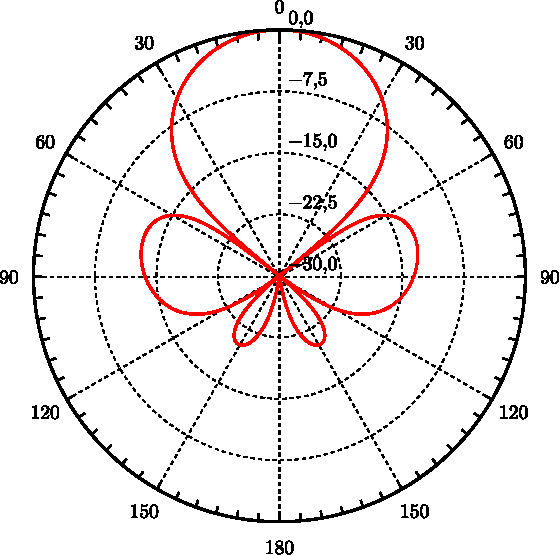
\includegraphics[scale = 1]{Figures/Intro/intro_1.pdf}}
\subfigure[Representación cartesiana del diagrama de radiación.]{
\label{fig_intro:2}
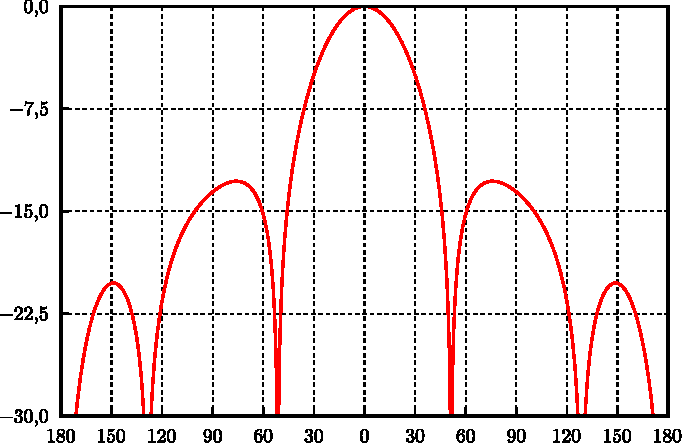
\includegraphics[scale = 1]{Figures/Intro/intro_2.pdf}}
\caption{Diagramas de radiación (dB).}
\label{grup_fig_intro:1}
\end{figure}
%%%%
Puede observarse en los diagramas de radiación una serie de lóbulos, donde es posible diferenciar los \emph{lóbulos principales}, en las direcciones de máxima radiación, y los \emph{lóbulos secundarios} o \emph{laterales}. Los lóbulos principales se definen por:
%%%%
\begin{itemize}
\item Amplitud.
\item Ancho de haz de potencia media (HPBW, \emph{Half-Power Beamwidth}): Ángulo en el que la densidad de potencia del lóbulo cae a la mitad de su valor máximo.
\item Ancho de haz entre ceros (FNBW, \emph{First-Null Beamwidth}): Separación angular entre los ceros del lóbulo.
\end{itemize}
%%%%
En el diagrama de radiación de la figura \ref{fig_intro:3} se señalan los anchos de haz de potencia media y entre ceros.
%%%%
\begin{figure} [H]
\centering 
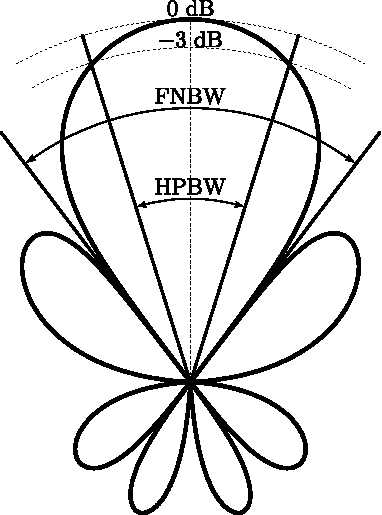
\includegraphics[scale = 1]{Figures/Intro/intro_3.pdf}
\caption{Anchos de haz de potencia media y entre ceros.}
\label{fig_intro:3}
\end{figure}
%%%%

%%%%
\subsection{Directividad}
\label{subsec_intro_direc}
%%%%

%%%%
La \emph{directividad} se define como la relación entre la intensidad de radiación en una determinada dirección que produce un elemento radiante en el espacio y la intensidad de radiación promedio, o sea, la intensidad de radiación producida por un foco isotrópico alimentado con la misma potencia.
%%%%
\begin{align}
D = \frac{U}{U_0}
\label{ec_intro:9}
\end{align}
%%%%
Un radiador isotrópico es una fuente ideal cuya potencia radiada es uniforme en todas las direcciones. Si bien no existe en la práctica, proporciona una referencia isotrópica con la cual se compararán otras antenas. Debido a su radiación simétrica, el vector de Poynting no será función de los ángulos $\uptheta$ y $\upphi$, y tendrá solamente una componente radial. Su potencia total radiada está dada por:
%%%%
\begin{align}
P_{rad} = \oiint\limits_{S}\mathbf{W}_0\prodesc d\mathbf{s} = \!\int_0^{\,2\pi}\!\int_0^{\,\pi}\!W_0r^2\sen\theta\,d\theta\,d\phi = 4\pi r^2W_0
\label{ec_intro:10}
\end{align}
%%%%
y la densidad de potencia por:
%%%%
\begin{align}
W_0 = \frac{P_{rad}}{4\pi r^2}
\label{ec_intro:11}
\end{align}
%%%%
A partir de la expresión \eqref{ec_intro:11}, se determina la intensidad de radiación del radiador isotrópico.
%%%%
\begin{align}
U_0 = W_0r^2 = \frac{P_{rad}}{4\pi}
\label{ec_intro:12}
\end{align}
%%%%
La directividad, entonces, queda definida como:
%%%%
\begin{align}
D = 4\pi\frac{U}{P_{rad}}
\label{ec_intro:13}
\end{align}
%%%%
Si no se especifica la dirección, queda implícito que la dirección es la de máxima intensidad de radiación, quedando la directividad máxima expresada como:
%%%%
\begin{align}
D_0 = D_{max} = 4\pi\frac{U_{max}}{P_{rad}}
\label{ec_intro:14}
\end{align}
%%%%
Si la antena no es isotrópica, no radiará uniformemente en todas las direcciones y, por lo tanto, la intensidad de radiación dependerá de los ángulos $\uptheta$ y $\upphi$; entonces, puede expresarse la intensidad de radiación como:
%%%%
\begin{align}
&U = B_0F\left(\theta,\phi\right) \simeq \frac{r^2}{2\eta}\left[\lvert E_{\theta}\left(\theta,\phi\right)\rvert^2 + \lvert E_{\phi}\left(\theta,\phi\right)\rvert^2\right]
\label{ec_intro:15}
\end{align}
%%%%
donde $B_0$ es una constante, $E_{\theta}$ y $E_{\phi}$  son las componentes del campo eléctrico de la antena para campo lejano y $F\left(\theta,\phi\right)$ es la función que describe la variación angular de la intensidad de radiación en el espacio, denominada \emph{factor de diagrama de potencia}. El máximo valor de la expresión \eqref{ec_intro:15} está dado por:
%%%%
\begin{align}
\left.U_{max} = B_0F\left(\theta,\phi\right)\right|_{max} = B_0F_{max}\left(\theta,\phi\right)
\label{ec_intro:16}
\end{align}
%%%%
Empleando las expresiones \eqref{ec_intro:8} y \eqref{ec_intro:15}, la potencia radiada resulta:
%%%%
\begin{align}
P_{rad} = \oiint\limits_{\Omega}Ud\Omega = B_0\!\int_0^{\,2\pi}\!\int_0^{\,\pi}\!F\left(\theta,\phi\right)\sen\theta\,d\theta\,d\phi
\label{ec_intro:17}
\end{align}
%%%%
Se pueden formular las expresiones generales de la directividad y de la directividad máxima utilizando las expresiones \eqref{ec_intro:13} - \eqref{ec_intro:17}, obteniendo:
%%%%
\begin{align}
D &= 4\pi\dfrac{F\left(\theta,\phi\right)}{\displaystyle\int_0^{\,2\pi}\!\int_0^{\,\pi}\!F\left(\theta,\phi\right)\sen\theta\,d\theta\,d\phi}
\label{ec_intro:18}\\
D_0 &= 4\pi\dfrac{F_{max}\left(\theta,\phi\right)}{\displaystyle\int_0^{\,2\pi}\!\int_0^{\,\pi}\!F\left(\theta,\phi\right)\sen\theta\,d\theta\,d\phi}
\label{ec_intro:19}
\end{align}
%%%%
Relacionando las expresiones \eqref{ec_intro:18} y \eqref{ec_intro:19}, se obtiene la relación:
%%%%
\begin{align}
D &= D_0\dfrac{F\left(\theta,\phi\right)}{F_{max}\left(\theta,\phi\right)} = D_0F_n\left(\theta,\phi\right) = D_0U_n\left(\theta,\phi\right)
\label{ec_intro:20}
\end{align}
%%%%
donde $F_n\left(\theta,\phi\right)$ es el \emph{factor de diagrama de potencia normalizado}, que es coincidente con la \emph{intensidad de radiación normalizada} $U_n\left(\theta,\phi\right)$.

A partir de la expresión \eqref{ec_intro:19}, $D_0$ puede expresarse como:
%%%%
\begin{align}
D_0 = \dfrac{4\pi}{\left[\displaystyle\int_0^{\,2\pi}\!\int_0^{\,\pi}\!F\left(\theta,\phi\right)\sen\theta\,d\theta\,d\phi\right]\bigg{/}F_{max}\left(\theta,\phi\right)} = \frac{4\pi}{\Omega_A}
\label{ec_intro:21}
\end{align}
%%%%
donde $\Omega_A$ es el \emph{ángulo sólido del haz}, que se define como el ángulo sólido a través del cual fluiría toda la potencia radiada si la intensidad de radiación fuera constante e igual a la máxima dentro de dicho ángulo.

$\Omega_A$ se expresa como:
%%%%
\begin{gather}
\Omega_A = \frac{1}{F_{max}\left(\theta,\phi\right)}\int_0^{\,2\pi}\!\int_0^{\,\pi}\!F\left(\theta,\phi\right)\sen\theta\,d\theta\,d\phi = \!\int_0^{\,2\pi}\!\int_0^{\,\pi}\!F_n\left(\theta,\phi\right)\sen\theta\,d\theta\,d\phi
\label{ec_intro:22}
\end{gather}
%%%%
La expresión \eqref{ec_intro:18} describe la directividad en su forma genérica; sin embargo, muchas veces es útil emplear aproximaciones más simples, sobre todo cuando se quiere tener una idea del valor de la directividad en la dirección de máxima radiación. Para antenas muy directivas, o sea, con un único lóbulo principal y lóbulos laterales despreciables, el ángulo sólido del haz es aproximadamente igual al producto de los anchos de haz de potencia media de los dos planos perpendiculares mostrados en la figura \ref{fig_intro:4}.
%%%%
\begin{figure} [H]
\centering 
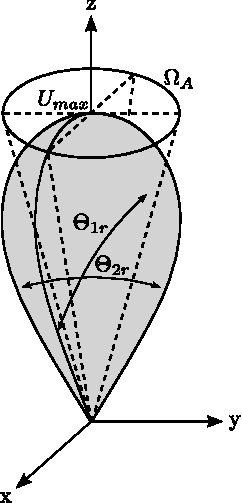
\includegraphics[scale = 1]{Figures/Intro/intro_4.pdf}
\caption{Ángulo sólido del haz.}
\label{fig_intro:4}
\end{figure}
%%%%
Con dicha aproximación, la expresión \eqref{ec_intro:21} se reduce a:
%%%%
\begin{align}
D_0 = \frac{4\pi}{\Omega_A} \simeq \frac{4\pi}{\Theta_{1r}\Theta_{2r}}
\label{ec_intro:23}
\end{align}
%%%%
El ángulo sólido del haz $\Omega_A$ se aproxima como:
%%%%
\begin{align}
\Omega_A \simeq \Theta_{1r}\Theta_{2r}
\tag{\ref{ec_intro:23}a}
\label{ec_intro:24}
\end{align}
%%%%
donde:
%%%%
\begin{align*}
\Theta_{1r} &= \text{Ancho de haz de potencia media en un plano (rad).}\\
\Theta_{2r} &= \text{Ancho de haz de potencia media en un plano en ángulo recto al otro (rad).}
\end{align*}
%%%%

%%%%
\subsection{Eficiencia}
\label{subsec_intro_eficien}
%%%%

%%%%
La \emph{eficiencia} es un parámetro utilizado para considerar las pérdidas producidas tanto en el terminal de entrada como en la estructura de la antena.

En términos generales, la eficiencia puede expresarse como:
%%%%
\begin{align}
e_0 = e_re_ce_d
\label{ec_intro:25}
\end{align}
%%%%
donde:
%%%%
\begin{align*}
e_0 = &\text{ Eficiencia total.}\\
e_g = &\,1 - \left|\Gamma\right|^2 = \text{Eficiencia por reflexiones, debida a la desadaptación de impedancias en}\\
&\text{ el terminal de entrada de la antena.}\\
e_c = &\text{ Eficiencia conductiva, debida a las pérdidas por efecto Joule.}\\
e_d = &\text{ Eficiencia dieléctrica, debida a las pérdidas dieléctricas.}
\end{align*}
%%%%
Usualmente, la eficiencia se determina considerando condiciones de adaptación ideales, por lo que $e_0$ suele expresarse como:
%%%%
\begin{align}
e_0 = e_r
\label{ec_intro:26}
\end{align}
%%%%
donde $e_r$ es la \emph{eficiencia de radiación de la antena}.
%%%%

%%%%
\subsection{Ganancia}
\label{subsec_intro_ganancia}
%%%%

%%%%
Se define como \emph{ganancia} a la relación entre la intensidad de radiación en una determinada dirección que produce un elemento radiante en el espacio y la intensidad de radiación que se obtendría si la potencia de entrada de la antena se irradiara isotrópicamente. La intensidad de radiación correspondiente a la potencia radiada isotrópicamente es igual a la potencia de entrada de la antena dividida por $4\pi$, por lo que la ganancia puede expresarse como:
%%%%
\begin{align}
G = 4\pi\frac{U}{P_{in}}
\label{ec_intro:27}
\end{align}
%%%%
Debido a las pérdidas existentes en la antena, la potencia radiada no será la misma que la potencia de entrada; es posible entonces relacionar ambas potencias mediante la eficiencia de radiación.
%%%%
\begin{align}
P_{rad} = e_rP_{in}
\label{ec_intro:28}
\end{align}
%%%%
La ganancia puede expresarse como:
%%%%
\begin{align}
G = e_r4\pi\frac{U}{P_{rad}}
\label{ec_intro:29}
\end{align}
%%%%
por lo que es posible relacionar la ganancia con la directividad.
%%%%
%%
\begin{align}
G = e_rD
\label{ec_intro:30}
\end{align}
%%
%%%%

%%%%
\subsection{Eficiencia del haz}
\label{subsec_intro_efi_haz}
%%%%

%%%%
La \emph{eficiencia del haz} $\varepsilon_M$ es un indicador del porcentaje de la potencia total radiada por la antena que se concentra en el haz principal. El ángulo sólido del haz está conformado por las contribuciones del lóbulo principal y de los lóbulos secundarios, por lo que:
%%%%
\begin{align}
\Omega_A = \Omega_M + \Omega_m
\label{ec_intro:31}
\end{align}
%%%%
donde:
%%%%
\begin{align*}
\Omega_M &= \text{Ángulo sólido del haz principal (sr).}\\
\Omega_m &= \text{Ángulo sólido de los haces laterales (sr).}
\end{align*}
%%%%
La eficiencia del haz, entonces, se define como:
%%%%
\begin{align}
\varepsilon_M = \frac{\Omega_M}{\Omega_A}
\label{ec_intro:32}
\end{align}
%%%%

%%%%
\subsection{Impedancia de entrada}
\label{subsec_intro_imp_ent}
%%%%

%%%%
La \emph{impedancia de entrada} se define como la impedancia que presenta la antena en sus terminales de entrada al circuito de alimentación. Generalmente es compleja, y puede expresarse como:
%%%%
\begin{align}
Z_A = R_A + jX_A
\label{ec_intro:33}
\end{align}
%%%%
donde:
%%%%
\begin{align*}
Z_A &= \text{Impedancia de entrada ($\Omega$).}\\
R_A &= \text{Resistencia de entrada ($\Omega$).}\\
X_A &= \text{Reactancia de entrada ($\Omega$).}
\end{align*}
%%%%
La parte resistiva de la impedancia de entrada está compuesta por dos componentes:
%%%%
\begin{align}
R_A = R_R +R_L
\label{ec_intro:34}
\end{align}
%%%%
donde:
%%%%
\begin{align*}
R_R &= \text{Resistencia de radiación de la antena ($\Omega$).}\\
R_L &= \text{Resistencia de pérdidas de la antena ($\Omega$).}
\end{align*}
%%%%
Si se asume que la antena es excitada con un generador con impedancia interna:
%%%%
\begin{align}
Z_G = R_G + jX_G
\label{ec_intro:35}
\end{align}
%%%%
donde:
%%%%
\begin{align*}
R_G &= \text{Resistencia de la impedancia del generador ($\Omega$).}\\
X_G &= \text{Reactancia de la impedancia del generador ($\Omega$).}
\end{align*}
%%%%
y la antena es usada como transmisora, puede representarse la antena y el generador por el circuito equivalente Thevenin de la figura \ref{fig_intro:5}.
%%%%
\begin{figure} [H]
\centering 
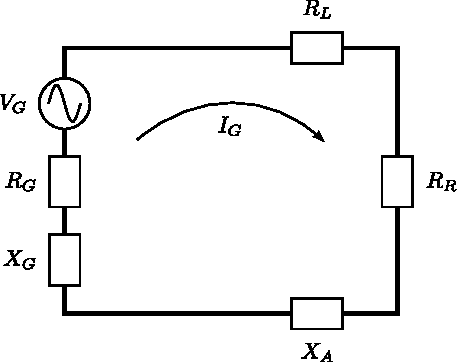
\includegraphics[scale = 1]{Figures/Intro/intro_5.pdf}
\caption{Circuito equivalente Thevenin de la antena en modo transmisora.}
\label{fig_intro:5}
\end{figure}
%%%%
Para determinar la potencia radiada (entregada a $R_R$) y la potencia disipada por efecto Joule (entragada a $R_L$), primero se determina la corriente que circula por el circuito equivalente, que  está dada por:
%%%%
\begin{align}
I_G = \frac{V_G}{Z_A + Z_G} = \frac{V_G}{\left(R_R + R_L + R_G\right) + j\left(X_A + X_G\right)}
\label{ec_intro:36}
\end{align}
%%%%
La potencia radiada por la antena está dada por:
%%%%
\begin{align}
P_R = \frac{1}{2}\left|I_G\right|^2R_R = \frac{\left|V_G\right|^2}{2}\left[\frac{R_R}{\left(R_R + R_L + R_G\right)^2 + \left(X_A + X_G\right)^2}\right]
\label{ec_intro:37}
\end{align}
%%%%
y la potencia disipada por efecto Joule por:
%%%%
\begin{align}
P_L = \frac{1}{2}\left|I_G\right|^2R_R = \frac{\left|V_G\right|^2}{2}\left[\frac{R_L}{\left(R_R + R_L + R_G\right)^2 + \left(X_A + X_G\right)^2}\right]
\label{ec_intro:38}
\end{align}
%%%%
La potencia restante se disipa sobre la resistencia interna del generador $R_G$, cuya expresión es:
%%%%
\begin{align}
P_G = \frac{1}{2}\left|I_G\right|^2R_R = \frac{\left|V_G\right|^2}{2}\left[\frac{R_G}{\left(R_R + R_L + R_G\right)^2 + \left(X_A + X_G\right)^2}\right]
\label{ec_intro:39}
\end{align}
%%%%
La máxima transferencia de potencia a la antena se produce cuando la impedancia de entrada de la antena es la conjugada de la impedancia interna del generador, o sea:
%%%%
\begin{gather}
R_R + R_L = R_G
\label{ec_intro:40}\\
X_A = - X_G
\label{ec_intro:41}
\end{gather}
%%%%
En este caso, las potencias involucradas son:
%%%%
\begin{align}
P_R &= \frac{\left|V_G\right|^2}{8}\left[\frac{R_R}{\left(R_R + R_L\right)^2}\right]
\label{ec_intro:42}\\
P_L &= \frac{\left|V_G\right|^2}{8}\left[\frac{R_L}{\left(R_R + R_L\right)^2}\right]
\label{ec_intro:43}\\
P_G &= \frac{\left|V_G\right|^2}{8}\left[\frac{1}{R_R + R_L}\right]
\label{ec_intro:44}
\end{align}
%%%%
Puede observarse que $P_G = P_R + P_L$, por lo que de la potencia provista por el generador, la mitad se disipa en la resistencia interna $R_G$ y la otra mitad es entregada a la antena, de la cual parte se disipa por efecto Joule y parte se irradia. Esta condición, la de máxima transferencia de potencia, se cumple cuando existe \emph{adaptación de impedancias}. Si la antena idealmente no tuviera pérdidas, el generador debería suministrar el doble de la potencia que se desea irradiar en la condición de máxima transferencia de potencia. En la práctica la potencia suministrada por el generador debe ser mayor, para compensar las pérdidas óhmicas tanto en la antena como en las líneas de transmisión. Una medida de las pérdidas en la antena surge a partir de la \emph{eficiencia de radiación}, que puede expresarse como:
%%%%
\begin{align}
e_r = \frac{R_R}{R_R + R_L}
\label{ec_intro:45}
\end{align}
%%%%

%%%%
\subsection{Area efectiva}
\label{subsec_intro_area_efec}
%%%%

%%%%
Cuando una antena se utiliza como receptora, recibe una determinada densidad de potencia de la onda incidente que convierte en potencia eléctrica. Se define como \emph{área efectiva} a la relación entre la potencia que la onda proporciona a una carga conectada a la antena receptora y la densidad de potencia de la onda incidente. El área efectiva puede expresarse como:
%%%%
\begin{align}
A_e = \frac{P_T}{W_i}
\label{ec_intro:46}
\end{align}
%%%%
donde:
%%%%
\begin{align*}
A_e &= \text{Área efectiva (m$^2$).}\\
P_T &= \text{Potencia proporcionada a la carga (W).}\\
W_i &= \text{Densidad de potencia de la onda incidente (W/m$^2$).}
\end{align*}
%%%%
Con el fin de entender claramente el concepto de área efectiva, en la figura \ref{fig_intro:6} se muestra el circuito equivalente Thevenin de una antena receptora conectada a una carga $Z_T$.
%%%%
\begin{figure} [H]
\centering 
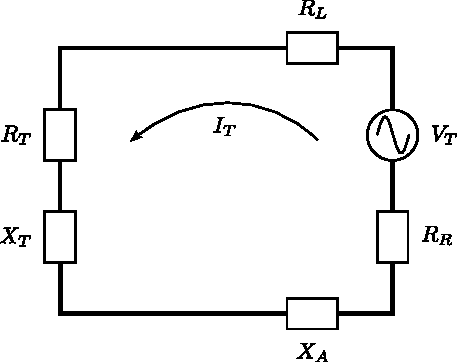
\includegraphics[scale = 1]{Figures/Intro/intro_6.pdf}
\caption{Circuito equivalente Thevenin de la antena en modo receptora.}
\label{fig_intro:6}
\end{figure}
%%%%
donde:
%%%%
\begin{align}
Z_T = R_T + jX_T
\label{ec_intro:47}
\end{align}
%%%%
La potencia proporcionada a la resistencia $R_T$ está dada por:
%%%%
\begin{align}
P_T = \frac{\left|V_T\right|^2}{2}\left[\frac{R_T}{\left(R_R + R_L + R_T\right)^2 + \left(X_A + X_T\right)^2}\right]
\label{ec_intro:48}
\end{align}
%%%%
y la potencia disipada por efecto Joule por:
%%%%
\begin{align}
P_L = \frac{\left|V_T\right|^2}{2}\left[\frac{R_L}{\left(R_R + R_L + R_T\right)^2 + \left(X_A + X_T\right)^2}\right]
\label{ec_intro:49}
\end{align}
%%%%
La potencia restante se dispersa al espacio, o sea, se disipa sobre la resistencia de radiación $R_R$, y su expresión es:
%%%%
\begin{align}
P_R = \frac{\left|V_T\right|^2}{2}\left[\frac{R_R}{\left(R_R + R_L + R_T\right)^2 + \left(X_A + X_T\right)^2}\right]
\label{ec_intro:50}
\end{align}
%%%%
En condiciones de adaptación, las potencias quedan expresadas como:
%%%%
\begin{align}
P_T &= \frac{\left|V_T\right|^2}{8R_T}
\label{ec_intro:51}\\
P_L &= \frac{\left|V_T\right|^2}{8}\left[\frac{R_L}{\left(R_R + R_L\right)^2}\right]
\label{ec_intro:52}\\
P_R &= \frac{\left|V_T\right|^2}{8}\left[\frac{R_R}{\left(R_R + R_L\right)^2}\right]
\label{ec_intro:53}
\end{align}
%%%%
y puede observarse que $P_T = P_R + P_L$. Para este caso, y si la antena está orientada para recibir máxima señal (es decir, orientada hacia donde la directividad es igual a la directividad máxima $D_0$), el área efectiva se denomina \emph{área efectiva máxima}. El área efectiva máxima está relacionada con el área física de la antena mediante la \emph{eficiencia de abertura}, cuya expresión es:
%%%%
\begin{align}
\varepsilon_{ap} = \frac{A_{em}}{A_p}
\label{ec_intro:54}
\end{align}
%%%%
donde:
%%%%
\begin{align*}
\varepsilon_{ap} &= \text{Eficiencia de abertura.}\\
A_{em} &= \text{Área efectiva máxima (m$^2$).}\\
A_p &= \text{Área física (m$^2$).}
\end{align*}
%%%%
Se cumplirá siempre que $0 \leq\varepsilon_{ap}\leq 1$. Si se asumen pérdidas por efecto Joule nulas ($R_L = 0$), la potencia entregada a la carga será igual a la potencia que la antena dispersa en el espacio, o sea, habrá una potencia reirradiada exactamente igual a la recibida.

Para determinar la relación entre el área efectiva máxima y la directividad, se parte de un enlace entre dos antenas, físicamene ubicadas en el espacio libre y separadas por una distancia $R$, como se muestra en la figura \ref{fig_intro:7}.
%%%%
\begin{figure} [H]
\centering 
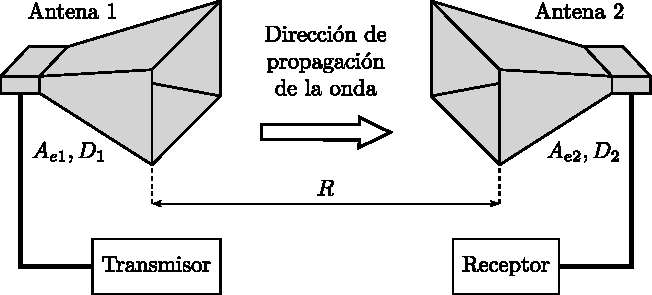
\includegraphics[scale = 1]{Figures/Intro/intro_7.pdf}
\caption{2 antenas separadas por una distancia $R$.}
\label{fig_intro:7}
\end{figure}
%%%%
En primera instancia, se asume que la antena 1 es la transmisora y la antena 2 es la receptora. La densidad de potencia radiada por la antena 1 a una distancia $R$ responde a la expresión:
%%%%
\begin{align}
W_1 = \frac{P_TD_1}{4\pi R^2}
\label{ec_intro:55}
\end{align}
%%%%
La potencia recibida por la antena 2 es:
%%%%
\begin{align}
P_2 = A_{e2}W_1 = A_{e2}\frac{P_TD_1}{4\pi R^2}
\label{ec_intro:56}
\end{align}
%%%%
por lo que:
%%%%
\begin{align}
D_1A_{e2} = \frac{P_2}{P_T}\,4\pi R^2
\tag{\ref{ec_intro:56}a}
\label{ec_intro:57}
\end{align}
%%%%
Si ahora la antena 2 es usada como transmisora y la antena 1 como receptora, puede expresarse que:
%%%%
\begin{align}
D_2A_{e1} = \frac{P_1}{P_T}\,4\pi R^2
\label{ec_intro:58}
\end{align}
%%%%
por lo que a partir de las expresiones \eqref{ec_intro:57} y \eqref{ec_intro:58} se llega a:
%%%%
\begin{align}
\frac{D_1}{A_{e1}} = \frac{D_2}{A_{e2}}
\label{ec_intro:59}
\end{align}
%%%%
El incremento de la directividad genera un aumento del área efectiva, por lo que:
%%%%
\begin{align}
\frac{D_{01}}{A_{em1}} = \frac{D_{02}}{A_{em2}}
\label{ec_intro:60}
\end{align}
%%%%
Suponiendo que la antena 1 es un foco isotrópico, su directividad sería unitaria, por lo que:
%%%%
\begin{align}
A_{em1} = \frac{A_{em2}}{D_{02}}
\label{ec_intro:61}
\end{align}
%%%%
Considerando ahora que la antena 2 es un dipolo de Hertz, su área efectiva máxima, asumiendo que las pérdidas óhmicas son nulas, está expresada por:
%%%%
\begin{align}
A_{em} = \frac{\left|V_T\right|^2}{8W_iR_R}
\label{ec_intro:62}
\end{align}
%%%%
Como el dipolo es muy corto, puede asumirse que el campo inducido es constante y de fase uniforme, por lo que la tensión inducida es:
%%%%
\begin{align}
V_T = El
\label{ec_intro:63}
\end{align}
%%%%
donde:
%%%%
\begin{align*}
V_T &= \text{Tensión inducida en el dipolo (V).}\\
E &= \text{Campo eléctrico de la onda incidente (V/m).}\\
l &= \text{Longitud del dipolo (m).}
\end{align*}
%%%%
Para una onda incidente plana, la densidad de potencia incidente puede expresarse como:
%%%%
\begin{align}
W_i = \frac{E^2}{2\eta}
\label{ec_intro:64}
\end{align}
%%%%
La resistencia de radiación del dipolo de Hertz está dada por \cite{Fano2}:
%%%%
\begin{align}
R_R = 80\left(\frac{\pi l}{\lambda}\right)^2
\label{ec_intro:65}
\end{align}
%%%%
El área efectiva máxima, entonces, puede expresarse como:
%%%%
\begin{align}
A_{em} = \frac{\left(El\right)^2}{8\,\dfrac{E^2}{2\eta}\,80\left(\dfrac{\pi l}{\lambda}\right)^2} = \frac{3\lambda^2}{8\pi}
\label{ec_intro:66}
\end{align}
%%%%
Para un dipolo de Hertz, la directividad máxima es \cite{Fano2}:
%%%%
\begin{align}
D_0 = \frac{3}{2}
\label{ec_intro:67}
\end{align}
%%%%
Puede entonces determinarse el área efectiva máxima de un foco isotrópico, cuya expresión final es:
%%%%
\begin{align}
A_{em} = \frac{\lambda^2}{4\pi}
\label{ec_intro:68}
\end{align}
%%%%
En forma general, entonces, puede expresarse el área efectiva máxima en función de la directividad máxima $D_0$ mediante la expresión:
%%%%
\begin{align}
A_{em} = \frac{\lambda^2}{4\pi}D_0
\label{ec_intro:69}
\end{align}
%%%%
Si existen pérdidas óhmicas y dieléctricas en la antena, su área efectiva máxima debe modificarse para tener en cuenta tales pérdidas, por lo que:
%%%%
\begin{align}
A_{em} = e_r\frac{\lambda^2}{4\pi}D_0 = \frac{\lambda^2}{4\pi}G_0
\label{ec_intro:70}
\end{align}
%%%%

%%%%
\subsection{Polarización}
\label{subsec_intro_polar}
%%%%

Se define como \emph{polarización de una onda electromagnética} a la dirección del vector intensidad del campo eléctrico $\mathbf{E}$, o sea, la dirección en la cual el campo eléctrico varía temporalmente.

El campo eléctrico $\mathbf{E}$ puede expresarse como la suma de dos componentes ortogonales $E_x$ y $E_y$, con una diferencia de fase temporal $\delta$ entre las mismas, es decir:
%%%%
\begin{align}
\mathbf{E} = E_x\,\versor{x} + E_y\,\versor{y} =  E_{0x}\cos\left(\omega t\right)\versor{x} + E_{0y}\cos\left(\omega t + \delta\right)\versor{y}
\label{ec_intro:71}
\end{align}
%%%%
donde:
%%%%
\begin{align*}
E_{0x} &= \text{Amplitud de la componente }E_x\text{ (V/m).}\\
E_{0y} &= \text{Amplitud de la componente }E_y\text{ (V/m).}
\end{align*}
%%%%
Ambas componentes son perpendiculares a la dirección de propagación, que coincide con la dirección del eje \emph{z}.

Las polarizaciones más comúnmente empleadas en la práctica son:
%%%%
\begin{enumerate}
\item Polarización lineal vertical: El campo eléctrico varía temporalmente sobre el eje \emph{y} al propagarse, por lo que la expresión resultante del campo eléctrico $\mathbf{E}$ es:
%%%%
\begin{align}
\mathbf{E} = E_y\,\versor{y} =  E_{0y}\cos\left(\omega t\right)\versor{y}
\label{ec_intro:72}
\end{align}
%%%%
\item Polarización lineal horizontal: El campo eléctrico varía temporalmente sobre el eje \emph{x} al propagarse, por lo que la expresión resultante del campo eléctrico $\mathbf{E}$ es:
%%%%
\begin{align}
\mathbf{E} = E_x\,\versor{x} =  E_{0x}\cos\left(\omega t\right)\versor{x}
\label{ec_intro:73}
\end{align}
%%%%
\item Polarización circular: El campo eléctrico varía temporalmente describiendo una circunsferencia al propagarse, por lo que la expresión resultante del campo eléctrico $\mathbf{E}$ es:
%%%%
\begin{align}
\mathbf{E} = E_x\,\versor{x} + E_y\,\versor{y} =  E_{0}\cos\left(\omega t\right)\versor{x} \pm E_{0}\sen\left(\omega t\right)\versor{y}
\label{ec_intro:74}
\end{align}
%%%%
Para que la polarización sea circular, debe cumplirse que:
%%%%
\begin{align}
E_{0x} &= E_{0y} = E_0
\label{ec_intro:75}\\
\delta &= \pm\left(2n + 1\right)\dfrac{\pi}{2}
\label{ec_intro:76}
\end{align}
%%%%
\end{enumerate}
%%%%
En la práctica, las antenas se diseñan para que trabajen con una determinada polarización; cualquier componente existente con otra polarización no es deseada y debe ser lo menor posible. A tal efecto, se define:
%%%%
\begin{itemize}
\item Copolarización: Es la componente del campo eléctrico $\mathbf{E}$ con la polarización deseada.
\item Polarización cruzada: Es la componente del campo eléctrico $\mathbf{E}$ cuya polarización no es la deseada y que es ortogonal a la copolarización.
\end{itemize}
%%%%
Si la antena es diseñada para que trabaje con polarización lineal vertical, es decir, que la copolarización se corresponda con la polarización en el eje \emph{y}, la polarización cruzada corresponderá a las componentes del campo eléctrico $\mathbf{E}$ con polarización en el eje \emph{x}.

Para determinar la relación entre las amplitudes de las componentes ortogonales de polarización lineal, se define la \emph{relación de polarización lineal} $\rho_L$ \cite{Fano2}, o simplemente \emph{relación de polarización cruzada}, cuya expresión es:
%%%%
\begin{align}
\rho_L &= \dfrac{E_{0y}}{E_{0x}}
\label{ec_intro:77}
\end{align}
%%%%
En dB, la expresión \eqref{ec_intro:77} resulta:
%%%%
\begin{align}
\rho_L &= 20\log\left(E_{0y}\right) -  20\log\left(E_{0x}\right)
\label{ec_intro:78}
\end{align}
%%%%

\chapter{Fundamentos de estructuras de banda prohibida electromagnética (EBG)}
\label{cap_fundamentos}
\lhead{Capítulo \ref{cap_fundamentos}. \emph{Fundamentos de EBG}} 
%%%%%%%%%%%%%%%%%%%%%%%%%%
%%  Capítulo 2: Fundamentos de estructuras de banda prohibida electromagnética (EBG)}  %%
%%%%%%%%%%%%%%%%%%%%%%%%%%

%%%%
\section{Reseña histórica: Metamateriales, materiales periódicos y EBGs}
\label{sec_resenia_metamateriales}
%%%%
% EBGs in Antennas, Rahmat (libro). Pagina 2.
% Explicación de los métodos de análisis
% Uso para low profile antennas
% Engheta, pag 215
% Caloz, ^pag 17
% Caloz Pag 20
% Caloz pag 83, diferencia con filtros
% Pozar, pag 380
% Pozar, p 424. Stepped impedance filters.
% Pozar, bandstop filter design, pag 440
% Tabla interesante: Baccarello, Paulotto, impreso.
% stack de capas o cristal? Brown, McMahon, Parker. Ademas linda foto.
% Relación con soft-hard surfaces. Gao, chen, wang, yang-
% Discusión terminológica: Oliner.
% ITOH, Pediodic structures.
% DGS, tesis de ABIDIN, pag2. Tiene intro histórica.
% ABIDIN, tesis, pagina 16: Def de EBG. imagen interesante.
% Venkateswaran, algunos ejemplos de EBGs.
% Importancia de EBGs. Venkateswaran tesis, pag 1.
% Algo de intro: Pagina 4, tesis Zheng.

Los EBG (Materiales de banda prohibida electromagnética, \textit{Electromagnetic Bandgap Materials}), PBG (Materiales de banda prohibida fotónica, \textit{Photonic Bandgap Materials}) o cristales fotónicos son un tipo de estructura artificial, dieléctrica o metalodieléctrica, con capacidades para controlar ondas electromagnéticas \cite{Engheta} a partir de una variación periódica en el espacio de la constante dieléctrica, permitiendo que las mismas se propaguen sólo en direcciones determinadas, o impedir su propagación completamente. Esta capacidad proviene de su estructura de banda prohibida electromagnética, que surge en analogía al concepto de banda prohibida electrónica, que controla el movimiento de ondas de electrones que viajan en un potencial periódico cristalino.

En 1946, Louis Brillouin publicó su libro sobre ondas mecánicas, "\textit{Wave propagation in periodic structures: Electric filters and crystal lattices}" \cite{Brillouin:WavePropagation}, donde demostró que un arreglo periódico impone restricciones a los vectores de onda $k$ que pueden propagarse por él, dado que da lugar a condiciones de contorno para los modos permitidos. Aquellas ondas que no cumplieran las condiciones de borde impuestas, no podrían propagarse. La propagación de ondas sobre superficies periódicas había comenzado a estudiarse, para ondas electromagnéticas, con anterioridad al trabajo de Brillouin, aunque a partir del mismo se formalizó el desarrollo de las aplicaciones para microondas.

En 1968, el físico ruso Viktor Veselago describió por primera vez, de forma teórica, la posibilidad de que existieran materiales con índice de refracción negativo, denominados LHS (\textit{Left Handed Materials}, materiales de mano izquierda), con permitividad eléctrica y permeabilidad magnética negativas, de modo que la velocidad de fase de una onda que se propagara por ese medio fuera antiparalela a la velocidad de grupo. Treinta años más tarde, Pendry propuso la primera forma de fabricación de un medio con esas características en una banda limitada de frecuencia, utilizando SSRs (Split-ring resonators, resonadores de aro dividido), responsables de la permeabilidad magnética negativa, y cables conductores, responsables de la permitividad eléctrica negativa. Recién en el año 2000 se construyó el primer metamaterial sobre las propuestas de Pendry, y varios experimentos confirmaron refracción negativa en los mismos.

La primera descripción de estructuras dieléctricas periódicas con una banda prohibida completa fue dada, en 1990, por Ho, Chan y Soukoulis, en Iowa, Estados Unidos, quienes propusieron un arreglo periódico de esferas dieléctricas, dispuestas en forma de capas. Para un rango amplio de radios de esferas, el efecto de banda prohibida se daba en todas direcciones. Hacia fines de la década de 1980, Yablonovitch divisó una estructura cristalina simétrica de más fácil fabricación, que consistía en la producción de tres agujeros cilíndricos en un prisma dieléctrico, repetido periódicamente. Demostró, además, usando dichas estructuras, que la existencia de una banda prohibida electromagnética podía ser predicha teóricamente, en base, principalmente, a la constante de periodicidad del dieléctrico artificial.

Los trabajos de Yablonovitch y Pendry se hicieron sobre estructuras con banda de interés en microondas, pero bajo modelos fotónicos, gracias a la linealidad de las ecuaciones de Maxwell, lo que permitió el uso de distintas técnicas conocidas y desarrolladas durante el siglo XX en microondas para el diseño de materiales fotónicos de estas características a partir de finales de la década de 1990, aunque principalmente en ámbitos de investigación de ciencias básicas, sin un interés marcado de la industria.

Las denominadas "superficies electromagnéticas" (\textit{electromagnetic surfaces}) consisten en superficies texturadas que imponen condiciones de contorno particulares, capaces de lograr cambiar la polarización de una onda incidente, influir sobre las ondas de superficie y controlar la fase de reflexión. La más simple consiste en una placa metálica coarrugada, como la mostrada en la figura \ref{fig:superficie-coarrugada}, de forma que las variaciones de altura sean de $\lambda/4$, que puede comportarse como una "superficie blanda" (\textit{soft surface}) o una "superficie dura" (\textit{hard surface}), en función de la polarización de la onda que se propaga.

\section{Difracción de Bragg}
\label{sec_bragg}
%%%%
% Caloz, pag 19
% Kamgaing (tesis), pagina22
\lipsum
\section{Bloch-Floquet}
\label{sec_bloch}
%%%%
\lipsum
% Libro de rahmat. Pagina 46.
% Zona de brillouin. Rahmat, libro, pagina 31.
% Diagrama de dispersión. Página 67 Rahmat. Caloz: pagina 106.
% Impedancia de Bloch: Caloz, pagina 113
% Tesis Choi, pag 82.
% Tesis Kovacs, pag 13.
% Venkateswaran, pag 26.
% Tesis Zheng, pag 5-8
\section{Impedancia de onda y de superficie}
\label{sec_imp_superficie}
%%%%
% Rahmat. Pagina 77 libro.
% Engheta, pagina 290.
\lipsum


\section{Metamateriales ópticos: Cristales fotónicos}
\label{sec_cristales_fotonicos}
%%%%
\lipsum
% Lightline stuff. Rahmat, pagina 28. Caloz, pagina 139. Pozar pag 386
\section{Tipos de EBG}
\label{sec_tipos_mtm}
%%%%
\lipsum[1]
% Tesis de kovacs, pagina 7.
\subsection{EBGs de mano izquierda}
\label{subsec_ebg_izquierda}
%%%%
\lipsum
% Caloz, Pag 27, 43, 
\subsection{EBGs uniplanares}
\label{subsec_ebg_uniplanar}
%%%%
\lipsum
% buena intro en rahmat (libro), pagina 35-37
% Buscar las distintas formas, incluyendo Peano. Relación con FSS.
% Buena intro esn Goussetis, Feresidis, Vardaxoglou.
% Diseños para incidencia obliucua: Kim, Yand, Elsherbeni. Tambien en Lin, Li, Zhang.
% Hilbert: McVAy, Engheta, Hoorfar.
% Power loss analysis: Mohajer-Iravani, Ramahi, de Hindawi corp.
% Kern, Douglas, Werner.
% Analisis en Goussetis, Feresidis, paper posta. Tipos de resonancia.
% Lamminen, Vimpari, Saily. 
% Maci, Caiazzo, Cucini. Jodido, interesante. Leer.
\section{Modelado y simulación de metamateriales}
\label{sec_simulacion_mtm}
%%%%
\lipsum
% Un modelado medio simple se puede ver en la tesis de Choi, pag 90-99
\subsection{Métodos de cavidades periódicas}
\label{subsec_eigenfunctions}
%%%%
\lipsum
% Fullwave: Baccarello, Paulotto, impreso.
% Hacer estudio gráfico similar al CALOZ, pag 176.
\subsection{Modelado por líneas de transmisión}
%%%%
\lipsum
% Caloz, pag 60, 67, 76, 79
% Bidimensional, Caloz, pag 133
% Rahman Stuchly.ç
% Calculo de la inductancia de meander inductors: Stojanovic, Zivanov
% Cuentas! Wu, Lin, Wang, Wang, Chen
% Kim, Schutt-Ainé, 178. Modelado para PDN.
%Venkateswaran, pag 40 en adelante.
% Impedancia: hacer algo similar. Tesis Zheng, pag 8

\subsubsection{TMM}
%%%%
\lipsum[2]
% Caloz, pagina 144
% Choi (tesis), pag 54
\subsubsection{TLM}
\label{subsubsec_tlm}
%%%%
\lipsum
% Caloz, pag 155

\chapter{Modelado y simulación de metamateriales}
\label{cap_principios}
\lhead{Capítulo \ref{cap_principios}. \emph{Principios de reflectores parabólicos}} 
%%%%%%%%%%%%%%%%%%%%%%%%%
%%  Capítulo 3: Principios de reflectores parabólicos  %%
%%%%%%%%%%%%%%%%%%%%%%%%%

%%%%
\section{Introducción}
\label{sec_principios_intro}
%%%%

%%%%
Lo que comúnmente se conoce como antena parabólica está en realidad compuesto por dos elementos: la antena propiamente dicha, que cumple la función de iluminador o alimentador, y la superficie reflectora, que consiste en un paraboloide de revolución.
%%%%
\begin{figure}[H]
\centering
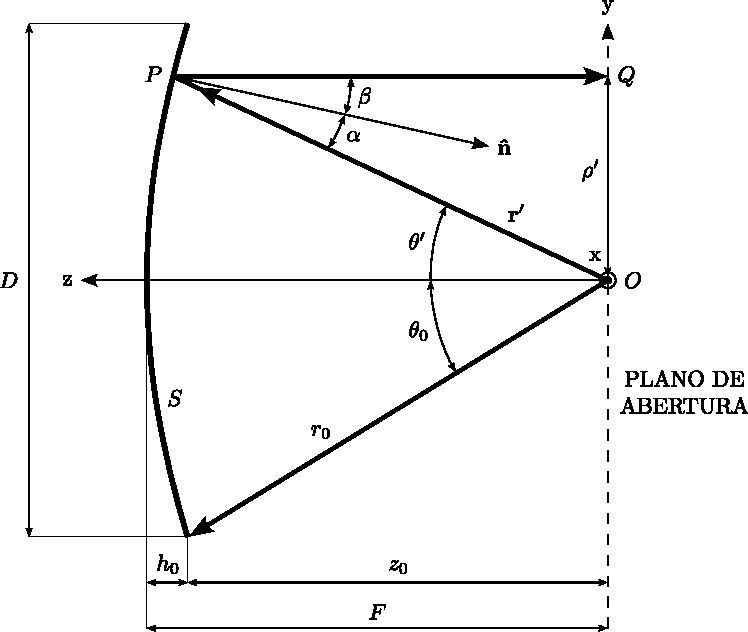
\includegraphics[scale = 0.97]{Figures/Principios/principios_1}
\caption{Esquema bidimensional de un reflector parabólico.}
\label{fig_principios:1}
\end{figure}
%%%%
En la figura \ref{fig_principios:1} puede observarse un esquema bidimensional de un reflector parabólico. La ecuación que describe la curva parabólica resultante de la intersección entre el paraboloide de revolución y cualquier plano que contenga al eje \emph{z}, en función de la distancia focal $F$, es:
%%%%
\begin{align}
{\rho '}^2 = 4F\left(F - z'\right),\hspace{5mm}\rho '\leq\frac{D}{2}
\label{ec_principios:1}
\end{align}
%%%%
Para un desplazamiento dado $\rho '$ desde el eje del reflector, $r'$ es la distancia entre el punto $P$ sobre la superficie del reflector y el punto focal $O$. La curva parabólica puede expresarse también en coordenadas polares como:
%%%%
\begin{align}
r' = \frac{2F}{1 + \cos\theta '} = F\sec^2\left(\frac{\theta '}{2}\right)
\label{ec_principios:2}
\end{align}
%%%%
y la proyección de $r'$ sobre el plano de abertura es:
%%%%
\begin{align}
\rho ' = r'\sen\theta ' = \frac{2F\sen\theta '}{1 + \cos\theta '} = 2F\tan\left(\frac{\theta '}{2}\right)
\label{ec_principios:3}
\end{align}
%%%%
Comúnmente, la curvatura del reflector se expresa en términos de $F/D$ y $\theta_0$, donde $F/D$ es la \emph{relación distancia focal-diámetro} y $\theta_0$ es el \emph{ángulo de abertura máximo}, formado entre el punto focal $O$ y el borde del reflector. A partir de la figura \ref{fig_principios:1} puede determinarse la relación entre $F/D$ y $\theta_0$, cuya expresión resulta:
%%%%
\begin{align}
\dfrac{F}{D} = \frac{1}{4}\cot\left(\frac{\theta_0}{2}\right)
\label{ec_principios:4}
\end{align}
%%%%
y su gráfica puede observarse en la figura \ref{fig_principios:2}.
%%%%
\begin{figure}[H]
\begin{minipage}{.5\textwidth}
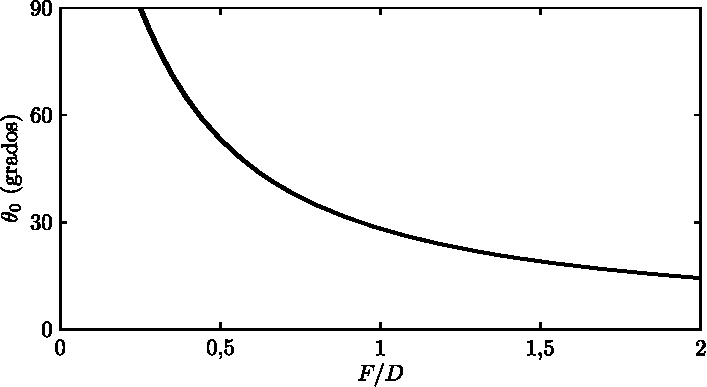
\includegraphics[scale = 1]{Figures/Principios/principios_2}
\end{minipage}
\begin{minipage}{.5\textwidth}
\hfill
\begin{tabular}{cc}
$F/D$ & $\theta_0$ \\
\hline
0,25 & 90,0$^{\circ}$\\
0,30 & 79,6$^{\circ}$\\
0,33 & 73,7$^{\circ}$\\
0,40 & 64,0$^{\circ}$\\
0,50 & 53,1$^{\circ}$\\
1,00 & 28,1$^{\circ}$\\
\\
\end{tabular}
\end{minipage}
\caption{Angulo $\theta_0$ en función de $F/D$.}
\label{fig_principios:2}
\end{figure}
%%%%
A partir de la óptica geométrica (GO) surgen las siguientes propiedades de gran importancia de los reflectores parabólicos:
\begin{enumerate}
\item Los rayos que emergen del punto focal $O$ se coliman luego de reflejarse en la superficie metálica del reflector, y los rayos reflejados son paralelos al eje del reflector (eje \emph{z}).
\item La longitud de todos los caminos que describen los rayos desde el punto focal $O$ hasta el plano de abertura, luego de reflejarse en la superficie metálica del reflector, es la misma e igual a $2F$.
\end{enumerate}
%%%%
La primera propiedad se dedude directamente de la aplicación de la ley de reflexión de Snell en la superficie del reflector, o sea, tomando que $\alpha = \beta$. Para demostrar esto, primero se determina la superficie normal al punto de reflexión $P$ evaluando el gradiente de la ecuación de la curva parabólica $S = F - r'\cos^2\left(\theta '/2\right) = 0$, basada en la expresión \eqref{ec_principios:2}; entonces:
%%%%
\begin{align}
\begin{split}
\mathbf{N} &= \nabla S = \nabla\left[f - r'\cos^2\left(\frac{\theta '}{2}\right)\right] = \left(\frac{\partial S}{\partial r'}\versor{r}' + \frac{1}{r'}\frac{\partial S}{\partial\theta '}\versor{\uptheta}'\right)\\
&= -\cos^2\left(\frac{\theta '}{2}\right)\!\versor{r}' + \cos\left(\frac{\theta '}{2}\right)\sen\left(\frac{\theta '}{2}\right)\!\versor{\uptheta}'
\end{split}
\label{ec_principios:5}
\end{align}
%%%%
Se halla la expresión del vector unitario $\versor{n}$ utilizando $|\mathbf{N}| = \cos^2\left(\dfrac{\theta '}{2}\right)$, obteniendo:
%%%%
\begin{align}
\versor{n} = \frac{\mathbf{N}}{|\mathbf{N}|} = -\cos\left(\frac{\theta '}{2}\right)\!\versor{r}' + \sen\left(\frac{\theta '}{2}\right)\!\versor{\uptheta}'
\label{ec_principios:6}
\end{align}
%%%%
Para hallar el ángulo formado entre el vector unitario $\versor{n}$, que es normal a la superficie $\mathbf{N}$ en el punto de reflexión $P$, y la onda incidente, se formula:
%%%%
\begin{align}
\cos\alpha = -\versor{r}'\prodesc\versor{n} = -\versor{r}'\prodesc\left[-\cos\left(\frac{\theta '}{2}\right)\!\versor{r}' + \sen\left(\frac{\theta '}{2}\right)\!\versor{\uptheta}'\right] = \cos\left(\frac{\theta '}{2}\right)
\label{ec_principios:7}
\end{align}
%%%%
Procediendo análogamente para hallar el ángulo formado entre el vector unitario $\versor{n}$ y la onda reflejada:
%%%%
\begin{align}
\begin{split}
\cos\beta &= -\versor{z}'\prodesc\versor{n} = -\versor{z}'\prodesc\left[-\cos\left(\frac{\theta '}{2}\right)\!\versor{r}' + \sen\left(\frac{\theta '}{2}\right)\!\versor{\uptheta}'\right]\\
&= -\left(\cos\theta '\,\versor{r}' - \sen\theta '\,\versor{\uptheta}'\right)\prodesc\left[-\cos\left(\frac{\theta '}{2}\right)\!\versor{r}' + \sen\left(\frac{\theta '}{2}\right)\!\versor{\uptheta}'\right] = \cos\left(\frac{\theta '}{2}\right)
\end{split}
\label{ec_principios:8}
\end{align}
%%%%
Comparando las expresiones \eqref{ec_principios:7} y \eqref{ec_principios:8}, puede observarse que:
%%%%
\begin{align}
\alpha = \beta = \frac{\theta '}{2}
\label{ec_principios:9}
\end{align}
%%%%
que es la expresión de la ley de reflexión de Snell. Como consecuencia de la primera propiedad, puede decirse que \emph{empleando un reflector parabólico, el frente de onda esférico radiado por una fuente ubicada en el foco emergerá a través del plano de abertura, luego de reflejarse en la superficie metálica del reflector, como un frente de onda plano}.

Para demostrar la segunda propiedad, a partir de la figura \ref{fig_principios:1} es posible expresar las distancias entre el punto focal $O$ y el punto de reflexión $P$ y entre $P$ y el punto sobre el plano de abertura $Q$ como:
%%%%
\begin{subequations}
\label{grup_ec_principios:1}
\begin{align}
\overline{OP} &= r'
\label{ec_principios:10}\\
\overline{PQ} &= r'\cos\theta
\label{ec_principios:11}
\end{align}
\end{subequations}
%%%%
y sumando ambas distancias se obtiene la longitud total del camino entre el foco y el plano de abertura luego de producirse la reflexión. Aplicando la expresión \eqref{ec_principios:2}, la longitud total queda expresada como:
%%%%
\begin{align}
\overline{OP} + \overline{PQ} = r' + r'\cos\theta ' = r'\left(1 + \cos\theta '\right) = 2F
\label{ec_principios:12}
\end{align}
%%%%
Dado que la longitud de los distintos caminos es constante e igual a $2F$, la fase de las ondas que arriben al plano de abertura desde un punto fuente ubicado en el foco también será constante. Por lo tanto, \emph{el reflector parabólico alimentado con una fuente que tenga el centro de fase en el foco generará una fase uniforme a través del plano de abertura}. Sin embargo, la distribución de amplitud en la abertura no será uniforme.

%%%%
\section{Campos radiados}
\label{sec_principios_cam_rad}
%%%%

%%%%
Para determinar las características de radiación de una antena parabólica, los dos métodos más empleados son:
\begin{itemize}
\item \emph{Método de distribución de campos sobre la abertura}: Se halla el campo reflejado sobre el plano de abertura empleando la óptica geométrica, quedando determinada una superficie circular que es la proyección del área del reflector que se denomina $S_0$, se forman las corrientes equivalentes sobre el plano de abertura, suponiendo que las fuentes son nulas fuera del área proyectada $S_0$, y luego se integran para hallar los campos radiados.
\item \emph{Método de distribución de corrientes}: Se determina la densidad de corriente inducida sobre la superficie iluminada del reflector ($S_1$ en la figura \ref{fig_principios:3}) empleando la óptica física (PO) y se hallan los campos radiados integrando la densidad de corriente inducida sobre $S_1$.
\end{itemize}
%%%%
\begin{figure}[H]
\centering
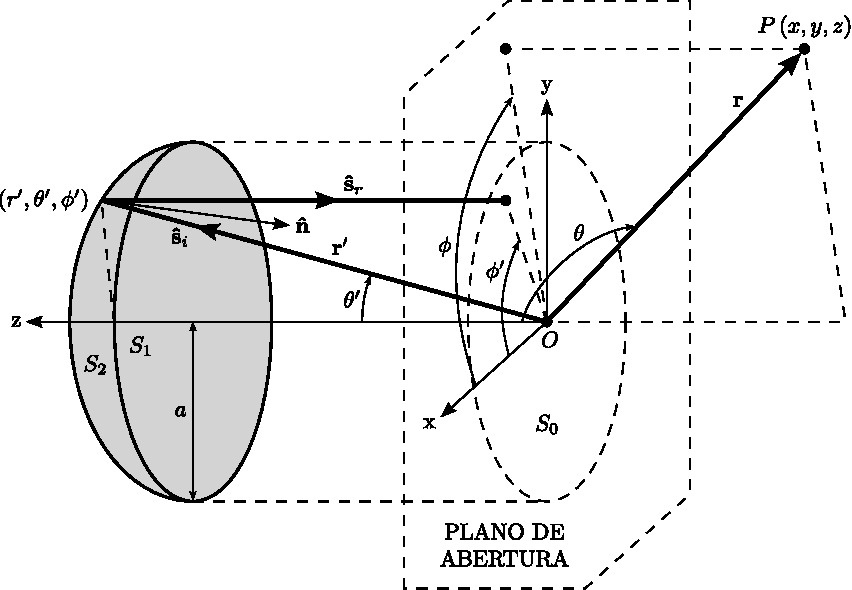
\includegraphics[scale = 1]{Figures/Principios/principios_3}
\caption{Geometría tridimensional de un reflector parabólico.}
\label{fig_principios:3}
\end{figure}
Si bien el método de distribución de campos sobre la abertura es más sencillo que el de distribución de corrientes, se emplea el segundo método debido a que se obtienen mejores aproximaciones.

Mediante la óptica física, se relaciona la densidad de corriente inducida con el campo incidente en la superficie del reflector. Previo a analizar el método, se consideran las siguientes aproximaciones:
%%%%
\begin{enumerate}
\item El reflector se comporta como un conductor perfecto, por lo que las amplitudes de las ondas incidente y reflejada son iguales; esto quiere decir que $\Gamma = -1$.
\item La densidad de corriente es nula en la superficie no iluminada del reflector ($S_2$ en la figura \ref{fig_principios:3}).
\item La discontinuidad de la densidad de corriente en el borde del reflector es despreciable.
\item La radiación directa del alimentador y el bloqueo parcial del haz emergente que éste produce son despreciables.
\end{enumerate}
%%%%
La densidad de corriente inducida $\mathbf{J}_s$ puede determinarse mediante:
%%%%
\begin{align}
\mathbf{J}_s = \versor{n}\prodvec\mathbf{H} = \versor{n}\prodvec\left(\mathbf{H}^i + \mathbf{H}^r\right)
\label{ec_principios:13}
\end{align}
%%%%
donde $\mathbf{H}^i$ y $\mathbf{H}^r$ representan, respectivamente, las componentes del campo magnético incidente y reflejado en la superficie del reflector. Considerando que la región del reflector localizada en torno a cada reflexión se trata como plana, aplicando teoría de imágenes:
%%%%
\begin{align}
\versor{n}\prodvec\mathbf{H}^i = \versor{n}\prodvec\mathbf{H}^r
\label{ec_principios:14}
\end{align}
%%%%
y la expresión \eqref{ec_principios:13} se reduce a:
%%%%
\begin{align}
\mathbf{J}_s = \versor{n}\prodvec\left(\mathbf{H}^i + \mathbf{H}^r\right) = 2\versor{n}\prodvec\mathbf{H}^i = 2\versor{n}\prodvec\mathbf{H}^r
\label{ec_principios:15}
\end{align}
%%%%
Si la superficie reflectora está, respecto al alimentador, en la zona de campo lejano, la expresión \eqref{ec_principios:15} resulta:
%%%%
\begin{align}
\mathbf{J}_s &= 2\versor{n}\prodvec\mathbf{H}^i \simeq \frac{2}{\eta}\left[\versor{n}\prodvec\left(\versor{s}_i\prodvec\mathbf{E}^i\right)\right]
\label{ec_principios:16}
\intertext{o también:}
\mathbf{J}_s &= 2\versor{n}\prodvec\mathbf{H}^r \simeq \frac{2}{\eta}\left[\versor{n}\prodvec\left(\versor{s}_r\prodvec\mathbf{E}^r\right)\right]
\tag{\ref{ec_principios:16}a}
\label{ec_principios:17}
\end{align}
%%%%
donde $\eta$ es la impedancia intrínseca del medio, $\versor{s}_i$ y $\versor{s}_r$ son los vectores unitarios a lo largo de los caminos de las ondas incidente y reflejada (como puede verse en la figura \ref{fig_principios:3}) y $\mathbf{E}^i$ y $\mathbf{E}^r$ son los campos eléctricos incidente y reflejado.

Suponiendo que una fuente polarizada linealmente en el eje \emph{y} con una ganancia $G_f\left(\theta ',\phi '\right)$ se ubica en el foco del reflector, su intensidad de radiación está dada por:
%%%%
\begin{align}
U\left(\theta ',\phi '\right) = \frac{P_t}{4\pi}G_f\left(\theta ',\phi '\right)
\label{ec_principios:18}
\end{align}
%%%%
donde $P_t$ es la potencia total radiada. Para campo lejano, se cumple que:
%%%%
\begin{align}
U\left(\theta ',\phi '\right) = {r'}^2\left<\mathbf{N}\right> = {r'}^2\frac{1}{2}\Re\left[\mathbf{E}\left(\theta ',\phi '\right)\prodvec\mathbf{H}^*\left(\theta ',\phi '\right)\right] = {r'}^2\frac{\left|\mathbf{E}\left(\theta ',\phi '\right)\right|^2}{2\eta}
\label{ec_principios:19}
\end{align}
%%%%
por lo que:
%%%%
\begin{align}
\left|\mathbf{E}\left(\theta ',\phi '\right)\right| = \sqrt{\frac{2\eta}{{r'}^2}U\left(\theta ',\phi '\right)} = \sqrt{\frac{\eta}{2\pi{r'}^2}P_tG_f\left(\theta ',\phi '\right)}
\label{ec_principios:20}
\end{align}
%%%%
El campo incidente puede expresarse como:
%%%%
\begin{gather}
\mathbf{E}^i\left(\theta ',\phi ', r'\right) = \sqrt{\eta\frac{P_t}{2\pi}G_f\left(\theta ',\phi '\right)}\,\frac{e^{-jkr'}}{r'}\,\versor{e}_i = C_1\sqrt{G_f\left(\theta ',\phi '\right)}\,\frac{e^{-jkr'}}{r'}\,\versor{e}_i
\label{ec_principios:21}\\
C_1 = \sqrt{\frac{\eta P_t}{2\pi}}
\tag{\ref{ec_principios:21}a}
\label{ec_principios:22}
\end{gather}
%%%%
donde $\versor{e}_i$ es un versor perpendicular a $\versor{r}'$ y paralelo al plano formado por $\versor{r}'$ y $\versor{y}$, como se muestra en la figura \ref{fig_principios:4}, que representa la polarización del campo incidente.
%%%%
\begin{figure}[H]
\centering
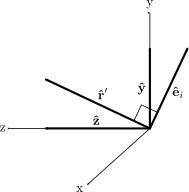
\includegraphics[scale = 1]{Figures/Principios/principios_4}
\caption{Sistema de alineación de vectores para un reflector parabólico.}
\label{fig_principios:4}
\end{figure}
%%%%
La expresión resultante de $\versor{e}_i$, desarrollada en el apéndice \ref{apendice_d}, es:
%%%%
\begin{align}
\versor{e}_i= -\dfrac{\sen^2\theta '\sen\phi '\cos\phi '}{\sqrt{1 - \sen^2\theta '\sen^2\phi '}}\versor{x} + \dfrac{\sen^2\theta '\cos^2\phi ' + \cos^2\theta'}{\sqrt{1 - \sen^2\theta '\sen^2\phi '}}\versor{y} - \dfrac{\sen\theta '\cos\theta '\sen\phi '}{\sqrt{1 - \sen^2\theta '\sen^2\phi '}}\versor{z}
\label{ec_principios:23}
\end{align}
%%%%
A partir de las expresiones \eqref{ec_principios:16} y \eqref{ec_principios:21}, puede demostrarse que en la superficie del reflector:
%%%%
\begin{gather}
\mathbf{J}_s = \dfrac{2}{\eta}\left[\versor{n}\prodvec\left(\versor{s}_i\prodvec\mathbf{E}^i\right)\right] = \dfrac{2}{\eta}\,C_1\sqrt{G_f\left(\theta ',\phi '\right)}\,\frac{e^{-jkr'}}{r'}\,\mathbf{u}
\label{ec_principios:24}\\
\mathbf{u} = \versor{n}\prodvec\left(\versor{r}'\prodvec\versor{e}_i\right) = \left(\versor{n}\prodesc\versor{e}_i\right)\versor{r}' - \left(\versor{n}\prodesc\versor{r}'\right)\versor{e}_i
\tag{\ref{ec_principios:23}a}
\label{ec_principios:25}
\end{gather}
%%%%
y el vector $\mathbf{u}$, cuya expresión fue deducida en el apéndice \ref{apendice_d}, resulta:
%%%%
\begin{align}
\begin{split}
\mathbf{u} &= -\dfrac{\sen\theta '\sen\left(\dfrac{\theta '}{2}\right)\sen\phi '\cos\phi '}{\sqrt{1 - \sen^2\theta '\sen^2\phi '}}\versor{x} + \dfrac{\cos\left(\dfrac{\theta '}{2}\right)\!\left(\cos\theta '\sen^2\phi ' + \cos^2\phi '\right)}{\sqrt{1 - \sen^2\theta '\sen^2\phi '}}\versor{y}\\
&-\dfrac{\cos\theta '\sen\left(\dfrac{\theta '}{2}\right)\sen\phi '}{\sqrt{1 - \sen^2\theta '\sen^2\phi '}}\versor{z}
\label{ec_principios:26}
\end{split}
\end{align}
%%%%
Empleando los potenciales vectoriales $\mathbf{A}$ y $\mathbf{F}$ y utilizando el sistema de coordenadas de la figura \ref{fig_fundamentos:11}, puede demostrarse que los campos $\mathbf{E}$ y $\mathbf{H}$ radiados por las fuentes $\mathbf{J}$ y $\mathbf{M}$ pueden expresarse como \cite{Silver}:
%%%%
\begin{subequations}
\label{grup_ec_principios:2}
\begin{align}
\mathbf{E} &= \mathbf{E}_A + \mathbf{E}_F = -j\frac{1}{4\pi\omega\varepsilon}\int_{V}\!\left[\omega^2\mu\varepsilon\,\mathbf{J} + \gradiente{}\left(\divergencia{\mathbf{J}}\right) - j\omega\varepsilon\rotor{M}\right]\frac{e^{- jkR}}{R}\,dv'
\label{ec_principios:27}\\
\mathbf{H} &= \mathbf{H}_A + \mathbf{H}_F = -j\frac{1}{4\pi\omega\mu}\int_{V}\!\left[\omega^2\mu\varepsilon\,\mathbf{M} + \gradiente{}\left(\divergencia{\mathbf{M}}\right) + j\omega\mu\rotor{J}\right]\frac{e^{- jkR}}{R}\,dv'
\label{ec_principios:28}
\end{align}
\end{subequations}
%%%%
Para observaciones de campo lejano, el operador $\nabla$ puede reemplazarse por \cite{Cheng}:
%%%%
\begin{align}
\nabla = - j\mathbf{k} = -jk\versor{r}
\label{ec_principios:29}
\end{align}
%%%%
y las expresiones \eqref{grup_ec_principios:2} quedan reducidas a:
%%%%
\begin{subequations}
\label{grup_ec_principios:3}
\begin{align}
\mathbf{E} &\simeq -j\frac{1}{4\pi\omega\varepsilon}\int_{V}\!\left[\omega^2\mu\varepsilon\,\mathbf{J} + jk\versor{r}\left(jk\versor{r}\prodesc\mathbf{J}\right) + j\omega\varepsilon jk\versor{r}\prodvec\mathbf{M}\right]\frac{e^{- jkR}}{R}\,dv'
\label{ec_principios:30}\\
\mathbf{H} &\simeq -j\frac{1}{4\pi\omega\mu}\int_{V}\!\left[\omega^2\mu\varepsilon\,\mathbf{M} + jk\versor{r}\left(jk\versor{r}\prodesc\mathbf{M}\right) - j\omega\mu jk\versor{r}\prodvec\mathbf{J}\right]\frac{e^{- jkR}}{R}\,dv'
\label{ec_principios:31}
\end{align}
\end{subequations}
%%%%
Dado que:
%%%%
\begin{align}
k = \omega\sqrt{\varepsilon\mu}
\label{ec_principios:32}
\end{align}
%%%%
las expresiones \eqref{grup_ec_principios:3} resultan:
%%%%
\begin{subequations}
\label{grup_ec_principios:4}
\begin{align}
\mathbf{E} &\simeq -j\frac{\omega\mu}{4\pi r}e^{- jkr}\!\int_{V}\!\left[\mathbf{J} - \left(\mathbf{J}\prodesc\versor{r}\right)\versor{r} - \sqrt{\frac{\varepsilon}{\mu}}\,\versor{r}\prodvec\mathbf{M}\right]\!e^{jk\mathbf{r}'\prodesc\versor{r}}\,dv'
\label{ec_principios:33}\\
\mathbf{H} &\simeq -j\frac{\omega\varepsilon}{4\pi r}e^{- jkr}\!\int_{V}\!\left[\mathbf{M} - \left(\mathbf{M}\prodesc\versor{r}\right)\versor{r} + \sqrt{\frac{\mu}{\varepsilon}}\,\versor{r}\prodvec\mathbf{J}\right]\!e^{jk\mathbf{r}'\prodesc\versor{r}}\,dv'
\label{ec_principios:34}
\end{align}
\end{subequations}
%%%%
Si las distribuciones de corrientes son inducidas por los campos eléctrico y magnético incidentes sobre la superficie $S_1$ mostrada en la figura \ref{fig_principios:3}, los campos creados por estas corrientes se denominan \emph{campos dispersos}. Si la superficie conductora es cerrada, los campos lejanos se obtienen de las ecuaciones \eqref{grup_ec_principios:4} tomando $\mathbf{M} = 0$ y reduciendo la integral de volumen a la integral de superficie con la densidad de corriente superficial $\mathbf{J}$ reemplazada por la densidad de corriente lineal  $\mathbf{J}_s$. Por lo tanto:
\begin{subequations}
\label{grup_ec_principios:5}
\begin{align}
\mathbf{E} &= -j\frac{\omega\mu}{4\pi r}e^{- jkr}\iint\limits_{S_1}\left[\mathbf{J}_s - \left(\mathbf{J}_s\prodesc\versor{r}\right)\versor{r}\right]e^{jk\mathbf{r}'\prodesc\versor{r}}\,ds'
\label{ec_principios:35}\\
\mathbf{H} &= -j\frac{\omega\sqrt{\mu\varepsilon}}{4\pi r}e^{- jkr}\iint\limits_{S_1}\left(\versor{r}\prodvec\mathbf{J}_s\right)e^{jk\mathbf{r}'\prodesc\versor{r}}\,ds'
\label{ec_principios:36}
\end{align}
\end{subequations}
%%%%
La expresión de la densidad de corriente $\mathbf{J}_s$, en términos de sus componentes en coordenadas esféricas, es:
%%%%
\begin{align}
\mathbf{J}_s= {\text{J}_s}_{\text{r}}\,\versor{r} + {\text{J}_s}_{\uptheta}\,\versor{\uptheta} + {\text{J}_s}_{\upphi}\,\versor{\upphi}
\label{ec_principios:37}
\end{align}
%%%%
El término $\mathbf{J}_s$ en el integrando de la expresión \eqref{ec_principios:35} tiene una componente en la dirección $\versor{r}$, pero se cancela con el segundo término $\left(\mathbf{J}_s\prodesc\versor{r}\right)\versor{r}$, porque:
%%%%
\begin{align}
\left(\mathbf{J}_s\prodesc\versor{r}\right)\versor{r}= {\text{J}_s}_{\text{r}}\,\versor{r}
\label{ec_principios:38}
\end{align}
%%%%
Entonces, el campo de la expresión \eqref{ec_principios:35} puede separarse en dos componentes, resultando:
%%%%
\begin{subequations}
\label{grup_ec_principios:6}
\begin{align}
E_{\theta} &= -j\frac{\omega\mu}{4\pi r}e^{- jkr}\!\iint\limits_{S_1}\mathbf{J}_s\prodesc\versor{\uptheta}\,e^{jk\mathbf{r}'\prodesc\versor{r}}ds'
\label{ec_principios:39}\\
E_{\phi} &= -j\frac{\omega\mu}{4\pi r}e^{- jkr}\!\iint\limits_{S_1}\mathbf{J}_s\prodesc\versor{\upphi}\,e^{jk\mathbf{r}'\prodesc\versor{r}}ds'
\label{ec_principios:40}
\end{align}
\end{subequations}
%%%%
Empleando la expresión \eqref{ec_principios:24}, las expresiones \eqref{grup_ec_principios:6} se reducen a:
%%%%
\begin{subequations}
\label{grup_ec_principios:7}
\begin{align}
E_{\theta} &= -j\frac{\omega\mu C_1}{2\eta\pi r}e^{- jkr}\!\iint\limits_{S_1}\!\sqrt{G_f\left(\theta ',\phi '\right)}\,\frac{e^{-jkr'}}{r'}\,\mathbf{u}\prodesc\versor{\uptheta}\,e^{jk\mathbf{r}'\prodesc\versor{r}}ds'
\label{ec_principios:41}\\
E_{\phi} &= -j\frac{\omega\mu C_1}{2\eta\pi r}e^{- jkr}\!\iint\limits_{S_1}\!\sqrt{G_f\left(\theta ',\phi '\right)}\,\frac{e^{-jkr'}}{r'}\,\mathbf{u}\prodesc\versor{\upphi}\,e^{jk\mathbf{r}'\prodesc\versor{r}}ds'
\label{ec_principios:42}
\end{align}
\end{subequations}
%%%%
Dado que $\versor{\uptheta}$ y $\versor{\upphi}$ se expresan como:
%%%%
\begin{subequations}
\label{grup_ec_principios:8}
\begin{align}
\versor{\uptheta} &= \cos\theta\cos\phi\,\versor{x} + \cos\theta\sen\phi\,\versor{y} - \sen\theta\,\versor{z}
\label{ec_principios:43}\\
\versor{\upphi} &= -\sen\phi\,\versor{x} + \cos\phi\,\versor{y}
\label{ec_principios:44}
\end{align}
\end{subequations}
%%%%
$\mathbf{u}\prodesc\versor{\uptheta}$ y $\mathbf{u}\prodesc\versor{\upphi}$, empleando las expresiones \eqref{ec_principios:26} y \eqref{grup_ec_principios:8}, resultan:
%%%%
\begin{subequations}
\label{grup_ec_principios:9}
\begin{align}
\begin{split}
\mathbf{u}\prodesc\versor{\uptheta} &= -\dfrac{\cos\theta\cos\phi\sen\theta '\sen\left(\dfrac{\theta '}{2}\right)\sen\phi '\cos\phi '}{\sqrt{1 - \sen^2\theta '\sen^2\phi '}} + \dfrac{\sen\theta\cos\theta '\sen\left(\dfrac{\theta '}{2}\right)\sen\phi '}{\sqrt{1 - \sen^2\theta '\sen^2\phi '}}\\
&+ \dfrac{\cos\theta\sen\phi\cos\left(\dfrac{\theta '}{2}\right)\!\left(\cos\theta '\sen^2\phi ' + \cos^2\phi '\right)}{\sqrt{1 - \sen^2\theta '\sen^2\phi '}}
\label{ec_principios:45}
\end{split}\\
\mathbf{u}\prodesc\versor{\upphi} &= \dfrac{\sen\phi\sen\theta '\sen\left(\dfrac{\theta '}{2}\right)\sen\phi '\cos\phi '}{\sqrt{1 - \sen^2\theta '\sen^2\phi '}} + \dfrac{\cos\phi\cos\left(\dfrac{\theta '}{2}\right)\!\left(\cos\theta '\sen^2\phi ' + \cos^2\phi '\right)}{\sqrt{1 - \sen^2\theta '\sen^2\phi '}}
\label{ec_principios:46}
\end{align}
\end{subequations}
%%%%
La expresión de $\mathbf{r}'\prodesc\versor{r}$ es \cite{Balanisantenas}:
%%%%
\begin{align}
\mathbf{r}'\prodesc\versor{r} = r'\left[\sen\theta\sen\theta '\cos\left(\phi - \phi '\right) + \cos\theta\cos\theta '\right]
\label{ec_principios:47}
\end{align}
%%%%
\begin{figure} [H]
\centering 
\subfigure[Proyección del área.]{
\label{fig_principios:5}
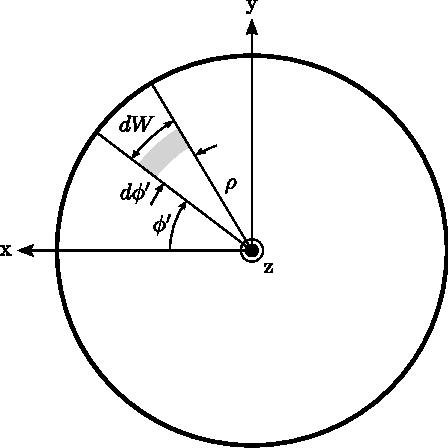
\includegraphics[scale = 1]{Figures/Principios/principios_5.pdf}}
\subfigure[Vista lateral.]{
\label{fig_principios:6}
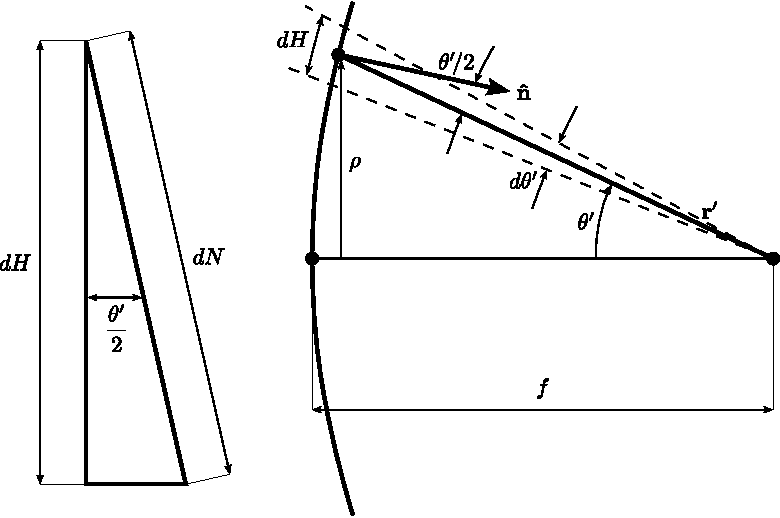
\includegraphics[scale = 1]{Figures/Principios/principios_6.pdf}}
\caption{Proyección del área y vista lateral del reflector.}
\label{grup_fig_principios:1}
\end{figure}
%%%%
De acuerdo a la geometría de la figura \ref{grup_fig_principios:1}:
%%%%
\begin{align}
ds' = dWdN = \left(r'\sen\theta 'd\phi '\right)\!\left[r'\sec\left(\frac{\theta '}{2}\right)\!d\theta '\right] = {r'}^2\sen\theta '\sec\left(\frac{\theta '}{2}\right)\!d\theta 'd\phi '
\label{ec_principios:48}
\end{align}
%%%%
donde:
%%%%%
\begin{align}
dW &= r'\sen\theta 'd\phi'
\tag{\ref{ec_principios:48}a}
\label{ec_principios:49}\\
\begin{split}
dH &= -\versor{r}\prodesc d\mathbf{N} = -\versor{r}\prodesc\versor{n}\,dN\\
&= -\versor{r}\prodesc\left[-\cos\left(\frac{\theta '}{2}\right)\!\versor{r} + \sen\left(\frac{\theta '}{2}\right)\!\versor{\uptheta}\right]\!dN = \cos\left(\frac{\theta '}{2}\right)\!dN
\end{split}
\tag{\ref{ec_principios:48}b}
\label{ec_principios:50}\\
dN &= \sec\left(\frac{\theta '}{2}\right)\!dH = \sec\left(\frac{\theta '}{2}\right)\!r'd\theta ' = r'\sec\left(\frac{\theta '}{2}\right)\!d\theta '
\tag{\ref{ec_principios:48}c}
\label{ec_principios:51}
\end{align}
%%%%
Empleando las expresiones \eqref{ec_principios:2}, \eqref{grup_ec_principios:9}, \eqref{ec_principios:47} y \eqref{ec_principios:48}, las expresiones de los campos \eqref{grup_ec_principios:7} quedan reducidas a:
%%%%
\begin{subequations}
\label{grup_ec_principios:10}
\begin{align}
E_{\theta} &= -j\frac{\omega\mu FC_1}{2\eta\pi r}e^{- jkr}\left(-\cos\theta\cos\phi\,\mathbf{I}_1 + \cos\theta\sen\phi\,\mathbf{I}_2 + \sen\theta\,\mathbf{I}_3\right)
\label{ec_principios:52}\\
E_{\phi} &= -j\frac{\omega\mu FC_1}{2\eta\pi r}e^{- jkr}\left(\sen\phi\,\mathbf{I}_1 + \cos\phi\mathbf{I}_2\right)
\label{ec_principios:53}
\end{align}
\end{subequations}
%%%%
donde:
%%%%
\begin{subequations}
\label{grup_ec_principios:11}
\begin{align}
\begin{split}
\mathbf{I}_1 &= \!\!\bigint_{\phi ' = 0}^{2\pi}\!\!\bigint_{\theta ' = 0}^{\theta_0}\!\!\!\!\!\sqrt{G_f\left(\theta ',\phi '\right)}\,\dfrac{\sen^2\theta '\sen\left(\dfrac{\theta '}{2}\right)\sen\phi '\cos\phi '}{\cos^3\left(\dfrac{\theta '}{2}\right)\!\sqrt{1 - \sen^2\theta '\sen^2\phi '}}\\
&\times e^{-jkF\left[1 - \sen\theta\sen\theta '\cos\left(\phi - \phi '\right) - \cos\theta\cos\theta '\right]/\cos^2\left(\frac{\theta '}{2}\right)}d\theta 'd\phi '
\end{split}
\label{ec_principios:54}\\
\begin{split}
\mathbf{I}_2 &= \!\!\bigint_{\phi ' = 0}^{2\pi}\!\!\bigint_{\theta ' = 0}^{\theta_0}\!\!\!\!\!\sqrt{G_f\left(\theta ',\phi '\right)}\,\dfrac{\sen\theta '\left[\cos\theta '\sen^2\phi ' + \cos^2\phi '\right]}{\cos^2\left(\dfrac{\theta '}{2}\right)\!\sqrt{1 - \sen^2\theta '\sen^2\phi '}}\\
&\times e^{-jkF\left[1 - \sen\theta\sen\theta '\cos\left(\phi - \phi '\right) - \cos\theta\cos\theta '\right]/\cos^2\left(\frac{\theta '}{2}\right)}d\theta 'd\phi '
\end{split}
\label{ec_principios:55}\\
\begin{split}
\mathbf{I}_3 &= \!\!\bigint_{\phi ' = 0}^{2\pi}\!\!\bigint_{\theta ' = 0}^{\theta_0}\!\!\!\!\!\sqrt{G_f\left(\theta ',\phi '\right)}\,\dfrac{\sen\theta '\cos\theta '\sen\left(\dfrac{\theta '}{2}\right)\sen\phi '}{\cos^3\left(\dfrac{\theta '}{2}\right)\!\sqrt{1 - \sen^2\theta '\sen^2\phi '}}\\
&\times e^{-jkF\left[1 - \sen\theta\sen\theta '\cos\left(\phi - \phi '\right) - \cos\theta\cos\theta '\right]/\cos^2\left(\frac{\theta '}{2}\right)}d\theta 'd\phi '
\end{split}
\label{ec_principios:56}
\end{align}
\end{subequations}
%%%%

%%%%
\section{Ganancia y eficiencia de abertura}
\label{sec_principios_gan_ef_abertura}
%%%%

%%%%
En la sección \ref{subsec_intro_area_efec}, se dedujo que la ganancia de una antena puede expresarse como:
%%%%
\begin{align}
G_0 = \dfrac{4\pi}{\lambda^2}A_{em}
\label{ec_principios:57}
\end{align}
%%%%
y empleando la expresión \eqref{ec_intro:54}, $G_0$ queda expresada como:
%%%%
\begin{align}
G_0 = \dfrac{4\pi}{\lambda^2}\varepsilon_{ap}A_p
\label{ec_principios:58}
\end{align}
%%%%
Conociendo la longitud de onda y el área de la superficie física $A_p$, el estudio de la ganancia se reduce a la determinación de la eficiencia de abertura $\varepsilon_{ap}$, la cual puede ser expresada como:
%%%%
\begin{align}
\varepsilon_{ap} = e_r\varepsilon_t\varepsilon_s\varepsilon_o
\label{ec_principios:59}
\end{align}
%%%%
donde:
%%%%
\begin{align*}
e_r = &\text{ Eficiencia de radiación, debida a pérdidas óhmicas.}\\
\varepsilon_t = &\text{ Eficiencia\hspace{0.43mm} de\hspace{0.43mm} iluminación,\hspace{0.43mm} debida\hspace{0.43mm} a\hspace{0.43mm} la\hspace{0.43mm} distribución\hspace{0.43mm} de\hspace{0.43mm} amplitud\hspace{0.43mm} no\hspace{0.43mm} uniforme\hspace{0.43mm} del}\\
&\text{ diagrama de radiación del alimentador sobre la superficie del reflector.}\\
\varepsilon_s = &\text{ Eficiencia\hspace{0.43mm} por\hspace{0.43mm} spillover,\hspace{0.43mm} debida\hspace{0.43mm} a\hspace{0.43mm} la\hspace{0.43mm} fracción\hspace{0.43mm} de\hspace{0.43mm} la\hspace{0.43mm} potencia\hspace{0.43mm} total\hspace{0.43mm} radiada\hspace{0.43mm} por\hspace{0.43mm} el}\\
&\text{ alimentador dentro del ángulo de abertura del reflector $\theta_0$.}\\
\varepsilon_o = &\text{ Eficiencias debidas a otros factores.}
\end{align*}
%%%%
Combinando las eficiencias $\varepsilon_t$ y $\varepsilon_s$, se obtiene la \emph{eficiencia global de iluminación} $\varepsilon_i$.

%%%%
\subsection{Eficiencia global de iluminación}
\label{subsec_principios_efi_glo_ilu}
%%%%

La expresión de la eficiencia de iluminación $\varepsilon_t$ fue deducida previamente en la sección \ref{sec_fundamentos_area_ef_ant_aber}. Para un reflector parabólico de radio $a$, la expresión \eqref{ec_fundamentos:94} se reduce a:
%%%%
\begin{align}
\varepsilon_t  = \dfrac{1}{\pi a^2}\dfrac{\left|\displaystyle\int_0^{2\pi}\!\!\!\int_0^a\lvert\mathbf{E}_a\rvert\, ds'\right|^2}{\displaystyle\int_0^{2\pi}\!\!\!\int_0^a\lvert\mathbf{E}_a\rvert^2 ds'}
\label{ec_principios:60}
\end{align}
%%%%
La potencia radiada por el alimentador dentro del ángulo sólido $d\Omega ' = \sen\theta 'd\theta 'd\phi '$ debe ser igual a la potencia incidente sobre el reflector parabólico que se propaga paralela al eje \emph{z} a través de la superficie $ds' = \rho 'd\rho 'd\phi '$ \cite{Orfanidis}. Dado que $ \lvert\mathbf{E_a}\rvert ^2/2\eta$ es la densidad de potencia del campo sobre la abertura y asumiendo que $U_f\left(\theta ',\phi '\right)$ es la intensidad de radiación del alimentador, a partir de las condiciones de potencia surge la relación:
%%%%
\begin{align}
\dfrac{1}{2\eta}\lvert\mathbf{E_a}\rvert ^2ds' = U_f\left(\theta ',\phi '\right)\!d\Omega '\Longrightarrow \dfrac{1}{2\eta}\lvert\mathbf{E_a}\rvert ^2\rho 'd\rho ' = U_f\left(\theta ',\phi '\right)\sen\theta 'd\theta '
\label{ec_principios:61}
\end{align}
%%%%
Derivando la expresión \eqref{ec_principios:3}, se obtiene:
%%%%
\begin{align}
\dfrac{d\rho '}{d\theta '} = \dfrac{F}{\cos^2\theta '}
\label{ec_principios:62}
\end{align}
%%%%
y empleando las expresiones \eqref{ec_principios:2} y \eqref{ec_principios:62}, se llega a:
%%%%
\begin{align}
d\rho ' = r'd\theta '
\label{ec_principios:63}
\end{align}
%%%%
A partir de las expresiones \eqref{ec_principios:3} y \eqref{ec_principios:63}, se obtiene:
%%%%
\begin{align}
\rho 'd\rho ' = {r'}^2\sen\theta 'd\theta ' = r'2F\tan\left(\frac{\theta '}{2}\right)d\theta '
\label{ec_principios:64}
\end{align}
%%%%
Empleando las expresiones \eqref{ec_principios:61} y \eqref{ec_principios:64}, se obtienen las relaciones:
%%%%
\begin{subequations}
\label{grup_ec_principios:12}
\begin{align}
\lvert\mathbf{E_a}\rvert ^2 &= \dfrac{2\eta\,U_f\left(\theta ',\phi '\right)}{{r'}^2}
\label{ec_principios:65}\\
\lvert\mathbf{E_a}\rvert &= \dfrac{\sqrt{2\eta\,U_f\left(\theta ',\phi '\right)}}{r'}
\label{ec_principios:66}
\end{align}
\end{subequations}
%%%%
y relacionando las expresiones \eqref{ec_principios:64} y \eqref{grup_ec_principios:12}, se llega a:
%%%%
\begin{subequations}
\label{grup_ec_principios:13}
\begin{align}
\lvert\mathbf{E_a}\rvert ^2ds' &= \lvert\mathbf{E_a}\rvert ^2\rho 'd\rho 'd\phi ' = 2\eta\,U_f\left(\theta ',\phi '\right)\sen\theta 'd\theta 'd\phi '
\label{ec_principios:67}\\
\lvert\mathbf{E_a}\rvert ds' &= \lvert\mathbf{E_a}\rvert \rho 'd\rho 'd\phi ' = 2F\sqrt{2\eta\,U_f\left(\theta ',\phi '\right)}\tan\left(\frac{\theta '}{2}\right)\!d\theta 'd\phi '
\label{ec_principios:68}
\end{align}
\end{subequations}
%%%%
Empleando las expresiones \eqref{ec_principios:60} y \eqref{grup_ec_principios:13}, la eficiencia de iluminación queda expresada como:
%%%%
\begin{align}
\varepsilon_t  = \dfrac{4F^2}{\pi a^2}\dfrac{\left|\displaystyle\int_0^{2\pi}\!\!\!\int_0^{\theta_0}\! \sqrt{\,U_f\left(\theta ',\phi '\right)}\tan\left(\frac{\theta '}{2}\right)\!d\theta 'd\phi '\right|^2}{\displaystyle\int_0^{2\pi}\!\!\!\int_0^{\theta_0}U_f\left(\theta ',\phi '\right)\sen\theta 'd\theta 'd\phi '}
\label{ec_principios:69}
\end{align}
%%%%
Considerando que $a = D/2$ y normalizando la intensidad de radiación del alimentador $U_f$, la expresión \eqref{ec_principios:69} se reduce a:
%%%%
\begin{align}
\varepsilon_t  = \dfrac{16F^2}{\pi D^2}\dfrac{\left|\displaystyle\int_0^{2\pi}\!\!\!\int_0^{\theta_0}\! \sqrt{\,F_{nf}\left(\theta ',\phi '\right)}\tan\left(\frac{\theta '}{2}\right)\!d\theta 'd\phi '\right|^2}{\displaystyle\int_0^{2\pi}\!\!\!\int_0^{\theta_0}F_{nf}\left(\theta ',\phi '\right)\sen\theta 'd\theta 'd\phi '}
\label{ec_principios:70}
\end{align}
%%%%
donde $F_{nf}$ es el factor de diagrama de potencia normalizado del alimentador, cuya relación con la intensidad de radiación fue deducida en la sección \ref{subsec_intro_direc}.

Finalmente, introduciendo la expresión \eqref{ec_principios:4}, $\varepsilon_t$ queda expresada como:
%%%%
\begin{align}
\varepsilon_t  = \dfrac{1}{\pi}\cot^2\left(\frac{\theta_0}{2}\right)\dfrac{\left|\displaystyle\int_0^{2\pi}\!\!\!\int_0^{\theta_0}\! \sqrt{\,F_{nf}\left(\theta ',\phi '\right)}\tan\left(\frac{\theta '}{2}\right)\!d\theta 'd\phi '\right|^2}{\displaystyle\int_0^{2\pi}\!\!\!\int_0^{\theta_0}F_{nf}\left(\theta ',\phi '\right)\sen\theta 'd\theta 'd\phi '}
\label{ec_principios:71}
\end{align}
%%%%
Por definición, la eficiencia por spillover $\varepsilon_s$ es la relación entre la potencia captada por el reflector respecto a la potencia total radiada por el alimentador, por lo que puede expresarse como:
%%%%
\begin{align}
\varepsilon_s  = \dfrac{\displaystyle\int_0^{2\pi}\!\!\!\int_0^{\theta_0}F_{nf}\left(\theta ',\phi '\right)\sen\theta 'd\theta 'd\phi '}{\displaystyle\int_0^{2\pi}\!\!\!\int_0^{\pi}F_{nf}\left(\theta ',\phi '\right)\sen\theta 'd\theta 'd\phi '}
\label{ec_principios:72}
\end{align}
%%%%
Combinando las eficiencias $\varepsilon_t$ y $\varepsilon_s$ y asumiendo condiciones ideales en las que no existen pérdidas óhmicas ($e_r = 1$) y debidas a otros factores ($\varepsilon_o = 1$), la eficiencia de abertura $\varepsilon_{ap}$ queda expresada como:
%%%%
\begin{align}
\varepsilon_{ap}  = \varepsilon_i = \varepsilon_t\varepsilon_s = \dfrac{1}{\pi}\cot^2\left(\frac{\theta_0}{2}\right)\dfrac{\left|\displaystyle\int_0^{2\pi}\!\!\!\int_0^{\theta_0}\! \sqrt{\,F_{nf}\left(\theta ',\phi '\right)}\tan\left(\frac{\theta '}{2}\right)\!d\theta 'd\phi '\right|^2}{\displaystyle\int_0^{2\pi}\!\!\!\int_0^{\pi}F_{nf}\left(\theta ',\phi '\right)\sen\theta 'd\theta 'd\phi '}
\label{ec_principios:73}
\end{align}
%%%%
donde $\varepsilon_i$ es la \emph{eficiencia global de iluminación}.

Empleando las expresiones \eqref{ec_intro:20} - \eqref{ec_intro:22}, la expresión \eqref{ec_principios:73} se reduce a:
%%%%
\begin{align}
\varepsilon_{ap}  = \dfrac{1}{4\pi ^2}\cot^2\left(\frac{\theta_0}{2}\right)\left|\displaystyle\int_0^{2\pi}\!\!\!\int_0^{\theta_0}\! \sqrt{\,G_f\left(\theta ',\phi '\right)}\tan\left(\frac{\theta '}{2}\right)\!d\theta 'd\phi '\right|^2
\label{ec_principios:74}
\end{align}
%%%%
donde $G_f$ es la ganancia del alimentador. Con el fin de facilitar el análisis de la eficiencia de abertura, se asume que el diagrama de radiación del alimentador posee simetría rotacional (o sea, no es función del ángulo $\upphi$'), por lo que la expresión \eqref{ec_principios:74} queda reducida a:
%%%%
\begin{align}
\varepsilon_{ap}  = \cot^2\left(\frac{\theta_0}{2}\right)\left|\displaystyle\int_0^{\theta_0}\! \sqrt{\,G_f\left(\theta '\right)}\tan\left(\frac{\theta '}{2}\right)\!d\theta '\right|^2
\label{ec_principios:75}
\end{align}
%%%%
Para lograr la máxima eficiencia de abertura, el diagrama de radiación del alimentador debería ser como el de la figura \ref{fig_principios:7}. Puede observarse que la radiación está concentrada dentro del ángulo de abertura $\theta_0$, cayendo abruptamente fuera de dicho ángulo, logrando así una $\epsilon_s = 1$. A la vez, la radiación es mayor en el ángulo $\theta_0$ que en dirección hacia el vértice del reflector, logrando así una iluminación uniforme sobre la superficie del reflector y obteniendo una $\epsilon_t = 1$. Sin embargo, los diagramas de radiación obtenidos en la práctica son más similares a los de la figura \ref{fig_principios:8}.
%%%%
\begin{figure} [H]
\centering 
\subfigure[Alimentador ideal.]{
\label{fig_principios:7}
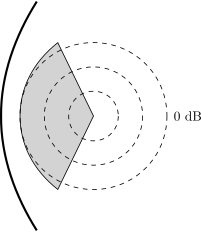
\includegraphics[scale = 1]{Figures/Principios/principios_7}}
\hspace{5mm}
\subfigure[Alimentador real.]{
\label{fig_principios:8}
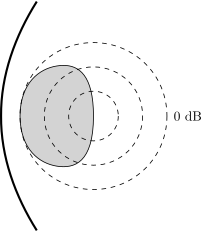
\includegraphics[scale = 1]{Figures/Principios/principios_8}}
\caption{Diagramas de radiación de alimentadores.}
\label{grup_fig_principios:2}
\end{figure}
%%%%
Cualquier alimentador en la práctica producirá pérdidas por \emph{iluminación no uniforme} y por \emph{spillover}, como puede verse en la figura \ref{fig_principios:9}. Un diagrama de radiación más delgado mejora $\epsilon_s$ pero empeora $\epsilon_t$, mientras que uno más ancho mejora $\epsilon_t$ pero empeora $\epsilon_s$.
%%%%
\begin{figure}[H]
\centering
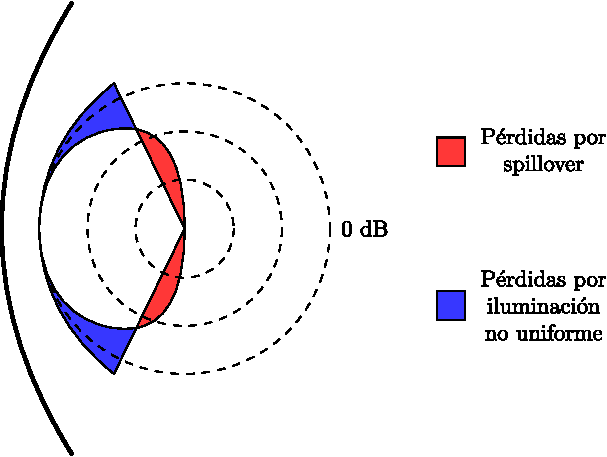
\includegraphics[scale = 01]{Figures/Principios/principios_9}
\caption{Pérdidas en la iluminación de un reflector parabólico.}
\label{fig_principios:9}
\end{figure}
%%%%
\emph{El problema del diseño del alimentador se reduce entonces a una solución de compromiso que permita obtener una} $\epsilon_s$ \emph{y una} $\epsilon_t$ \emph{tales que la eficiencia de abertura} $\epsilon_{ap}$ \emph{sea máxima}.

Para demostrar la variación de la eficiencia de abertura en función del ángulo $\theta_0$ y de la relación $F/D$, Silver \cite{Silver} consideró un tipo de alimentador cuyo diagrama de radiación está definido por:
%%%%
\begin{align}
G_f\left(\theta '\right) = 
\begin{cases} 
{G_0}^{\left(n\right)}\cos^n\left(\theta '\right)  &\mbox{si}\;0\leq\theta '\leq\pi/2\\
0  &\text{si}\;\pi/2\leq\theta '\leq\pi
\end{cases}
\label{ec_principios:76}
\end{align}
%%%%
donde ${G_0}^{\left(n\right)}$ es una constante dada por el valor $n$. Aunque son ideales, estos diagramas de radiación se escogieron porque permiten obtener expresiones cerradas y porque generalmente permiten obtener una buena representación del lóbulo principal en la práctica. La radiación directa del alimentador ($\uptheta$' $> \pi/2$) se asume nula con el fin de evitar la interferencia con la radiación reflejada.

A partir de la relación:
%%%%
\begin{align}
\iint\limits_{S}G_f\left(\theta '\right)\!d\Omega ' = \iint\limits_{S}G_f\left(\theta '\right)\sen\theta 'd\theta 'd\phi ' = 4\pi
\label{ec_principios:77}
\end{align}
%%%%
se determina la constante ${G_0}^{\left(n\right)}$:
%%%%
\begin{align}
{G_0}^{\left(n\right)}\!\int_0^{\,\pi /2}\!\cos^n\theta '\sen\theta 'd\theta ' = 2 \Longrightarrow {G_0}^{\left(n\right)} = 2\left(n + 1\right)
\label{ec_principios:78}
\end{align}
%%%%
por lo que la expresión \eqref{ec_principios:76} se reduce a:
%%%%
\begin{align}
G_f\left(\theta '\right) = 
\begin{cases} 
2\left(n + 1\right)\cos^n\left(\theta '\right)  &\mbox{si}\;0\leq\theta '\leq\pi/2\\
0  &\text{si}\;\pi/2\leq\theta '\leq\pi
\end{cases}
\label{ec_principios:79}
\end{align}
%%%%
La expresión \eqref{ec_principios:75}, para valores pares de $n$ comprendidos entre 2 y 8 y empleando la expresión \eqref{ec_principios:79}, resulta:
%%%%
\begin{subequations}
\label{grup_ec_principios:14}
\begin{align}
\epsilon_{ap}\left(n = 2\right) &= 24\left\{\sen^2\left(\frac{\theta_0}{2}\right) + \ln\left[\cos\left(\frac{\theta_0}{2}\right)\right]\right\}^2\!\cot^2\left(\frac{\theta_0}{2}\right)
\label{ec_principios:80}\\
\epsilon_{ap}\left(n = 4\right) &= 40\left\{\sen^4\left(\frac{\theta_0}{2}\right) + \ln\left[\cos\left(\frac{\theta_0}{2}\right)\right]\right\}^2\!\cot^2\left(\frac{\theta_0}{2}\right)
\label{ec_principios:81}\\
\epsilon_{ap}\left(n = 6\right) &= 14\left\{2\ln\left[\cos\left(\frac{\theta_0}{2}\right)\right] + \frac{\left(1 - \cos\theta_0\right)^3}{3} + \frac{1}{2}\sen^2\theta_0\right\}^2\!\cot^2\left(\frac{\theta_0}{2}\right)
\label{ec_principios:82}\\
\begin{split}
\epsilon_{ap}\left(n = 8\right) &= 18\left\{\frac{1 - \cos^4\theta_0}{4} - 2\ln\left[\cos\left(\frac{\theta_0}{2}\right)\right] - \frac{\left(1 - \cos\theta_0\right)^3}{3}\right.\\
&\left.- \frac{1}{2}\sen^2\theta_0\right\}^2\!\cot^2\left(\frac{\theta_0}{2}\right)
\end{split}
\label{ec_principios:83}
\end{align}
\end{subequations}
%%%%
Las variaciones de la eficiencia de abertura $\epsilon_{ap}$ en función del ángulo de abertura $\theta_0$ o de la relación $F/D$ para distintos valores de \emph{n} pueden verse en la figura \ref{fig_principios:10}.
%%%%
\begin{figure}[H]
\centering
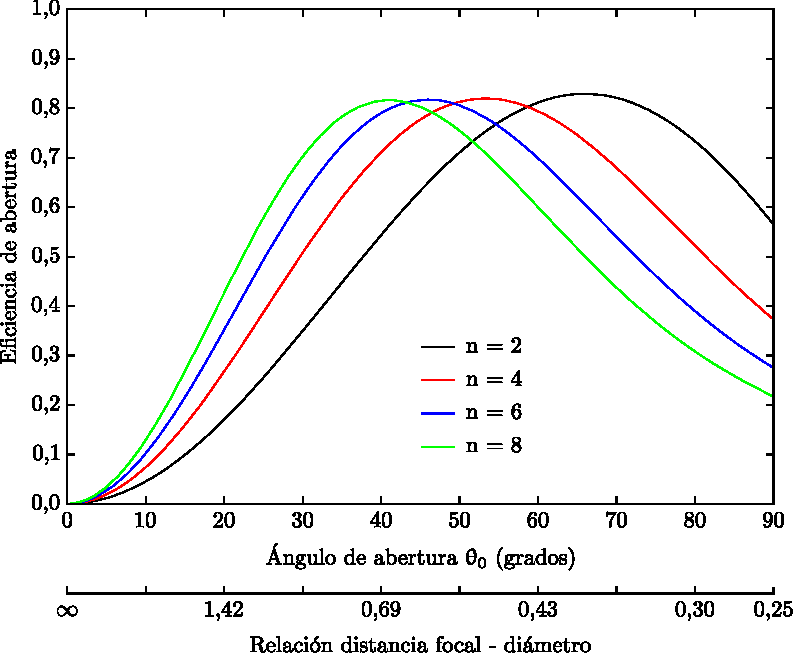
\includegraphics[scale = 0.98]{Figures/Principios/principios_10}
\caption{Eficiencia de abertura en función del ángulo $\theta_0$ (o de la relación $F/D$).}
\label{fig_principios:10}
\end{figure}
%%%%
Valiéndose de la figura \ref{fig_principios:11}, para cada valor de $n$ se analiza la diferencia entre las potencias incidentes en el borde y el vértice del reflector $EI$, cuya expresión es:
%%%%
\begin{align}
EI_{dB} = 10\log\left(G_{fn}\left(\theta_0\right)\right) + P\!A
\label{ec_principios:84}
\end{align}
%%%%
donde $G_{fn}\left(\theta '\right)$ corresponde a la ganancia normalizada del alimentador dado por la expresión \eqref{ec_principios:79} y $P\!A$ es la atenuación en el espacio libre producida en la diferencia de caminos $\Delta r$ que se expresa como:
%%%%
\begin{align}
P\!A_{dB} = 20\log\left(\dfrac{F}{r_0}\right)
\label{ec_principios:85}
\end{align}
%%%%
\begin{figure}[H]
\centering
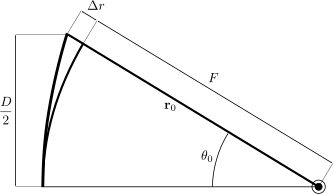
\includegraphics[scale = 1]{Figures/Principios/principios_11}
\caption{Iluminación en el borde y en el vértice del reflector.}
\label{fig_principios:11}
\end{figure}
%%%%
Aplicando propiedades trigonométricas, la expresión \eqref{ec_principios:85} se reduce a:
%%%%
\begin{align}
P\!A_{dB} = 20\log\left(2\,\dfrac{F}{D}\sen\theta_0\right)
\label{ec_principios:86}
\end{align}
%%%%
En la tabla \ref{tabla_principios:1} pueden observarse los resultados obtenidos para los valores de $n$ comprendidos entre 2 y 8.
%%%%
\begin{table}[H]
\centering
\begin{tabular}{|c|c|c|c|c|c|c|c|c|}
\hline
n & $\epsilon_s$ & $\epsilon_t$ & $\epsilon_{ap}$ & $\theta_0\,$(grados) & $F/D$ & $G_{fn}\left(\theta_0\right)\,$(dB) & $P\!A\,$(dB) & $EI\,$(dB)\\
\hline
2 & 0,933 & 0,889 & 0,829 & 60,0 & 0,385 & -7,810 & -3,055 & -10,865\\
\hline
4 & 0,924 & 0,887 & 0,820 & 53,3 & 0,498 & -8,946 & -1,952 & -10,898\\
\hline
6 & 0,921 & 0,887 & 0,817 & 45,9 & 0,590 & -9,470 & -1,436 & -10,906\\
\hline
8 & 0,920 & 0,887 & 0,816 & 41,0 & 0,669 & -9,772 & -1,136 & -10,908\\
\hline
\end{tabular}
\caption{Eficiencias de abertura y diferencias entre las potencias incidentes en el borde y el vértice del reflector para distintos valores de $n$.}
\label{tabla_principios:1}
\end{table}
%%%%
Los valores de $EI$ para los casos analizados son aproximadamente -11 dB, y la eficiencia de abertura se encuentra en torno al 82 \%. Entonces, puede decirse que \emph{la eficiencia de abertura en términos de iluminación es máxima cuando la diferencia entre las potencias incidentes en el borde y en el vértice del reflector es de -11 dB}. Esta es la solución de compromiso a partir de la cual se debe diseñar el alimentador.

%%%%
\subsection{Otras eficiencias}
\label{subsec_principios_otras_efi}
%%%%

La eficiencia de abertura se debe, además de al patrón de iluminación del reflector, a otros grupo de factores; se define entonces a la \emph{eficiencia debida a otros factores} $\varepsilon_o$ como:
%%%%
\begin{align*}
\varepsilon_o = \varepsilon_p\varepsilon_b\varepsilon_x
\end{align*}
%%%%
donde:
%%%%
\begin{enumerate}
\item \emph{Eficiencia de fase $\varepsilon_p$}, debida a la no uniformidad de la fase del campo sobre el plano de abertura.
\item \emph{Eficiencia por bloqueo $\varepsilon_b$}, debida al bloqueo parcial del campo reflejado producido por el alimentador.
\item \emph{Eficiencia por polarización cruzada $\varepsilon_x$}, debida a la existencia de campos con polariación cruzada sobre el plano de abertura.
\end{enumerate}
%%%%
Existen otros factores que inciden en la eficiencia de abertura, como las irregularidades en la superficie del reflector y los desplazamientos axiales y laterales del alimentador respecto de su ubicación en el foco, pero se desprecian con el fin de facilitar el estudio de $\varepsilon_{ap}$.

La expresión de la eficiencia de fase $\varepsilon_p$ fue deducida previamente en la sección \ref{sec_fundamentos_area_ef_ant_aber}. Empleando el mismo análisis utilizado para deducir la eficiencia de iluminación global $\varepsilon_i$, la expresión \eqref{ec_fundamentos:95} se reduce a:
%%%%
\begin{align}
\varepsilon_p  = \dfrac{\left|\displaystyle\int_0^{2\pi}\!\!\!\int_0^{\theta_0}\! \sqrt{\,F_{nf}\left(\theta ',\phi '\right)}\,e^{-jk\delta}\tan\left(\frac{\theta '}{2}\right)\!d\theta 'd\phi '\right|^2}{\left|\displaystyle\int_0^{2\pi}\!\!\!\int_0^{\theta_0}\! \sqrt{\,F_{nf}\left(\theta ',\phi '\right)}\tan\left(\frac{\theta '}{2}\right)\!d\theta 'd\phi '\right|^2}
\label{ec_principios:87}
\end{align}
%%%%
donde el término $e^{-jk\delta}$ representa la variación de fase de los campos sobre el plano de abertura, y $\delta$ depende directamente de las características de radiación del alimentador.

En la sección \ref{sec_principios_intro} se determinó que si el centro de fase del alimentador coincide con el foco del reflector parabólico, la fase a través del plano de abertura será uniforme. Entonces, \emph{una característica deseable del alimentador es que su centro de fase coincida con el foco del reflector}, en cuyo caso $\delta = 0$ y la eficiencia de fase $\varepsilon_p = 1$. Muchas veces no es posible obtener un alimentador que cumpla tal característica; en tal caso, el alimentador tendrá un cierto \emph{error de fase}, el cual deberá ser lo menor posible para que $\varepsilon_p$ sea máxima.

La eficiencia por bloqueo $\varepsilon_b$ depende directamente de las dimensiones del alimentador, y puede determinarse aproximadamente a partir de la expresión \cite{Stutzman}:
%%%%
\begin{align}
\varepsilon_b  = \left(1 - \dfrac{1}{\varepsilon_t}\dfrac{A_f}{A_p}\right)^2
\label{ec_principios:88}
\end{align}
%%%%
donde $A_f$ es el área de bloqueo proyectada por el alimentador y $A_p$ es el área proyectada del reflector parabólico.

Dado que en la medida que se incrementen las dimensiones del alimentador disminuye $\varepsilon_b$, \emph{otra característica deseable del alimentador es que sus dimensiones sean lo menor posible}.

La eficiencia por polarización cruzada $\varepsilon_x$ se debe a contribuciones del alimentador, ya que los reflectores parabólicos de foco centrado no introducen componentes contrapolares. La mayoría de las veces puede despreciarse, fundamentalmente considerando que la polarización cruzada es prácticamente nula en la dirección de propagación principal $\left(\uptheta = 0^{\circ}\right)$. En la sección \ref{sec_polarizacion_cruzada} se analizará más en detalle la polarización cruzada generada por una antena parabólica.

%%%%
\section{Polarización cruzada}
\label{sec_polarizacion_cruzada}
%%%%

Para el estudio de la polarización cruzada en un reflector parabólico, se considera inicialmente que el alimentador está linealmente polarizado a lo largo del eje \emph{y}. Si el diagrama de radiación del alimentador tuviera simetría rotacional, es decir, si fuera solamente función de $\uptheta$' y no de $\upphi$', la componente contrapolar de los campos radiados por el reflector parabólico sería nula. Puede decirse entonces que en una antena parabólica de foco centrado \emph{la existencia de componentes contrapolares del campo se debe exclusivamente a contribuciones del alimentador} \cite{Stutzman}.

Es deseable, por lo tanto, que un alimentador tenga las siguientes características:
\begin{itemize}
\item Baja polarización cruzada.
\item Diagrama de radiación con la mayor simetría rotacional posible.
\end{itemize}
%%%%
A partir de los campos radiados por el reflector \eqref{grup_ec_principios:10}, se determinan las componentes $E_x$ y $E_y$, donde $E_y$ corresponde a la copolarización y $E_x$ a la polarización cruzada. La componente contrapolar es nula para los planos \emph{E} ($\upphi = 90^{\circ}$) y \emph{H} ($\upphi = 0^{\circ}$) y máxima para el plano $\upphi = 45^{\circ}$; además, disminuye en la medida que la relación $F/D$ aumente \cite{Stutzman} \cite{Collin}. En la figura \ref{fig_principios:12} puede observarse como varía comúnmente la copolarización y la polarización cruzada de una antena parabólica de foco centrado en función del ángulo $\uptheta$, para el plano $\upphi = 45^{\circ}$.
%%%%
\begin{figure}[H]
\centering
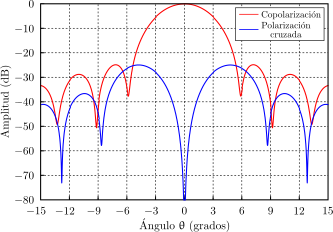
\includegraphics[scale = 1]{Figures/Principios/principios_12}
\caption{Copolarización y polarización cruzada de una antena parabólica de foco centrado, para el plano $\upphi = 45^{\circ}$.}
\label{fig_principios:12}
\end{figure}
%%%%

\chapter{Estudio y diseño de metamteriales}
\label{cap_estudio}
\lhead{Capítulo \ref{cap_estudio}. \emph{Estudio y diseño del alimentador}}
%%%%%%%%%%%%%%%%%%%%%%%
%%  Capítulo 4: Estudio y diseño de la antena  %%
%%%%%%%%%%%%%%%%%%%%%%%

%%%%
\section{Parámetros de iluminación del reflector}
\label{sec_estudio_param}
%%%%

Para definir la antena que será utilizada como alimentador y sus respectivas dimensiones, es necesario en primer lugar conocer las dimensiones del reflector parabólico para poder determinar el diagrama de radiación del alimentador que se ajuste a lo pedido: EI = -11 dB, como se explicó en la sección \ref{subsec_principios_efi_glo_ilu}.

Las dimensiones del reflector parabólico son:
%%%%
\begin{align*}
D &= \text{1,8 m}\\
F &= \text{63,6 cm}\\
h_0 &= \text{31,8 cm}\\
r_0 &= \text{95,5 cm}\\
\theta_0 &= \text{71,5}^{\circ}\\
\dfrac{F}{D} &= \text{0,353}
\end{align*}
%%%%
A partir de la expresión \eqref{ec_principios:84}, la ganancia normalizada en dB en el ángulo $\theta_0$ queda expresada como:
%%%%
\begin{align}
{G_{fn}\left(\theta_0\right)}_{dB} = -11 \text{ dB} - P\!A
\label{ec_estudio:1}
\end{align}
%%%%
Considerando las dimensiones del reflector y empleando la ecuación \eqref{ec_principios:85}, la atenuación en el espacio libre producida por la diferencia de caminos $\Delta r$ resulta:
%%%%
\begin{align}
P\!A = 20\log\left(\dfrac{\text{63,6 cm}}{\text{95,5 cm}}\right)\Longrightarrow P\!A = -\text{3,5 dB}
\label{ec_estudio:2}
\end{align}
%%%%
y la expresión \eqref{ec_estudio:1} se reduce a:
%%%%
\begin{align}
{G_{fn}\left(\theta_0\right)}_{dB} = -\text{7,5 dB}
\label{ec_estudio:3}
\end{align}
%%%%
La antena que cumpla la función de alimentador debe generar una distribución espacial de campos tal que, para el ángulo $\theta_0$, la ganancia sea constante para todos los valores de $\upphi$ e igual a -7,5 dB, como puede observarse en el diagrama de radiación de la figura \ref{fig_estudio:1}.
%%%%
\begin{figure}[H]
\centering
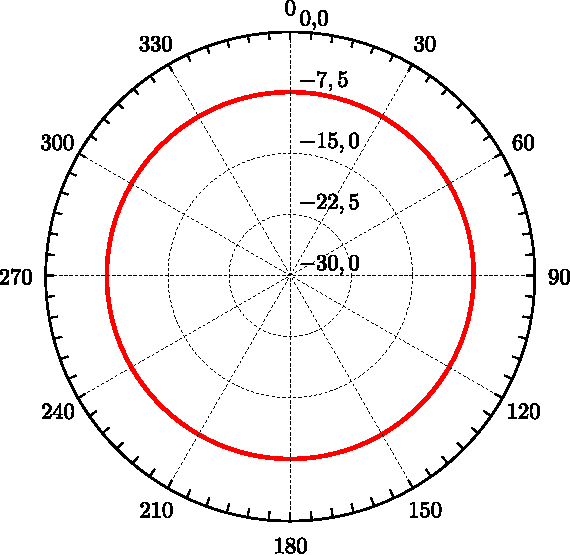
\includegraphics[scale = 1]{Figures/Estudio/estudio_1}
\caption{Diagrama de radiación del alimentador en el ángulo $\theta_0$.}
\label{fig_estudio:1}
\end{figure}
%%%%
A fin de determinar el alimentador requerido, se estudiaron las características de radiación de las siguientes antenas de abertura:
%%%%
\begin{itemize}
\item Abertura rectangular con plano conductor perfecto de extensión infinita y excitación con campo uniforme.
\item Abertura rectangular con plano conductor perfecto de extensión infinita y excitación con campo sinusoidal en modo dominante.
\item Abertura circular con plano conductor perfecto de extensión infinita y excitación con campo uniforme.
\item Abertura circular con plano conductor perfecto de extensión infinita y excitación con campo sinusoidal en modo dominante.
\item Guía de onda rectangular con extremo abierto.
\item Guía de onda cilíndrica con extremo abierto.
\item Bocina sectorial E.
\item Bocina sectorial H.
\item Bocina piramidal.
\item Bocina cónica.
\end{itemize}
%%%%
Para determinar las características de radiación de las antenas de abertura mencionadas anteriormente, se emplearon softwares de cálculo numérico (Matlab/Octave), a partir de las expresiones deducidas en los apéndices \ref{apendice_b} y \ref{apendice_c}. Para el caso de las antenas que sean excitadas con campo sinusoidal, se utilizan los modos dominantes, que corresponden al TE$_{10}$ para geometrías rectangulares y al TE$_{11}$ para geometrías circulares, cuyas expresiones han sido deducidas en el apéndice \ref{apendice_a}.

%%%%
\section{Aberturas con plano conductor perfecto de extensión infinita}
\label{sec_estudio_abert}
%%%%

Estas antenas son solamente modelos teóricos que se estudian con un fin didáctico previo al estudio de las antenas de abertura que son factibles de implementar en la práctica. La existencia de un plano conductor perfecto de extensión infinita concentra la radiación en valores de $\uptheta$ comprendidos entre 0$^{\circ}$ y 90$^{\circ}$.

%%%%
\subsection{Abertura rectangular con plano conductor perfecto de extensión infinita y excitación con campo uniforme}
\label{subsec_estudio_abert_rect_inf_uni}
%%%%

En la figura \ref{fig_estudio:2} se observa la geometría y las dimensiones de la abertura, y en las figuras \ref{fig_estudio:3} y \ref{grup_fig_estudio:1} se representan gráficamente los diagramas de radiación de la abertura con diferentes dimensiones, que se pueden observar en la tabla \ref{tabla_estudio:1}.
%%%%
\begin{figure}[H]
\centering
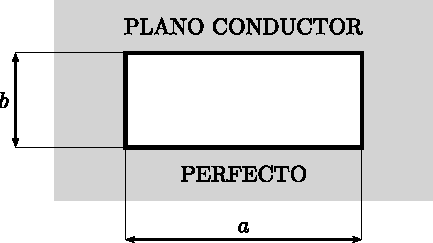
\includegraphics[scale = 1]{Figures/Estudio/estudio_2}
\caption{Dimensiones de la abertura rectangular con plano conductor perfecto de extensión infinita.}
\label{fig_estudio:2}
\end{figure}
%%%%
%%%%
\begin{figure}[H]
\centering
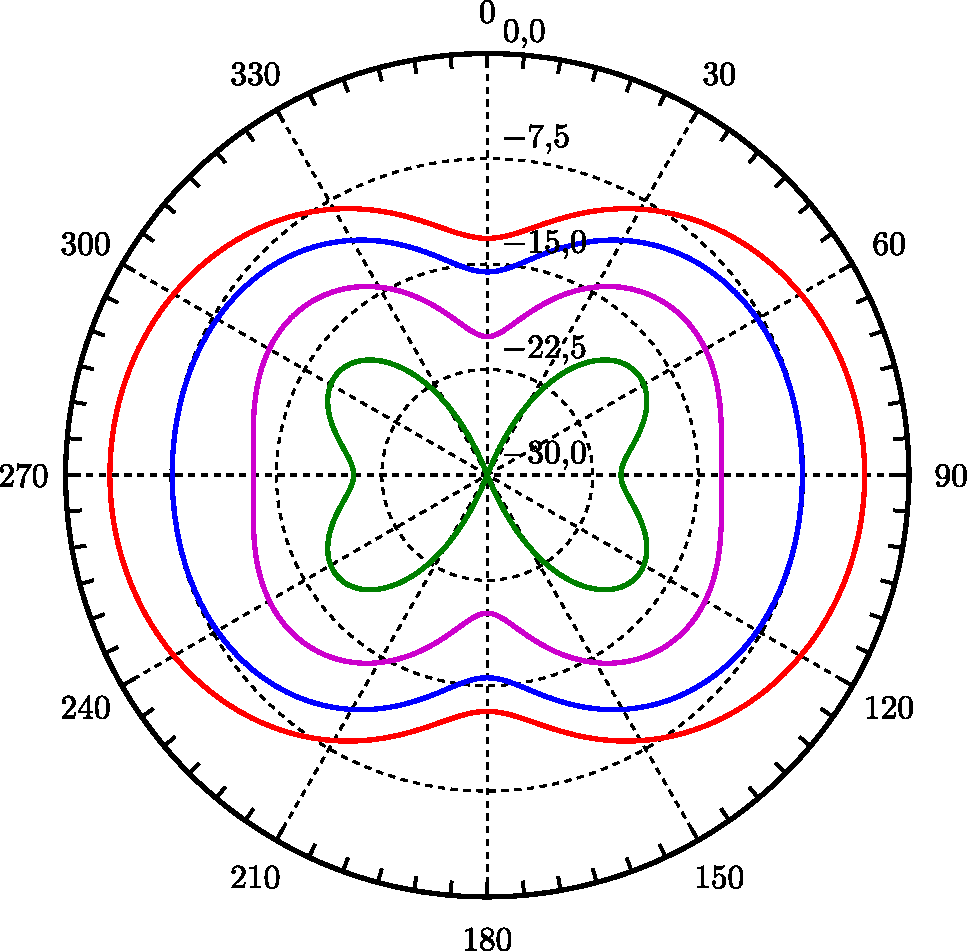
\includegraphics[scale = 0.5]{Figures/Estudio/estudio_3}
\caption{Diagramas de radiación en el ángulo $\theta_0$ de la abertura rectangular con plano conductor perfecto de extensión infinita y excitación con campo uniforme.}
\label{fig_estudio:3}
\end{figure}
%%%%
%%%%
\begin{figure} [H]
\centering 
\subfigure[Plano E.]{
\label{fig_estudio:4}
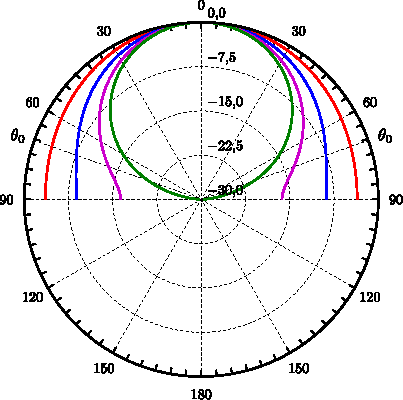
\includegraphics[scale = 1]{Figures/Estudio/estudio_4}}
\hspace{5mm}
\subfigure[Plano H.]{
\label{fig_estudio:5}
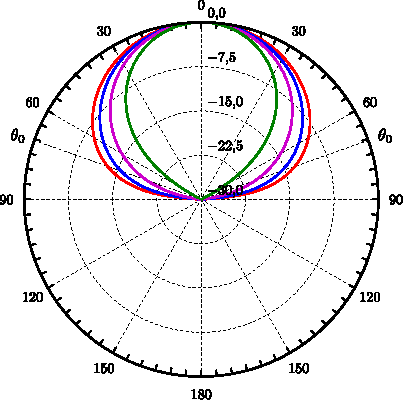
\includegraphics[scale = 1]{Figures/Estudio/estudio_5}}
\caption{Planos E y H de los diagramas de radiación de la abertura rectangular con plano conductor perfecto de extensión infinita y excitación con campo uniforme.}
\label{grup_fig_estudio:1}
\end{figure}
%%%%
\begin{table}[H]
\centering
\begin{tabular}{|c|c|c|c|c|c|}
\hline
\multirow{2}{*}{Trazo} & $a$ & $b$ & \multicolumn{2}{c|}{$G_{fn}\left(\theta_0\right)\,$(dB)} & $G_0$ \\
\cline{4-5}
& (mm) & (mm) & Plano E & Plano H & (dBi) \\
\hline

\includegraphics[scale = 1]{Figures/Estudio/linea_tabla_rojo} & 64,0 & 60,0 & -3,15 & -13,17 & 6,77 \\
\hline
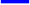
\includegraphics[scale = 1]{Figures/Estudio/linea_tabla_azul} & 80,0 & 88,0 & -7,59 & -15,56 & 8,51 \\
\hline
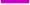
\includegraphics[scale = 1]{Figures/Estudio/linea_tabla_violeta} & 100,0 & 108,0 & -13,35 & -20,16 & 10,16 \\
\hline

\includegraphics[scale = 1]{Figures/Estudio/linea_tabla_verde} & 132,0 & 121,0 & -20,49 & -56,65 & 11,80 \\
\hline
\end{tabular}
\caption{Ganancia normalizada en el ángulo $\theta_0$ y ganancia máxima de la abertura rectangular con plano conductor perfecto de extensión infinita y excitación con campo uniforme.}
\label{tabla_estudio:1}
\end{table}
%%%%

%%%%
\subsection{Abertura rectangular con plano conductor perfecto de extensión infinita y excitación con campo sinusoidal en modo dominante}
\label{subsec_estudio_abert_rect_inf_dom}
%%%%

En la figura \ref{fig_estudio:2} se observa la geometría y las dimensiones de la abertura, y en las figuras \ref{fig_estudio:6} y \ref{grup_fig_estudio:2} se representan gráficamente los diagramas de radiación de la abertura con diferentes dimensiones, que se pueden observar en la tabla \ref{tabla_estudio:2}.
%%%%
\begin{figure}[H]
\centering
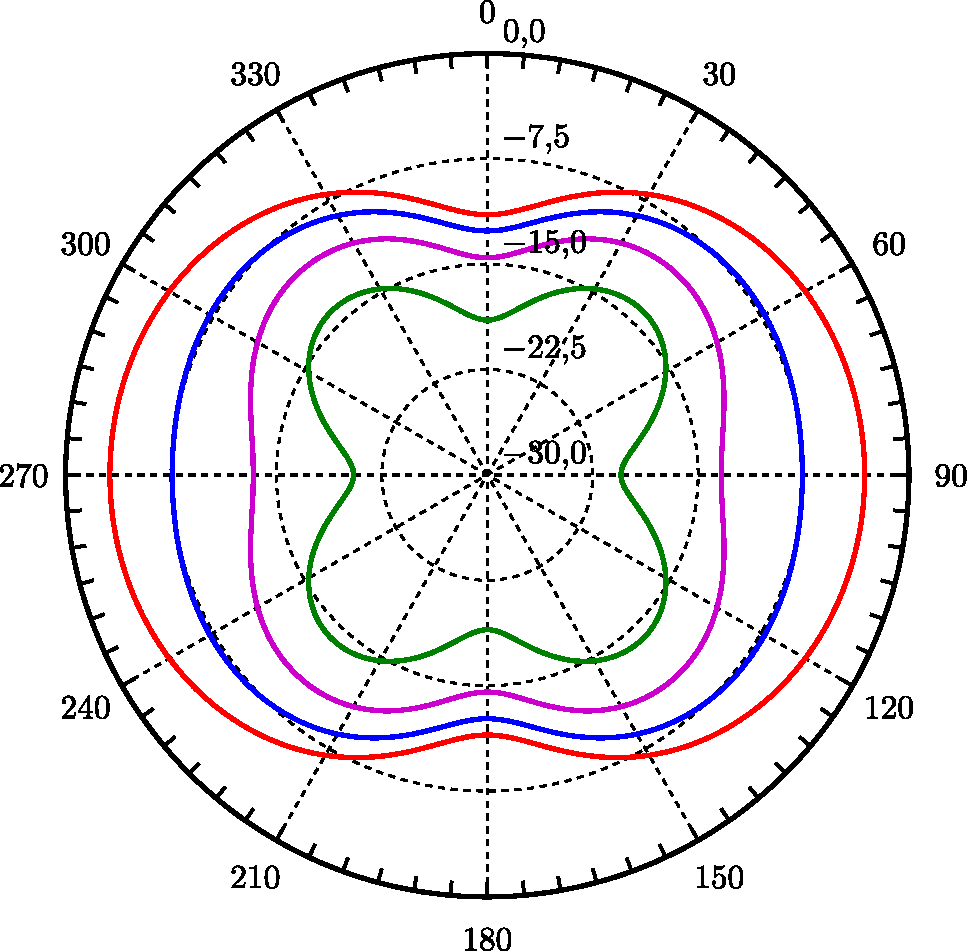
\includegraphics[scale = 0.5]{Figures/Estudio/estudio_6}
\caption{Diagramas de radiación en el ángulo $\theta_0$ de la abertura rectangular con plano conductor perfecto de extensión infinita y excitación con campo sinusoidal en modo dominante.}
\label{fig_estudio:6}
\end{figure}
%%%%
%%%%
\begin{figure} [H]
\centering 
\subfigure[Plano E.]{
\label{fig_estudio:7}
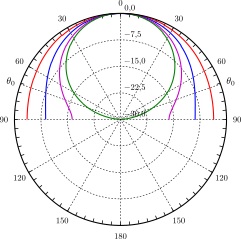
\includegraphics[scale = 1]{Figures/Estudio/estudio_7}}
\hspace{5mm}
\subfigure[Plano H.]{
\label{fig_estudio:8}
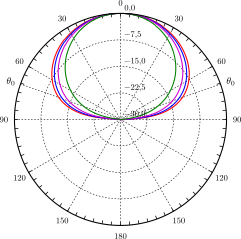
\includegraphics[scale = 1]{Figures/Estudio/estudio_8}}
\caption{Planos E y H de los diagramas de radiación de la abertura rectangular con plano conductor perfecto de extensión infinita y excitación con campo sinusoidal en modo dominante.}
\label{grup_fig_estudio:2}
\end{figure}
%%%%
\begin{table}[H]
\centering
\begin{tabular}{|c|c|c|c|c|c|}
\hline
\multirow{2}{*}{Trazo} & $a$ & $b$ & \multicolumn{2}{c|}{$G_{fn}\left(\theta_0\right)\,$(dB)} & $G_0$ \\
\cline{4-5}
& (mm) & (mm) & Plano E & Plano H & (dBi) \\
\hline

\includegraphics[scale = 1]{Figures/Estudio/linea_tabla_rojo} & 64,0 & 60,0 & -3,15 & -11,49 & 6,45 \\
\hline
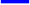
\includegraphics[scale = 1]{Figures/Estudio/linea_tabla_azul} & 80,0 & 88,0 & -7,59 & -12,65 & 8,00 \\
\hline
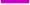
\includegraphics[scale = 1]{Figures/Estudio/linea_tabla_violeta} & 100,0 & 108,0 & -13,35 & -14,55 & 9,40 \\
\hline

\includegraphics[scale = 1]{Figures/Estudio/linea_tabla_verde} & 132,0 & 121,0 & -20,49 & -18,98 & 10,73 \\
\hline
\end{tabular}
\caption{Ganancia normalizada en el ángulo $\theta_0$ y ganancia máxima de la abertura rectangular con plano conductor perfecto de extensión infinita y excitación con campo sinusoidal en modo dominante.}
\label{tabla_estudio:2}
\end{table}
%%%%

%%%%
\subsection{Abertura circular con plano conductor perfecto de extensión infinita y excitación con campo uniforme}
\label{subsec_estudio_abert_circ_inf_uni}
%%%%

En la figura \ref{fig_estudio:9} se observa la geometría y las dimensiones de la abertura, y en las figuras \ref{fig_estudio:10} y \ref{grup_fig_estudio:3} se representan gráficamente los diagramas de radiación de la abertura con diferentes dimensiones, que se pueden observar en la tabla \ref{tabla_estudio:3}.
%%%%
\begin{figure}[H]
\centering
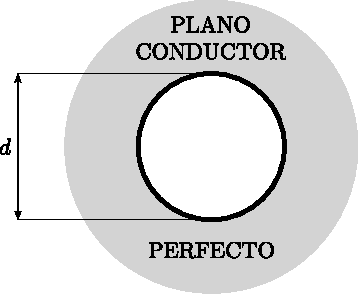
\includegraphics[scale = 1]{Figures/Estudio/estudio_9}
\caption{Dimensiones de la abertura circular con plano conductor perfecto de extensión infinita.}
\label{fig_estudio:9}
\end{figure}
%%%%
%%%%
\begin{figure}[H]
\centering
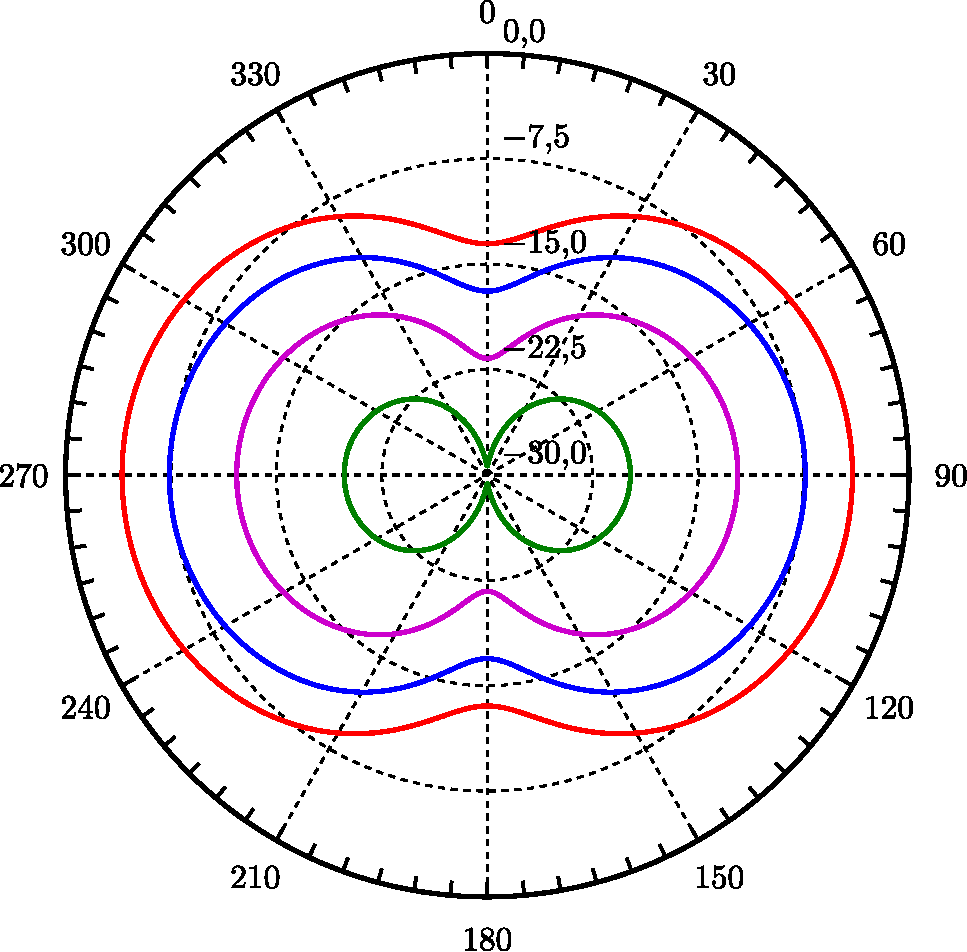
\includegraphics[scale = 0.5]{Figures/Estudio/estudio_10}
\caption{Diagramas de radiación en el ángulo $\theta_0$ de la abertura circular con plano conductor perfecto de extensión infinita y excitación con campo uniforme.}
\label{fig_estudio:10}
\end{figure}
%%%%
%%%%
\begin{figure} [H]
\centering 
\subfigure[Plano E.]{
\label{fig_estudio:11}
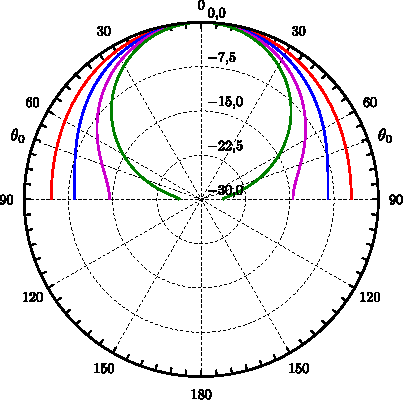
\includegraphics[scale = 1]{Figures/Estudio/estudio_11}}
\hspace{5mm}
\subfigure[Plano H.]{
\label{fig_estudio:12}
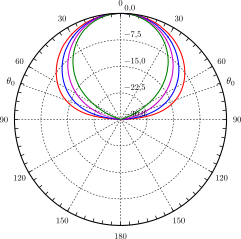
\includegraphics[scale = 1]{Figures/Estudio/estudio_12}}
\caption{Planos E y H de los diagramas de radiación de la abertura circular con plano conductor perfecto de extensión infinita y excitación con campo uniforme.}
\label{grup_fig_estudio:3}
\end{figure}
%%%%
\begin{table}[H]
\centering
\begin{tabular}{|c|c|c|c|c|}
\hline
\multirow{2}{*}{Trazo} & $d$ & \multicolumn{2}{c|}{$G_{fn}\left(\theta_0\right)\,$(dB)} & $G_0$ \\
\cline{3-4}
& (mm) & Plano E & Plano H & (dBi)\\
\hline

\includegraphics[scale = 1]{Figures/Estudio/linea_tabla_rojo} & 78,0 & -4,02 & -13,56 & 7,19 \\
\hline
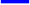
\includegraphics[scale = 1]{Figures/Estudio/linea_tabla_azul} & 102,0 & -7,38 & -16,93 & 8,80 \\
\hline
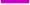
\includegraphics[scale = 1]{Figures/Estudio/linea_tabla_violeta} & 124,0 & -12,17 & -21,72 & 10,43 \\
\hline

\includegraphics[scale = 1]{Figures/Estudio/linea_tabla_verde} & 144,0 & -19,82 & -29,36 & 11,84 \\
\hline
\end{tabular}
\caption{Ganancia normalizada en el ángulo $\theta_0$ y ganancia máxima de la abertura circular con plano conductor perfecto de extensión infinita y excitación con campo uniforme.}
\label{tabla_estudio:3}
\end{table}
%%%%

%%%%
\subsection{Abertura circular con plano conductor perfecto de extensión infinita y excitación con campo sinusoidal en modo dominante}
\label{subsec_estudio_abert_circ_inf_dom}
%%%%

En la figura \ref{fig_estudio:9} se observa la geometría y las dimensiones de la abertura, y en las figuras \ref{fig_estudio:13} y \ref{grup_fig_estudio:4} se representan gráficamente los diagramas de radiación de la abertura con diferentes dimensiones, que se pueden observar en la tabla \ref{tabla_estudio:4}.
%%%%
\begin{figure}[H]
\centering
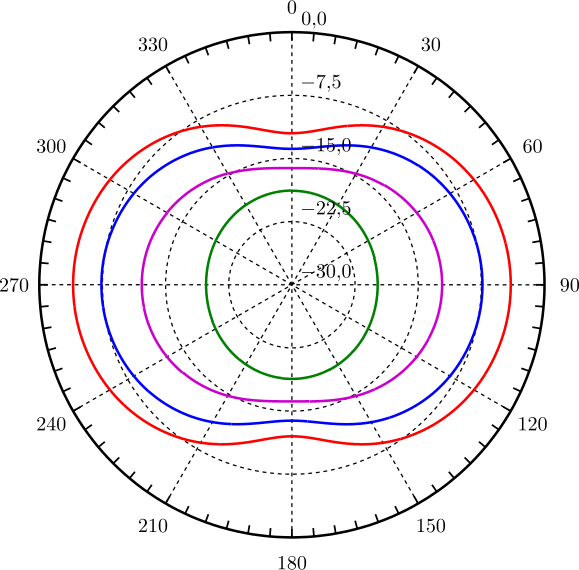
\includegraphics[scale = 0.5]{Figures/Estudio/estudio_13}
\caption{Diagramas de radiación en el ángulo $\theta_0$ de la abertura circular con plano conductor perfecto de extensión infinita y excitación con campo sinusoidal en modo dominante.}
\label{fig_estudio:13}
\end{figure}
%%%%
%%%%
\begin{figure} [H]
\centering 
\subfigure[Plano E.]{
\label{fig_estudio:14}
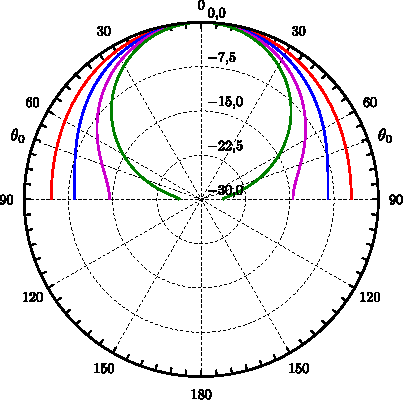
\includegraphics[scale = 1]{Figures/Estudio/estudio_14}}
\hspace{5mm}
\subfigure[Plano H.]{
\label{fig_estudio:15}
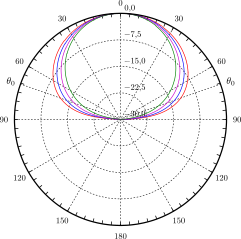
\includegraphics[scale = 1]{Figures/Estudio/estudio_15}}
\caption{Planos E y H de los diagramas de radiación de la abertura circular con plano conductor perfecto de extensión infinita y excitación con campo sinusoidal en modo dominante.}
\label{grup_fig_estudio:4}
\end{figure}
%%%%
\begin{table}[H]
\centering
\begin{tabular}{|c|c|c|c|c|}
\hline
\multirow{2}{*}{Trazo} & $d$ & \multicolumn{2}{c|}{$G_{fn}\left(\theta_0\right)\,$(dB)} & $G_0$ \\
\cline{3-4}
& (mm) & Plano E & Plano H & (dBi)\\
\hline

\includegraphics[scale = 1]{Figures/Estudio/linea_tabla_rojo} & 78,0 & -4,02 & -12,00 & 7,01 \\
\hline
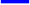
\includegraphics[scale = 1]{Figures/Estudio/linea_tabla_azul} & 102,0 & -7,38 & -13,86 & 8,46 \\
\hline
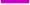
\includegraphics[scale = 1]{Figures/Estudio/linea_tabla_violeta} & 124,0 & -12,17 & -16,15 & 9,89 \\
\hline

\includegraphics[scale = 1]{Figures/Estudio/linea_tabla_verde} & 144,0 & -19,82 & -18,84 & 11,12 \\
\hline
\end{tabular}
\caption{Ganancia normalizada en el ángulo $\theta_0$ y ganancia máxima de la abertura circular con plano conductor perfecto de extensión infinita y excitación con campo sinusoidal en modo dominante.}
\label{tabla_estudio:4}
\end{table}
%%%%

%%%%
\section{Guías de onda con extremo abierto}
\label{sec_estudio_guias}
%%%%

Estas antenas pueden dimensionarse para que se propague solamente el modo dominante y su centro de fase se ubica en el centro de la abertura, generando así, luego de la reflexión en la superficie metálica del paraboloide, una fase constante a través del plano de abertura. Las dimensiones de las guías de onda pueden incrementarse, en caso de ser necesario, siempre y cuando no se propaguen modos de orden superior que afecten el funcionamiento de la antena.

%%%%
\subsection{Guía de onda rectangular con extremo abierto}
\label{subsec_estudio_guia_rect}
%%%%

En la figura \ref{fig_estudio:16} se observa la geometría y las dimensiones de la guía de onda, y en las figuras \ref{fig_estudio:17} y \ref{grup_fig_estudio:5} se representan gráficamente los diagramas de radiación de la guía de onda con diferentes dimensiones, que se pueden observar en la tabla \ref{tabla_estudio:5}.
%%%%
\begin{figure}[H]
\centering
\includegraphics[scale = 1]{Figures/Estudio/estudio_16}
\caption{Dimensiones de la guía de onda rectangular con extremo abierto.}
\label{fig_estudio:16}
\end{figure}
%%%%
%%%%
\begin{figure}[H]
\centering
\includegraphics[scale = 0.5]{Figures/Estudio/estudio_17}
\caption{Diagramas de radiación en el ángulo $\theta_0$ de la guía de onda rectangular con extremo abierto.}
\label{fig_estudio:17}
\end{figure}
%%%%
%%%%
\begin{figure} [H]
\centering 
\subfigure[Plano E.]{
\label{fig_estudio:18}
\includegraphics[scale = 1]{Figures/Estudio/estudio_18}}
\hspace{5mm}
\subfigure[Plano H.]{
\label{fig_estudio:19}
\includegraphics[scale = 1]{Figures/Estudio/estudio_19}}
\caption{Planos E y H de los diagramas de radiación de la guía de onda rectangular con extremo abierto.}
\label{grup_fig_estudio:5}
\end{figure}
%%%%
\begin{table}[H]
\centering
\begin{tabular}{|c|c|c|c|c|c|}
\hline
\multirow{2}{*}{Trazo} & $a$ & $b$ & \multicolumn{2}{c|}{$G_{fn}\left(\theta_0\right)\,$(dB)} & $G_0$ \\
\cline{4-5}
& (mm) & (mm) & Plano E & Plano H & (dBi)\\
\hline
\includegraphics[scale = 1]{Figures/Estudio/linea_tabla_rojo} & 64,0 & 30,0 & -4,27 & -5,47 & 5,64 \\
\hline
\includegraphics[scale = 1]{Figures/Estudio/linea_tabla_azul} & 90,0 & 67,0 & -7,54 & -7,51 & 7,17 \\
\hline
\includegraphics[scale = 1]{Figures/Estudio/linea_tabla_violeta} & 130,0 & 90,0 & -11,55 & -12,62 & 9,16 \\
\hline
\includegraphics[scale = 1]{Figures/Estudio/linea_tabla_verde} & 152,0 & 121,0 & -24,01 & -17,06 & 11,09 \\
\hline
\end{tabular}
\caption{Ganancia normalizada en el ángulo $\theta_0$ y ganancia máxima de la guía de onda rectangular con extremo abierto.}
\label{tabla_estudio:5}
\end{table}
%%%%

%%%%
\subsection{Guía de onda cilíndrica con extremo abierto}
\label{subsec_estudio_guia_cili}
%%%%

En la figura \ref{fig_estudio:20} se observa la geometría y las dimensiones de la guía de onda, y en las figuras \ref{fig_estudio:21} y \ref{grup_fig_estudio:6} se representan gráficamente los diagramas de radiación de la guía de onda con diferentes dimensiones, que se pueden observar en la tabla \ref{tabla_estudio:6}.
%%%%
\begin{figure}[H]
\centering
\includegraphics[scale = 1]{Figures/Estudio/estudio_20}
\caption{Dimensiones de la guía de onda cilíndrica con extremo abierto.}
\label{fig_estudio:20}
\end{figure}
%%%%
%%%%
\begin{figure}[H]
\centering
\includegraphics[scale = 0.5]{Figures/Estudio/estudio_21}
\caption{Diagramas de radiación en el ángulo $\theta_0$ de la guía de onda cilíndrica con extremo abierto.}
\label{fig_estudio:21}
\end{figure}
%%%%
%%%%
\begin{figure} [H]
\centering 
\subfigure[Plano E.]{
\label{fig_estudio:22}
\includegraphics[scale = 1]{Figures/Estudio/estudio_22}}
\hspace{5mm}
\subfigure[Plano H.]{
\label{fig_estudio:23}
\includegraphics[scale = 1]{Figures/Estudio/estudio_23}}
\caption{Planos E y H de los diagramas de radiación de la guía de onda cilíndrica con extremo abierto.}
\label{grup_fig_estudio:6}
\end{figure}
%%%%
\begin{table}[H]
\centering
\begin{tabular}{|c|c|c|c|c|}
\hline
\multirow{2}{*}{Trazo} & $d$ & \multicolumn{2}{c|}{$G_{fn}\left(\theta_0\right)\,$(dB)} & $G_0$ \\
\cline{3-4}
& (mm) & Plano E & Plano H & (dBi)\\
\hline
\includegraphics[scale = 1]{Figures/Estudio/linea_tabla_rojo} & 86,0 & -8,51 & -6,53 & 7,15 \\
\hline
\includegraphics[scale = 1]{Figures/Estudio/linea_tabla_azul} & 108,0 & -12,00 & -8,40 & 8,39 \\
\hline
\includegraphics[scale = 1]{Figures/Estudio/linea_tabla_violeta} & 130,0 & -17,49 & -10,87 & 9,74 \\
\hline
\includegraphics[scale = 1]{Figures/Estudio/linea_tabla_verde} & 152,0 & -29,10 & -14,10 & 11,06 \\
\hline
\end{tabular}
\caption{Ganancia normalizada en el ángulo $\theta_0$ y ganancia máxima de la guía de onda cilíndrica con extremo abierto.}
\label{tabla_estudio:6}
\end{table}
%%%%

%%%%
\section{Bocinas}
\label{sec_estudio_bocinas}
%%%%

Las bocinas están compuestas básicamente por una guía de onda cuya sección se va incrementando paulatinamente hasta un extremo abierto, que se comporta como abertura. La guía de onda se dimensiona de forma tal que se propague solamente el modo dominante, y variando las dimensiones de la abertura es posible obtener la ganancia deseada sin que se propaguen otros modos, lo que constituye una clara ventaja respecto a las guías de onda con extremo abierto. No obstante, debido a que en la transición entre el extremo abierto de la guía de onda y la abertura se va incrementando la sección, el centro de fase no se ubicará en centro de la abertura, por lo que la fase a través del plano de abertura de las ondas radiadas, luego de reflejarse en el paraboloide, no será constante.

%%%%
\subsection{Bocina sectorial E}
\label{subsec_estudio_boci_sece}
%%%%

En las figuras \ref{fig_estudio:24} y \ref{fig_estudio:25} se observa la geometría y las dimensiones de la bocina, y en las figuras \ref{fig_estudio:26} y \ref{grup_fig_estudio:7} se representan gráficamente los diagramas de radiación de la bocina con diferentes dimensiones, que se pueden observar en la tabla \ref{tabla_estudio:7}.
%%%%
\begin{figure}[H]
\centering
\includegraphics[scale = 1]{Figures/Estudio/estudio_24}
\caption{Dimensiones de la bocina sectorial E.}
\label{fig_estudio:24}
\end{figure}
%%%%
%%%%
\begin{figure}[H]
\centering
\includegraphics[scale = 1]{Figures/Estudio/estudio_25}
\caption{Corte en el plano E de la bocina sectorial E.}
\label{fig_estudio:25}
\end{figure}
%%%%
%%%%
\begin{figure}[H]
\centering
\includegraphics[scale = 0.5]{Figures/Estudio/estudio_26}
\caption{Diagramas de radiación en el ángulo $\theta_0$ de la bocina sectorial E.}
\label{fig_estudio:26}
\end{figure}
%%%%
%%%%
\begin{figure} [H]
\centering 
\subfigure[Plano E.]{
\label{fig_estudio:27}
\includegraphics[scale = 1]{Figures/Estudio/estudio_27}}
\hspace{5mm}
\subfigure[Plano H.]{
\label{fig_estudio:28}
\includegraphics[scale = 1]{Figures/Estudio/estudio_28}}
\caption{Planos E y H de los diagramas de radiación de la bocina sectorial E.}
\label{grup_fig_estudio:7}
\end{figure}
%%%%
\begin{table}[H]
\centering
\begin{tabular}{|c|c|c|c|c|c|c|c|}
\hline
\multirow{2}{*}{Trazo} & $a$ & $b$ & $B$ & $L$ & \multicolumn{2}{c|}{$G_{fn}\left(\theta_0\right)\,$(dB)} & $G_0$ \\
\cline{6-7}
& (mm) & (mm) & (mm) & (mm) & Plano E & Plano H & (dBi)\\
\hline
\includegraphics[scale = 1]{Figures/Estudio/linea_tabla_rojo} & 90,0 & 43,0 & 67,0 & 100,0 & -7,54 & -7,51 & 7,17 \\
\hline
\includegraphics[scale = 1]{Figures/Estudio/linea_tabla_azul} & 99,0 & 43,0 & 100,0 & 100,0 & -13,93 & -8,42 & 8,64 \\
\hline
\includegraphics[scale = 1]{Figures/Estudio/linea_tabla_violeta} & 109,0 & 55,0 & 120,0 & 120,0 & -21,17 & -9,58 & 9,69 \\
\hline
\includegraphics[scale = 1]{Figures/Estudio/linea_tabla_verde} & 119,0 & 55,0 & 150,0 & 150,0 & -19,32 & -10,92 & 10,91 \\
\hline
\end{tabular}
\caption{Ganancia normalizada en el ángulo $\theta_0$ y ganancia máxima de la bocina sectorial E.}
\label{tabla_estudio:7}
\end{table}
%%%%

%%%%
\subsection{Bocina sectorial H}
\label{subsec_estudio_boci_sech}
%%%%

En las figuras \ref{fig_estudio:29} y \ref{fig_estudio:30} se observa la geometría y las dimensiones de la bocina, y en las figuras \ref{fig_estudio:31} y \ref{grup_fig_estudio:8} se representan gráficamente los diagramas de radiación de la bocina con diferentes dimensiones, que se pueden observar en la tabla \ref{tabla_estudio:8}.
%%%%
\begin{figure}[H]
\centering
\includegraphics[scale = 1]{Figures/Estudio/estudio_29}
\caption{Dimensiones de la bocina sectorial H.}
\label{fig_estudio:29}
\end{figure}
%%%%
%%%%
\begin{figure}[H]
\centering
\includegraphics[scale = 1]{Figures/Estudio/estudio_30}
\caption{Corte en el plano H de la bocina sectorial H.}
\label{fig_estudio:30}
\end{figure}
%%%%
%%%%
\begin{figure}[H]
\centering
\includegraphics[scale = 0.5]{Figures/Estudio/estudio_31}
\caption{Diagramas de radiación en el ángulo $\theta_0$ de la bocina sectorial H.}
\label{fig_estudio:31}
\end{figure}
%%%%
%%%%
\begin{figure} [H]
\centering 
\subfigure[Plano E.]{
\label{fig_estudio:32}
\includegraphics[scale = 1]{Figures/Estudio/estudio_32}}
\hspace{5mm}
\subfigure[Plano H.]{
\label{fig_estudio:33}
\includegraphics[scale = 1]{Figures/Estudio/estudio_33}}
\caption{Planos E y H de los diagramas de radiación de la bocina sectorial H.}
\label{grup_fig_estudio:8}
\end{figure}
%%%%
\begin{table}[H]
\centering
\begin{tabular}{|c|c|c|c|c|c|c|c|}
\hline
\multirow{2}{*}{Trazo} & $a$ & $b$ & $A$ & $L$ & \multicolumn{2}{c|}{$G_{fn}\left(\theta_0\right)\,$(dB)} & $G_0$ \\
\cline{6-7}
& (mm) & (mm) & (mm) & (mm) & Plano E & Plano H & (dBi)\\
\hline
\includegraphics[scale = 1]{Figures/Estudio/linea_tabla_rojo} & 75,0 & 67,0 & 90,0 & 100,0 & -7,54 & -7,51 & 7,17 \\
\hline
\includegraphics[scale = 1]{Figures/Estudio/linea_tabla_azul} & 75,0 & 77,0 & 120,0 & 100,0 & -9,03 & -11,00 & 8,34 \\
\hline
\includegraphics[scale = 1]{Figures/Estudio/linea_tabla_violeta} & 109,0 & 87,0 & 150,0 & 120,0 & -10,90 & -16,38 & 9,61 \\
\hline
\includegraphics[scale = 1]{Figures/Estudio/linea_tabla_verde} & 109,0 & 97,0 & 200,0 & 150,0 & -13,29 & -24,46 & 11,23 \\
\hline
\end{tabular}
\caption{Ganancia normalizada en el ángulo $\theta_0$ y ganancia máxima de la bocina sectorial H.}
\label{tabla_estudio:8}
\end{table}
%%%%

%%%%
\subsection{Bocina piramidal}
\label{subsec_estudio_boci_pira}
%%%%

En las figuras \ref{fig_estudio:34}, \ref{fig_estudio:35} y \ref{fig_estudio:36} se observa la geometría y las dimensiones de la bocina, y en las figuras \ref{fig_estudio:37} y \ref{grup_fig_estudio:9} se representan gráficamente los diagramas de radiación de la bocina con diferentes dimensiones, que se pueden observar en la tabla \ref{tabla_estudio:9}.
%%%%
\begin{figure}[H]
\centering
\includegraphics[scale = 1]{Figures/Estudio/estudio_34}
\caption{Dimensiones de la bocina piramidal.}
\label{fig_estudio:34}
\end{figure}
%%%%
%%%%
\begin{figure}[H]
\centering
\includegraphics[scale = 1]{Figures/Estudio/estudio_35}
\caption{Corte en el plano E de la bocina piramidal.}
\label{fig_estudio:35}
\end{figure}
%%%%
%%%%
\begin{figure}[H]
\centering
\includegraphics[scale = 1]{Figures/Estudio/estudio_36}
\caption{Corte en el plano H de la bocina piramidal.}
\label{fig_estudio:36}
\end{figure}
%%%%
%%%%
\begin{figure}[H]
\centering
\includegraphics[scale = 0.5]{Figures/Estudio/estudio_37}
\caption{Diagramas de radiación en el ángulo $\theta_0$ de la bocina piramidal.}
\label{fig_estudio:37}
\end{figure}
%%%%
%%%%
\begin{figure} [H]
\centering 
\subfigure[Plano E.]{
\label{fig_estudio:38}
\includegraphics[scale = 1]{Figures/Estudio/estudio_38}}
\hspace{5mm}
\subfigure[Plano H.]{
\label{fig_estudio:39}
\includegraphics[scale = 1]{Figures/Estudio/estudio_39}}
\caption{Planos E y H de los diagramas de radiación de la bocina piramidal.}
\label{grup_fig_estudio:9}
\end{figure}
%%%%
%%%%
\begin{table}[H]
\centering
\begin{tabular}{|c|c|c|c|c|c|c|c|c|}
\hline
\multirow{2}{*}{Trazo} & $a$ & $b$ & $A$ & $B$ & $L$ & \multicolumn{2}{c|}{$G_{fn}\left(\theta_0\right)\,$(dB)} & $G_0$ \\
\cline{7-8}
& (mm) & (mm) & (mm) & (mm) & (mm) & Plano E & Plano H & (dBi)\\
\hline
\includegraphics[scale = 1]{Figures/Estudio/linea_tabla_rojo} & 75,0 & 43,0 & 90,0 & 67,0 & 100,0 & -7,54 & -7,51 & 7,17 \\
\hline
\includegraphics[scale = 1]{Figures/Estudio/linea_tabla_azul} & 86,0 & 43,0 & 120,0 & 90,0 & 100,0 & -11,49 & -11,02 & 8,86 \\
\hline
\includegraphics[scale = 1]{Figures/Estudio/linea_tabla_violeta} & 97,0 & 55,0 & 150,0 & 110,0 & 120,0 & -17,29 & -16,26 & 10,56 \\
\hline
\includegraphics[scale = 1]{Figures/Estudio/linea_tabla_verde} & 108,0 & 55,0 & 200,0 & 150,0 & 150,0 & -19,32 & -24,37 & 13,09 \\
\hline
\end{tabular}
\caption{Ganancia normalizada en el ángulo $\theta_0$ y ganancia máxima de la bocina piramidal.}
\label{tabla_estudio:9}
\end{table}
%%%%

%%%%
\subsection{Bocina cónica}
\label{subsec_estudio_boci_coni}
%%%%

En las figuras \ref{fig_estudio:40} y \ref{fig_estudio:41} se observa la geometría y las dimensiones de la bocina, y en las figuras \ref{fig_estudio:42} y \ref{grup_fig_estudio:10} se representan gráficamente los diagramas de radiación de la bocina con diferentes dimensiones, que se pueden observar en la tabla \ref{tabla_estudio:10}.
%%%%
\begin{figure}[H]
\centering
\includegraphics[scale = 1]{Figures/Estudio/estudio_40}
\caption{Dimensiones de la bocina cónica.}
\label{fig_estudio:40}
\end{figure}
%%%%
%%%%
\begin{figure}[H]
\centering
\includegraphics[scale = 1]{Figures/Estudio/estudio_41}
\caption{Corte longitudinal de la bocina cónica.}
\label{fig_estudio:41}
\end{figure}
%%%%
%%%%
\begin{figure}[H]
\centering
\includegraphics[scale = 0.5]{Figures/Estudio/estudio_42}
\caption{Diagramas de radiación en el ángulo $\theta_0$ de la bocina cónica.}
\label{fig_estudio:42}
\end{figure}
%%%%
%%%%
\begin{figure} [H]
\centering 
\subfigure[Plano E.]{
\label{fig_estudio:43}
\includegraphics[scale = 1]{Figures/Estudio/estudio_43}}
\hspace{5mm}
\subfigure[Plano H.]{
\label{fig_estudio:44}
\includegraphics[scale = 1]{Figures/Estudio/estudio_44}}
\caption{Planos E y H de los diagramas de radiación de la bocina cónica.}
\label{grup_fig_estudio:10}
\end{figure}
%%%%
%%%%
\begin{table}[H]
\centering
\begin{tabular}{|c|c|c|c|c|c|c|}
\hline
\multirow{2}{*}{Trazo} & $d$ & $D$ & $L$ & \multicolumn{2}{c|}{$G_{fn}\left(\theta_0\right)\,$(dB)} & $G_0$ \\
\cline{5-6}
& (mm) & (mm) & (mm) & Plano E & Plano H & (dBi)\\
\hline
\includegraphics[scale = 1]{Figures/Estudio/linea_tabla_rojo} & 80,0 & 86,0 & 100,0 & -8,51 & -6,53 & 7,15 \\
\hline
\includegraphics[scale = 1]{Figures/Estudio/linea_tabla_azul} & 84,0 & 136,0 & 100,0 & -18,97 & -11,63 & 10,08 \\
\hline
\includegraphics[scale = 1]{Figures/Estudio/linea_tabla_violeta} & 98,0 & 180,0 & 120,0 & -21,50 & -19,34 & 12,39 \\
\hline
\includegraphics[scale = 1]{Figures/Estudio/linea_tabla_verde} & 98,0 & 220,0 & 150,0 & -18,98 & -25,72 & 13,84 \\
\hline
\end{tabular}
\caption{Ganancia normalizada en el ángulo $\theta_0$ y ganancia máxima de la bocina cónica.}
\label{tabla_estudio:10}
\end{table}
%%%%

%%%%
\section{Selección del alimentador}
\label{sec_selec_alim}
%%%%

Para el reflector parabólico a utilizar, la relación $F/D$, como se vió en la sección \ref{sec_estudio_param}, es de 0,353. Descartadas las aberturas con plano conductor perfecto de extensión infinita por tratarse de modelos teóricos, la elección recae necesariamente en una guía de onda con extremo abierto o en una bocina. Como se ha visto en los diagramas de radiación en la sección \ref{sec_estudio_bocinas}, es posible dimensionar los distintos tipos de bocinas para obtener la iluminación deseada, según la expresión \eqref{ec_estudio:3}. Sin embargo, tal dimensionamiento implica que la abertura debe tener dimensiones similares a la guía de onda empleada en las bocinas.

Las guías de onda con extremo abierto también generan la iluminación deseada. Considerando las dimensiones de las guías de onda que cumplen con la condición de iluminación obtenidas de las tablas \ref{tabla_estudio:5} y \ref{tabla_estudio:6}, en la tabla \ref{tabla_estudio:11} se muestran las frecuencias de corte tanto para el modo dominante como para el siguiente modo de propagación.
%%%%
\begin{table}[H]
\centering
\begin{tabular}{|c|c|c|c|c|c|}
\hline
\multirow{2}{*}{Guía de} & \multirow{2}{*}{Dimensiones} & \multirow{2}{*}{Modo} & \multirow{2}{*}{1.$^{\text{er}}$ modo} & \multicolumn{1}{c|}{f$_\text{c}$ modo} & \multicolumn{1}{c|}{f$_\text{c}$ 1.$^{\text{er}}$ modo} \\
\multirow{2}{*}{onda} & \multirow{2}{*}{(mm)} & \multirow{2}{*}{dominante} & \multirow{2}{*}{superior} & dominante & superior \\
& & & & (GHz) & (GHz) \\
\hline
\multirow{2}{*}{Rectangular} & \multicolumn{1}{c|}{ancho = 90,0} & \multirow{2}{*}{TE$_{10}$} & \multirow{2}{*}{TE$_{01}$} & \multirow{2}{*}{1,67} & \multirow{2}{*}{2,24} \\
& alto = 67,0 & & & & \\
\hline
Cilíndrica & diámetro = 86,0 & TE$_{11}$ & TM$_{01}$ & 2,04 & 2,67 \\
\hline
\end{tabular}
\caption{Frecuencias de corte para el modo dominante y para el siguiente modo de propagación de las guías de onda con extremo abierto (ver apéndice \ref{apendice_a}  y \cite{Balaniselectro}).}
\label{tabla_estudio:11}
\end{table}
%%%%
Puede observarse que a la frecuencia de operación, la guía de onda rectangular propaga, además del modo dominante TE$_{10}$, el modo TE$_{01}$, mientras que la guía de onda cilíndrica propaga solamente el modo dominante TE$_{11}$.

Para determinar la distribuciones de campos generadas por los alimentadores estudiados, se ha empleado un método numérico basándose en la óptica geométrica: conociendo las densidades de corriente equivalentes sobre la abertura, se las integra para obtener los campos radiados. Un aspecto a considerar es que, al emplear este método para determinar los campos radiados, se asume que los campos eléctrico y mágnético sobre la abertura están relacionados como en una onda transverso-electromagnética ($\mathbf{TEM}$) \cite{Balanisantenas}:
%%%%
\begin{align}
\mathbf{H}_a \simeq \versor{n}\prodvec\dfrac{\mathbf{E}_a}{\eta}
\label{ec_estudio:4}
\end{align}
%%%%
Esta aproximación es válida en la medida que las dimensiones de la abertura sean lo suficientemente grandes como para considerar que los campos $\mathbf{E}_a$ y $\mathbf{H}_a$ constituyen una onda plana; en otras palabras, la aproximación es válida para aberturas con una ganancia moderada o alta. Claramente dicha aproximación pierde validez para las dimensiones de las guías de onda con extremo abierto necesarias para cumplir los parámetros de iluminación.

Un factor muy importante que la óptica geométrica no considera es la difracción producida en los bordes de los alimentadores; este fenómeno podrá alterar la distribución espacial de campos.

Para determinar la precisión con la que el modelo matemático predice la distribución de los campos radiados por ambas guías de onda, se realizaron simulaciones con el software FEKO para poder comparar los resultados obtenidos mediante la simulación con el método numérico basado en la óptica geométrica implementado con el software MATLAB/OCTAVE.

En las figuras \ref{fig_estudio:45} y \ref{grup_fig_estudio:12} se comparan los diagramas de radiación de la guía de onda rectangular con extremo abierto correspondientes al modelo teórico y a la simulación, y en la tabla \ref{tabla_estudio:12} se compara $G_{fn}\left(\theta_0\right)$ en los planos E y H y la ganancia máxima $G_0$.
%%%%
\begin{figure}[H]
\centering
\includegraphics[scale = 0.5]{Figures/Estudio/estudio_45}
\caption{Diagramas de radiación en el ángulo $\theta_0$ de la guía de onda rectangular con extremo abierto (modelo teórico y simulación).}
\label{fig_estudio:45}
\end{figure}
%%%%
%%%%
\begin{figure} [H]
\centering 
\subfigure[Plano E.]{
\label{fig_estudio:46}
\includegraphics[scale = 1]{Figures/Estudio/estudio_46}}
\hspace{5mm}
\subfigure[Plano H.]{
\label{fig_estudio:47}
\includegraphics[scale = 1]{Figures/Estudio/estudio_47}}
\caption{Planos E y H de los diagramas de radiación de la guía de onda rectangular con extremo abierto (modelo teórico y simulación).}
\label{grup_fig_estudio:12}
\end{figure}
%%%%
%%%%
\begin{table}[H]
\centering
\begin{tabular}{|c|c|c|c|c|c|c|}
\hline
\multirow{2}{*}{Método} & \multirow{2}{*}{Trazo} & $a$ & $b$ & \multicolumn{2}{c|}{$G_{fn}\left(\theta_0\right)\,$(dB)} & $G_0$ \\
\cline{5-6}
& & (mm) & (mm) & Plano E & Plano H & (dBi)\\
\hline
Modelo teórico & \includegraphics[scale = 1]{Figures/Estudio/linea_tabla_rojo} & 90,0 & 67,0 & -7,54 & -7,51 & 7,17 \\
\hline
Simulación & \includegraphics[scale = 1]{Figures/Estudio/linea_tabla_azul} & 90,0 & 67,0 & -6,66 & -12,46 & 7,72 \\
\hline
\end{tabular}
\caption{Ganancia normalizada en el ángulo $\theta_0$ y ganancia máxima de la guía de onda rectangular con extremo abierto (modelo teórico y simulación).}
\label{tabla_estudio:12}
\end{table}
%%%%
En las figuras \ref{fig_estudio:48} y \ref{grup_fig_estudio:13} se comparan los diagramas de radiación de la guía de onda cilíndrica con extremo abierto correspondientes al modelo teórico y a la simulación, y en la tabla \ref{tabla_estudio:13} se compara $G_{fn}\left(\theta_0\right)$ en los planos E y H y la ganancia máxima $G_0$.
%%%%
\begin{figure}[H]
\centering
\includegraphics[scale = 0.5]{Figures/Estudio/estudio_48}
\caption{Diagramas de radiación en el ángulo $\theta_0$ de la guía de onda cilíndrica con extremo abierto (modelo teórico y simulación).}
\label{fig_estudio:48}
\end{figure}
%%%%
%%%%
\begin{figure} [H]
\centering 
\subfigure[Plano E.]{
\label{fig_estudio:49}
\includegraphics[scale = 1]{Figures/Estudio/estudio_49}}
\hspace{5mm}
\subfigure[Plano H.]{
\label{fig_estudio:50}
\includegraphics[scale = 1]{Figures/Estudio/estudio_50}}
\caption{Planos E y H de los diagramas de radiación de la guía de onda cilíndrica con extremo abierto (modelo teórico y simulación).}
\label{grup_fig_estudio:13}
\end{figure}
%%%%
%%%%
\begin{table}[H]
\centering
\begin{tabular}{|c|c|c|c|c|c|}
\hline
\multirow{2}{*}{Método} & \multirow{2}{*}{Trazo} & $d$ & \multicolumn{2}{c|}{$G_{fn}\left(\theta_0\right)\,$(dB)} & $G_0$ \\
\cline{4-5}
& & (mm) & Plano E & Plano H & (dBi)\\
\hline
Modelo teórico & \includegraphics[scale = 1]{Figures/Estudio/linea_tabla_rojo} & 86,0 & -8,51 & -6,53 & 7,15 \\
\hline
Simulación & \includegraphics[scale = 1]{Figures/Estudio/linea_tabla_azul} & 86,0 & -8,36 & -9,43 & 7,59 \\
\hline
\end{tabular}
\caption{Ganancia normalizada en el ángulo $\theta_0$ y ganancia máxima de la guía de onda cilíndrica con extremo abierto (modelo teórico y simulación).}
\label{tabla_estudio:13}
\end{table}
%%%%
A partir de la comparaciones realizadas, puede observarse que mediante el modelo teórico puede obtenerse una buena aproximación de la ganancia máxima, pero debido a la difracción producida en los bordes de la abertura la distribución de campos no puede aproximarse con un error relativamente bajo; dicho efecto se evidencia fundamentalmente en el Plano H del diagrama de radiación y en la aparición de un lóbulo posterior.

En los diagramas de radiación de las figuras \ref{fig_estudio:45} - \ref{grup_fig_estudio:13} se evidencia que la guía de onda cilíndrica es menos afectada por la difracción que la guía de onda rectangular; en otras palabras, la distribución de campos generada por la guía de onda cilíndrica es la que más se acerca a los parámetros de iluminación deseados. Además, la guía de onda cilíndrica no permite la propagación de modos de orden superior a la frecuencia de operación. Por lo tanto, se concluye que la guía cilíndrica con extremo abierto es la estructura que mejor se ajusta a los parámetros de iluminación deseados.

Empleando el software de simulación, se redimensiona la guía de onda cilíndrica con extremo abierto para obtener la iluminación deseada. Para un diámetro de 83 mm, los diagramas de radiación obtenidos son los que se observan en las figuras \ref{fig_estudio:51} y \ref{grup_fig_estudio:14}.
%%%%
\begin{figure}[H]
\centering
\includegraphics[scale = 0.5]{Figures/Estudio/estudio_51}
\caption{Diagrama de radiación en el ángulo $\theta_0$ de la guía de onda cilíndrica con extremo abierto simulada, para un diámetro de 83 mm.}
\label{fig_estudio:51}
\end{figure}
%%%%
%%%%
\begin{figure} [H]
\centering 
\subfigure[Plano E.]{
\label{fig_estudio:52}
\includegraphics[scale = 1]{Figures/Estudio/estudio_52}}
\hspace{5mm}
\subfigure[Plano H.]{
\label{fig_estudio:53}
\includegraphics[scale = 1]{Figures/Estudio/estudio_53}}
\caption{Planos E y H del diagrama de radiación de la guía de onda cilíndrica con extremo abierto simulada, para un diámetro de 83 mm.}
\label{grup_fig_estudio:14}
\end{figure}
%%%%
Observando la figura \ref{fig_estudio:51}, puede decirse que una guía de onda cilíndrica con extremo abierto con un diámetro de 83 mm se ajusta satisfactoriamente a los parámetros de iluminación deseados. Sin embargo, debido a la difracción en el borde de la abertura se genera un lóbulo de radiación posterior, que se evidencia claramente en las figuras \ref{grup_fig_estudio:14}.

Con el fin de atenuar el lóbulo posterior, se estudia un alimentador que consiste en una guía de onda cilíndrica con extremo abierto y que posee una estructura anular cerca de la abertura, la cual se comporta como un choque. En la figura \ref{fig_estudio:54} puede observarse un gráfico de esta antena.
%%%%
\begin{figure}[H]
\centering
\includegraphics[scale = 1]{Figures/Estudio/estudio_54}
\caption{Guía de onda cilíndrica con choque anular.}
\label{fig_estudio:54}
\end{figure}
%%%%
Este tipo de antena puede tener no solamente un choque, sino dos, tres o más, y además, la longitud de los choques y la separación entre los mismos no debe ser necesariamente la misma \cite{James}. Debido a que una de las características deseadas del alimentador es que sus dimensiones sean lo más reducidas posibles para maximizar la eficiencia por bloqueo $\varepsilon_b$, se considera el estudio de la antena con un solo choque. En la figura \ref{fig_estudio:55} puede observarse un corte longitudinal de una guía de onda cilíndrica con sólo un choque.
%%%%
\begin{figure}[H]
\centering
\includegraphics[scale = 1]{Figures/Estudio/estudio_55}
\caption{Corte longitudinal de la guía de onda cilíndrica con un choque.}
\label{fig_estudio:55}
\end{figure}
%%%%
donde:
%%%%
\begin{align*}
d &= \text{Diámetro de la guía de onda cilíndrica.}\\
w &= \text{Ancho del choque.}\\
l &= \text{Longitud del choque.}\\
s &= \text{Separación entre el choque y la abertura de la antena.}
\end{align*}
%%%%
El choque presentará una reactancia a la onda de superficie que dependerá básicamente de su longitud. Asumiendo que el ancho del choque es mucho menor que la longitud de onda en el vacío (generalmente se considera $w < \lambda_0/10$), la reactancia del choque puede expresarse aproximadamente como \cite{Elliott}:
%%%%
\begin{align}
X = \eta_0\tan\left(kl\right)
\label{ec_estudio:5}
\end{align}
%%%%
Si se toma que la longitud del choque $l = \lambda_0/4$, la expresión \eqref{ec_estudio:5} se reduce a:
%%%%
\begin{align}
X = \eta_0\tan\left(\dfrac{2\pi}{ \lambda_0}\dfrac{\lambda_0}{4}\right) = \eta_0\tan\left(\dfrac{\pi}{2}\right)\longrightarrow\infty
\label{ec_estudio:6}
\end{align}
%%%%
Si la reactancia que presenta el choque a la onda de superficie es infinita, es de esperarse una disminución de la amplitud del lóbulo posterior, por lo tanto, se adopta $l$ = $\lambda_0/4$. La separación óptima entre el choque y la abertura de la antena es empírica, ya que no puede determinarse mediante un modelo matemático; lo mismo sucede con el ancho del choque.

Respecto al diámetro de la guía de onda cilíndrica, se adquirió un cilindro de latón de diámetro externo 82,6 mm y espesor 3 mm, el cual se ha torneado para obtener un diámetro interno mayor al original con el objetivo de alejar lo más posible la frecuencia de operación de la frecuencia de corte; el valor obtenido resultó $d$ = 79,2 mm.

Las dimensiones de $w$ y $s$ se han obtenido mediante simulación numérica.

Las dimensiones finales resultaron:
%%%%
\begin{align*}
d &= \text{79,2 mm}\\
w &= \text{11,0 mm}\\
l &= \text{31,2 mm}\\
s &= \text{31,2 mm}
\end{align*}    
%%%%
En las figuras \ref{fig_estudio:56} y \ref{grup_fig_estudio:15} se observan los diagramas de radiación obtenidos de la simulación de las guías de onda cilíndricas sola y con el agregado del choque para poder ver las mejoras.
%%%%
\begin{figure}[H]
\centering
\includegraphics[scale = 0.5]{Figures/Estudio/estudio_56}
\caption{Diagramas de radiación simulados en el ángulo $\theta_0$ de la guía de onda cilíndrica con y sin el choque.}
\label{fig_estudio:56}
\end{figure}
%%%%
%%%%
\begin{figure} [H]
\centering 
\subfigure[Plano E.]{
\label{fig_estudio:57}
\includegraphics[scale = 1]{Figures/Estudio/estudio_57}}
\hspace{5mm}
\subfigure[Plano H.]{
\label{fig_estudio:58}
\includegraphics[scale = 1]{Figures/Estudio/estudio_58}}
\put(-273,-45){\includegraphics[scale = 1]{Figures/Estudio/guia_con_sin_choque}}
\caption{Planos E y H de los diagramas de radiación simulados de la guía de onda cilíndrica con y sin el choque.}
\label{grup_fig_estudio:15}
\end{figure}
%%%%
En la tabla \ref{tabla_estudio:15} se muestra un cuadro comparativo con los parámetros de iluminación obtenidos por simulación para comparar el desempeño de la guía de onda cilíndrica cuando lleva el choque y cuando no lo lleva.
%%%%
\begin{table}[H]
\centering
\begin{tabular}{|c|c|c|c|c|}
\hline
Tipo de & \multicolumn{2}{c|}{$G_{fn}\left(\theta_0\right)\,$(dB)} & $G_0$ & Diferencia entre los lóbulos\\
\cline{2-3}
alimentador & Plano E & Plano H & (dBi) & principal y posterior (dB) \\
\hline
Guía de onda & \multirow{2}{*}{-7,64} & \multirow{2}{*}{-9,09} & \multirow{2}{*}{7,54} & \multirow{2}{*}{-10,91} \\
cilíndrica sin choque & & & & \\
\hline
Guía de onda & \multirow{2}{*}{-7,66} & \multirow{2}{*}{-9,02} & \multirow{2}{*}{7,57} & \multirow{2}{*}{-18,44} \\
cilíndrica con choque & & & & \\
\hline
\end{tabular}
\caption{Comparación de los parámetros principales entre la guía de onda cilíndrica con y sin el choque, obtenidos de la simulación.}
\label{tabla_estudio:15}
\end{table}
%%%%
Puede observarse en la tabla \ref{tabla_estudio:15} que la distribución de campos para ambos alimentadores es prácticamente la misma, con la excepción de la diferencia entre los lóbulos principal y posterior del diagrama de radiación. Al agregarse el choque, la amplitud del lóbulo posterior disminuye aproximadamente 7,5 dB, lo que constituye una clara mejora.

Con respecto a la eficiencia por bloqueo $\varepsilon_b$, se comparan las áreas proyetadas sobre el plano de abertura del reflector parabólico con la de ambos alimentadores para determinar la sombra que producen los alimentadores sobre el reflector.
%%%%
\begin{table}[H]
\centering
\begin{tabular}{|c|c|c|}
\hline
Tipo de & Área proyectada del & Área proyectada del\\
%\cline{2-3}
alimentador & alimentador (cm$^2$) & reflector sombreada (\%) \\
\hline
Guía de onda & \multirow{2}{*}{54,11} & \multirow{2}{*}{0,053} \\
cilíndrica sin choque & & \\
\hline
Guía de onda & \multirow{2}{*}{80,44} & \multirow{2}{*}{0,079} \\
cilíndrica con choque & & \\
\hline
\end{tabular}
\caption{Áreas proyectadas sobre el plano de abertura de la guía de onda cilíndrica con y sin el choque.}
\label{tabla_estudio:16}
\end{table}
%%%%
Puede verse en la tabla \ref{tabla_estudio:16} que la sombra que producen ambos alimentadores sobre el área proyectada del reflector en el plano de abertura es insignificante, lo que es de esperarse considerando que el diámetro del reflector es de 1,8 metros. Basándose en los resultados obtenidos, se concluye que la guía de onda cilíndrica con choque anular es la antena que mejor se adapta a los parámetros de iluminación deseados, por lo que es el alimentador que se escoge para su implementación.

%%%%
\section{Dimensionamiento del alimentador}
\label{sec_estudio_dimen}
%%%%

En la sección \ref{sec_selec_alim} se ha determinado que la guía de onda cilíndrica con choque anular es la antena que mejor se adapta a los pararámetros de iluminación deseados, y se dimensionó el diámetro de la guía de onda cilíndrica, el ancho y la longitud del choque y la separación entre el choque y la abertura de la antena; la dimensión que no se ha determinado es la longitud de la antena.

En las simulaciones del alimentador de la sección \ref{sec_selec_alim}, como la excitación de la antena se realizó asignando la distribución de campos en la guía de onda, que corresponde al modo de propagación dominante TE$_{11}$, la longitud del alimentador no influye en su desempeño. Al implementar el alimentador, hay que considerar dos aspectos: uno es que la atenuación que se produce en la guía de onda depende de la conductividad del material conductor con el que está construido el alimentador y de su longitud, y otro es que la excitación se realiza mediante una línea de transmisión coaxial a través de un conector N.

En la figura \ref{fig_estudio:59} puede verse un corte longitudinal del alimentador que es excitado mediante una línea de transmisión coaxial para la propagación del modo dominante con polarización vertical. En el interior de la guía de onda se encuentra un conductor de sección circular que funciona como excitador del alimentador.
%%%%
\begin{figure}[H]
\centering
\includegraphics[scale = 1]{Figures/Estudio/estudio_59}
\caption{Corte longitudinal del alimentador.}
\label{fig_estudio:59}
\end{figure}
%%%%
donde:
%%%%
\begin{align*}
L_e &= \text{Longitud del excitador.}\\
D_c &= \text{Distancia entre el excitador y el cortocircuito de la guía de onda.}\\
D_a &= \text{Distancia entre el excitador y la abertura de la guía de onda.}
\end{align*}
%%%%
Según la bibliografía consultada \cite{ARRL} \cite{Carr}, las dimensiones sugeridas de estos parámetros son:
%%%%
\begin{align*}
L_e &= \lambda_0/4\\
D_c &= \lambda_g/4\\
D_a &\geq \lambda_g/2
\end{align*}
%%%%
donde $\lambda_g$ es la longitud de onda en la guía de onda cilíndrica y cuya expresión, deducida en el apéndice \ref{apendice_a}, es:
%%%%
\begin{align}
&\lambda_g = \dfrac{\lambda_0}{\sqrt{1 - \left(\dfrac{f_c}{f}\right)^2}}
\label{ec_estudio:7}
\end{align}
%%%%
y $f_c$ es la frecuencia de corte, cuya expresión para una guía de onda cilíndrica y modo de propagación dominante, determinada en el apéndice \ref{apendice_a}, es:
%%%%
\begin{align}
&f_c = \frac{c}{\pi}\frac{\chi '_{11}}{d}
\label{ec_estudio:8}
\end{align}
%%%%
La distancia entre el excitador y la abertura $D_a$ se fija en $\lambda_g/2$ por una cuestión práctica: menor atenuación en la guía de onda y menos material a utilizarse. Con el fin de que los campos radiados en sentido al cortocircuito de la guía, luego de reflejarse en éste, generen una interferencia constructiva con los campos radiados en sentido a la abertura, se toma inicialmente que $D_c = \lambda_g/4$. Sin embargo, hay un aspecto que no se ha analizado hasta entonces: la impedancia que presenta el alimentador, que depende tanto de la longitud del excitador como de la distancia entre éste y el cortocircuito de la guía. Dado que una característica deseada de cualquier antena es que presente una ROE que sea lo más baja posible, para terminar de dimensionar el alimentador es necesario modificar tanto la longitud del excitador como la separación entre éste y el cortocircuito de la guía, para obetener una impedancia del alimentador que sea lo más cercana posible a 50 $\Omega$.

Empleando el software de simulación FEKO, se utilizó una herramienta llamada optimizador que dimensiona $L_e$ y $D_c$ en función de obtener la mínima ROE posible. Tomando que el diámetro del excitador es de 1 mm, se compara la ROE para los alimentadores simulados con dimensiones teóricas y optimizadas; se compara también la ganancia en la dirección principal de propagación $G_0$ para determinar si la variación de $D_c$ afecta la ganancia del alimentador.
%%%%
\begin{table}[H]
\centering
\begin{tabular}{|c|c|c|c|c|c|}
\hline
Dimensiones & $L_e$ (mm) & $D_c$ (mm) & $D_a$ (mm) & ROE & $G_0$ (dBi)\\
\hline
Teóricas & 31,2 & 81,8 & 163,7 & 1,32 & 7,41\\
\hline
Optimizadas & 29,2 & 42,3 & 163,7 & 1,05 & 7,41\\
\hline
\end{tabular}
\caption{ROE y $G_0$ obtenidas para el alimentador simulado con dimensiones teóricas y optimizadas.}
\label{tabla_estudio:17}
\end{table}
%%%%
En la tabla \ref{tabla_estudio:17} puede observarse que la ganancia del alimentador no se ve afectada al variar la posición del excitador respecto al cortocircuito de la guía de onda, pero la ROE se modifica logrando una adaptación muy cercana a la ideal; a la vez, la longitud del excitador varía muy poco respecto a la longitud teórica. A partir de estos resultados, se toman las dimensiones surgidas de la optimización como punto de partida en la implementación del alimentador; no obstante, tanto la longitud del excitador como la distancia entre éste y el cortocircuito de la guía de onda se ajustarán en la práctica en función de la medición de la ROE, lo que se verá detalladamente en la sección \ref{sec_resultados_med_imp_roe}.

\chapter{Resultados experimentales}
\label{cap_resultados}
\lhead{Capítulo \ref{cap_resultados}. \emph{Resultados experimentales}}
%%%%%%%%%%%%%%%%%%%%%%%%%%%%%%%%
%%  Capítulo 5: Resultados experimentales  %%
%%%%%%%%%%%%%%%%%%%%%%%%%%%%%%%%


%%%%
\section{Construcción del prototipo}
\label{sec_construccion}
%%%%

%%%%
\section{Banco de medición}
\label{sec_banco}
%%%%

%%%%
\section{Resultados}
\label{sec_comparacion_res}
%%%%


\chapter{Conclusiones}
\label{cap_conclusiones}
\lhead{Capítulo \ref{cap_conclusiones}. \emph{Conclusiones}}
%%%%%%%%%%%%%%%%
%%  Capítulo 6: Conclusiones  %%
%%%%%%%%%%%%%%%%

% Es importante diseñar antenas teniendo en cuenta el usod e EBGs, y no agregarlo después, porque no anda bien.
% Los EBGs pueden servir para eliminar el acoplamiento, aunque requieren de un estudio previo porque ocupan espacio que puede ser importante.
% Los EBGs no son la unica forma. Se puede romper el sustrato, usar DGS, cambiar de sustrato, etc. Todos con ventajas y desventajas.
% La simulación mediante TLM es sencilla, intuitiva y da resultados estimativos que podrían considerarse buenos en algunos casos. Es importante lograr implementarlo eficientemente.
% El uso de softwar de simulación presenta importantes ventajas, aunque no se puede confiar ciegamente en él.
% El estudio del tema requeire de la consulta de mucha bibliografía. La información es dispersa y los conceptos son difusos. Falta un cuerpo de conocimiento sobre el tema un poco más cerrado/formado/formalizado. La bibliografía es poco confiable. Muchos errores, incluso errores conceptuales.
% Se esperaban mejores resultados. No puedo estar completamente seguro de por qué no funcionó. Tengo hipótesis (decirlas).
% El efecto del acoplamiento por ondas de superficie no es el único, y es importante saberlo a la hora de analizarlo.
% Las herramientas de la óptica y la fotónica resultan muy útiles para el análisis de EBGs. Realmente se puede volver interdisciplinario.
% Escribir una tesis no es sencillo.

% Trabajos a futuro
%-Analizar cómo cambia una estructura cuando se usan estructuras complementarias. Varia comportamiento? cambia BG? Es importante tenerlo en cuenta?
%-Miniaturización. Celdas más pequeñas. Curvas de Hilbert (McVay, Engheta) y Peano.
%- Efecto de leaky waves
%- Multiband EBGs, variando la geometría (kern, werner, monorchio, "the design synthesis of multiband artificial magnetic..")
%- Formas de reducir el acoplamiento de modos cuasitem que viajan por encima del sustrato y acoplan igual a las antenas. (Assimonis, Yioultsis, Antonopoulos)
%- DGS (ver el paper cheto)

%%%%

%%%%

\clearpage\pagestyle{empty}\mbox{}\clearpage  % Página en blanco.


%%  ------------------------------------------------------------------------------------  %%
%%  Aquí comienzan los apéndices, incluyéndolos como archivos separados  %%
%%  ------------------------------------------------------------------------------------  %%


\appendix  % Para incluir los apéndices.
\clearpage
\addappheadtotoc  % Agrega la página con la leyenda "Apéndices" al índice.
\appendixpage  % Agrega una página con la leyenda "Apéndices".

\chapter{Distribución de los campos en una cinta microstrip}
\label{apendice_a}
\lhead{Apéndice \ref{apendice_a}. \emph{Distribución de los campos en una cinta microstrip}}
LOREM  % Distribución de los campos en guías de ondas

\chapter{Cálculo del diagrama de dispersión}
\label{apendice_b}
\lhead{Apéndice \ref{apendice_b}. \emph{Cálculo del diagrama de dispersión}}
Para poder utilizar las técnicas de blindaje contra ondas de superficie utilizando metamateriales, como las descriptas en el informe, es necesario que el ancho de la banda prohibida de la estructura EBG resulte mayor al ancho de banda de la antena. Es debido al alto valor del factor Q (y por tanto, bajo ancho de banda) de las antenas \textit{microstrip} rectangulares el motivo por el que el uso de estructuras EBG es factible.
La caracterización del comportamiento de las estructuras de banda prohibida electromagnética ubicadas entre antenas \textit{microstrip} para frecuencias más allá de la de resonancia escapa del objetivo de este trabajo. Sin embargo, el tema se trató repetidas veces durante el desarrollo del trabajo, especialmente debido a que se debió considerar la viabilidad de realizar mediciones de caracterización del EBG para realizar comparaciones con las simulaciones obtenidas. Este apéndice pretende introducir conceptualmente el tema.

Existen numerosas técnicas que permiten aumentar el ancho de banda de las estructuras radiantes de tecnología \textit{microstrip}. Como se explicó antes, una técnica común consiste en aumentar al ancho del sustrato, o cambiarlo por otro de constante dieléctrica menor. Debido a que la modificación de cualquiera de los dos parámetros condicionaría sustancialmente el comportamiento de las ondas de superficie generadas sobre el sustrato, se decidió que resultaba importante independizarlos del análisis.

En otros casos, se ha propuesto la modificación de la geometría del elemento radiante, descartando el tradicional parche rectangular por figuras con formas de U o de E, o por formas geométricas con aperturas radiantes embebidas \cite{Yang:EBGAntennas}. Para las mediciones de este trabajo se consideró, y finalmente se descartó, el uso de antenas \textit{microstrip} de tipo moño (\textit{bow-tie}), que presentan una transición geométrica suave, intuitivamente apta para las necesidades presentadas. Entre las dificultades que ofrece, está su principio de funcionamiento, comparable al de un dipolo, y requiriendo, por tanto, una alimentación en modo diferencial, lo que obligaría a realizar un diseño de un balún \textit{microstrip}, lejano a las pretensiones del trabajo.

Otra técnica común consiste en diseñar conjuntos de elementos que resuenan a distintas y frecuencias, acoplados capacitivamente, denominados estructuras multi-resonantes. Si las distintas frecuencias de resonancia están lo suficientemente cerca unas de otras, se logra un efecto de continuidad, aumentando notoriamente el ancho de banda. En muchos casos, y debido a los costos cada vez más despreciables de la fabricación de circuitos multicapa, los elementos resonantes se ubican apilados, generando un acoplamiento capacitivo máximo entre ellos. Para el caso de las pruebas que se requieren hacer para validar y caracterizar el comportamiento de las estructuras EBG, elementos radiantes coplanares con el parche activo resonante resultan suficientes.

La estructura propuesta consiste en un parche rectangular, ubicado sobre un sustrato de FR4, de comportamiento resonante en una frecuencia aproximada de 2.4 GHz, y ubicado entre dos rectángulos \textit{microstrip} pasivos iguales, de un largo establecido de forma que la frecuencia de resonancia de los mismos resulte ligeramente diferente a la del parche activo. La distancia entre estos elementos de carga y la antena original debe ser tal que el acoplamiento sea notorio, requisito que presenta complejidades \cite{Kumar:radiating} debido a que los parches deben estar ubicados frente a los bordes no radiantes de la antena para evitar reducir el espacio utilizado por la estructura EBG con la que compartirán sustrato. En la Figura \ref{fig:antena-propuesta-con-ebg} se puede observar la disposición final de elementos. Se debe destacar que la elección de que ambos parches posean las mismas propiedades geométricas se debe a la búsqueda de la máxima simetría par para simplificar el análisis de la estructura, aún cuando esta elección merme la flexibilidad del diseño de banda ancha.

\begin{figure}[h]
	\centering
	\includegraphics[width=0.9\textwidth]{Aplicacion/estructura-antenas-ebg.pdf}
	\caption{Estructura propuesta para la caracterización del efecto de EBGs sobre antenas \textit{microstrip}.}
	\label{fig:antena-propuesta-con-ebg}
\end{figure}


Los parches rectangulares, al igual que en el desarrollo del análisis de estructuras EBG, están acoplados al elemento activo mediante lo que puede modelarse como una red $\pi$ de capacitores (acoplamiento capacitivo) \cite{Kumar:Non-radiating}, similar a mostrada en la Figura \ref{fig:acoplamiento-capacitivo-modelo}, donde los denominados \textit{pixeles} deben ser reemplazados por los parches propiamente dichos. En términos generales, los parámetros que modificarán la impedancia de entrada y que, por lo tanto, afectarán al ancho de banda, son la distancia entre el resonador activo y los pasivos ($g'$), la longitud de los parches acoplados ($l'$) y la posición del punto de alimentación \cite{Kumar:Non-radiating}.

La existencia de estos parches, que pueden considerarse como de carga, implican una modificación de la impedancia de entrada para distintas frecuencias.

Si los parches pasivos poseen dimensiones muy disímiles al parche activo central, las frecuencias de resonancia de los elementos estarán tan alejadas entre sí que es posible un análisis simplificado del comportamiento: A bajas frecuencias, los rectángulo pasivos no resuenan ni se acoplan visiblemente al parche activo. A medida que la frecuencia de trabajo aumenta, los mismos comienzan a acoplarse, adoptando un comportamiento capacitivo, al mismo tiempo que debido a que forman un paralelo con la carga impuesta por la resistencia de radiación, disminuyen el valor de la resistencia de entrada. Una vez que los parches resuenan, logrando que se presente la mínima resistencia de entrada, obtienen un comportamiento de carácter inductivo, hasta que nuevamente, a altas frecuencias, dejan de tener injerencia palpable sobre el valor de la impedancia de entrada. La variación de la distancia entre los parches da lugar a que estos efectos se vuelvan más o menos plausibles, en función del acoplamiento capacitivo \cite{Kumar:Non-radiating}.

Cuando los parches pasivos poseen geometrías similares a la del parche original, el problema resulta más complejo, debido a que no puede analizarse la resonancia de cada elemento por separado sin considerar la carga que los demás ejercen sobre él. Debido a que, a fin de aumentar el ancho de banda, todos los parches deberán tener geometrías similares, resulta necesario realizar simulaciones numéricas que permitan predecir el comportamiento.

Para observar el efecto del uso de parches \textit{microstrip} acoplados capacitivamente al parche activo principal para aumentar el ancho de banda del sistema radiante, se realizaron sucesivas simulaciones en el software de simulación \textit{CST Microwave Studio}, realizando una optimización para obtener el mayor ancho de banda posible dentro del rango de interés. Los parches deben ser de un largo similar a la antena, aunque ligeramente diferente, para aumentar el ancho de banda. Por otro lado, se eligió que fueran simétricos, a fin de no aumentar la anisotropía del problema.

Resulta conveniente, en este caso, realizar simulaciones para comprender el efecto de la variación de distintos parámetros, en particular de la distancia entre el radiador activo y los parches, $g'$, el ancho $w'$ de los parches y su largo $l'$. Las primeras simulaciones, utilizando los valores obtenidos en el análisis de un parche único, demostraron que los parches de carga efectivamente cambian las frecuencia de resonancia. 

En la Figura \ref{fig:unparche-concarga-sinebg-varAnchoLprima} se puede observar el comportamiento, para distintos valores de $l'$, con $w'$ y $g'$ fijos, habiendo elegido los valores del parche óptimos obtenidos antes (donde se consideró un parche sin carga). Se observa que para todos los valores de $l'$ probados, la frecuencia de resonancia del sistema, o la frecuencia para la que el parámetro $S_{11}$ es mínima, disminuye notablemente, debido al acoplamiento entre elementos y la aparición de modos de menor frecuencia. En todas las curvas se observan dos mínimos locales. Cuando las cargas tienen un largo $l'$ menor al de la antena \textit{microstrip}, como es el caso para 25 mm y 28.75 mm, existe un mínimo a una frecuencia superior a la buscada, que para el caso de 25 mm queda fuera de la gráfica. De la misma manera, cuando el largo de las cargas es mayor al del parche, se presenta un mínimo a una frecuencia inferior. Como se explicó antes, el caso óptimo se da cuando ambos mínimos coinciden o están lo suficientemente cerca en frecuencia para aumentar el ancho de banda del sistema radiante. Se observa, también, que el mínimo absoluto del parámetro $S_{11}$ adopta un valor menor, más deseable, para valores de $l'$ por debajo de $L$, mientras que se ubica en una posición más cercana a la frecuencia buscada para valores por encima de $L$. Esta última variación podría controlarse mediante la disminución del tamaño de la geometría completa.

En la Figura \ref{fig:unparche-concarga-sinebg-varDistanciaCarga} se puede observar que una mayor distancia entre el parche \textit{microstrip} y las cargas da lugar a una frecuencia de resonancia menor. Sin embargo, el mínimo local cercano a 2.17 GHz generado por la presencia de los parches de carga no varía notoriamente con la distancia. Por otro lado, el valor que adopta el mínimo absoluto parece ser menor cuando la distancia es pequeña.

Finalmente, en la Figura \ref{fig:unparche-concarga-sinebg-varAltoWprima} se muestra la variación del comportamiento en frecuencia del parámetro $S_{11}$ en función de la variación del ancho $w'$ de los parches carga. La frecuencia donde se ubica el mínimo absoluto es mayor cuando el parche carga es angosto, ya que limita la formación de modos indeseados.

\begin{figure}[H]
	\centering 
	\subfigure[Variación del largo $l'$.]{
		\label{fig:unparche-concarga-sinebg-varAnchoLprima}
		\includegraphics[width=0.47\textwidth]{Aplicacion/VariacionAnchoLprima-UnParcheConCarga.pdf}}
	\subfigure[Variación de la distancia entre la carga y el parche, $g'$.]{
		\label{fig:unparche-concarga-sinebg-varDistanciaCarga}
		\includegraphics[width=0.47\textwidth]{Aplicacion/VariacionDistanciagprimera-UnParcheConCarga.pdf}}
	\subfigure[Variación de valor de $w'$.]{
		\label{fig:unparche-concarga-sinebg-varAltoWprima}
		\includegraphics[width=0.50\textwidth]{Aplicacion/VariacionAltowprima-UnParcheConCarga.pdf}}
	\caption{Variación del parámetro $S_{11}$ del puerto en función de distintos parámetros del parche único, y antena optimizada final.}
	\label{fig:simulaciones-microstrip-1parchecargado}
\end{figure}

% Analizar por qué pasan cosas raras.
% Poner foto del diseño del único parche cargado final.
	% Expresiones de los campos radiados por aberturas rectangulares

\chapter{Algoritmo de TLM modificado}
\label{apendice_c}
\lhead{Apéndice \ref{apendice_c}. \emph{Algoritmo de TLM modificado}}
%\newlength{\longitudNtheta}
%\settowidth{\longitudNtheta}{$N_{\theta}$}
%%\the\longitudNtheta\\
%\newlength{\longitudNphi}
%\settowidth{\longitudNphi}{$N_{\phi}$}
%%\the\longitudNphi\\
%\newlength{\longitudLtheta}
%\settowidth{\longitudLtheta}{$L_{\theta}$}
%%\the\longitudLtheta\\
%\newlength{\longitudLphi}
%\settowidth{\longitudLphi}{$L_{\phi}$}
%%\the\longitudLphi\\
%\newlength{\longitudEtheta}
%\settowidth{\longitudEtheta}{$E_{\theta}$}
%%\the\longitudEtheta\\
%\newlength{\longitudEphi}
%\settowidth{\longitudEphi}{$E_{\phi}$}
%%\the\longitudEphi\\
%\newlength{\longitudEthetanor}
%\settowidth{\longitudEthetanor}{$\lvert E_{\theta}^{\circ}\left(\theta,\phi\right)\rvert^2$}
%%\the\longitudEthetanor\\
%\newlength{\longitudEphinor}
%\settowidth{\longitudEphinor}{$\lvert E_{\phi}^{\circ}\left(\theta,\phi\right)\rvert^2$}
%%\the\longitudEphinor\\

%%%%
\section{Abertura circular con plano conductor infinito y excitación con campo uniforme}
\label{subsec_apendice_c_abert_circ_inf_uni}
%%%%

%%%%
Los campos sobre la abertura están dados por:
%%%%
\begin{align}
\mathbf{E}_a &= 
\begin{cases}
\makebox[0pt][l]{$E_0\,\versor{y}$}\hphantom{-E_0\,\versor{x}} &\text{si } \rho' \leq a\\
0  &\text{caso contrario}
\end{cases}
\label{ec_apC:1}\\
\mathbf{H}_a &= 
\begin{cases} 
-E_0\,\versor{x} &\text{si } \rho' \leq a\\
0  & \text{caso contrario}
\end{cases}
\label{ec_apC:2}
\end{align}
%%%%
Empleando el modelo equivalente de la Figura \ref{fig_fundamentos:8}, las densidades de corriente quedan expresadas como:
%%%%
\begin{align}
\mathbf{M}_s &=
\begin{cases}
2E_0\,\versor{x} &\text{si } \rho' \leq a\\
0 &\text{caso contrario}
\end{cases}
\label{ec_apC:3}\\
\mathbf{J}_s &= \makebox[0pt][l]{$0$} 
\hphantom{\begin{cases} 2E_0\,\versor{x}\\0\end{cases}}\kern-\nulldelimiterspace
\forall\,x',y'
\label{ec_apC:4}
\end{align}
%%%%
Considerando que:
%%%%
\begin{subequations}
\label{grup_ec_apC:1}
\begin{align}
M_\rho  &= M_x\cos\phi '
\label{ec_apC:5}\\
M_\phi &= -M_x\sen\phi '
\label{ec_apC:6}
\end{align}
\end{subequations}
%%%%
las expresiones \eqref{grup_ec_fundamentos:6} resultan:
%%%%
\begin{subequations}
\label{grup_ec_apC:2}
\begin{align}
N_{\theta} &= 0
\label{ec_apC:7}\\
N_{\phi} &= 0
\label{ec_apC:8}\\
L_{\theta}  &= 2E_0\cos\theta\cos\phi\!\int_{0}^{\,a}\!\rho '\,d\rho '\!\int_{0}^{\,2\pi}\!e^{jk\rho '\sen\theta\cos\left(\phi - \phi '\right)}\,d\phi '
\label{ec_apC:9}\\
L_{\phi} &= -2E_0\sen\phi\!\int_{0}^{\,a}\!\rho '\,d\rho '\!\int_{0}^{\,2\pi}\!e^{jk\rho '\sen\theta\cos\left(\phi - \phi '\right)}\,d\phi '
\label{ec_apC:10}
\end{align}
\end{subequations}
%%%%
A partir de la integral definida \cite{walfram_bessel_first}:
%%%%
\begin{align}
\int_{0}^{\,2\pi}\!e^{jz\cos\left(\phi - \phi '\right)}\,d\phi ' = 2\pi J_0\!\left(z\right)
\label{ec_apC:11}
\end{align}
%%%%
las expresiones \eqref{ec_apC:9} y \eqref{ec_apC:10} se reducen a:
%%%%
\begin{subequations}
\label{grup_ec_apC:3}
\begin{align}
L_{\theta} &= 4\pi E_0\cos\theta\cos\phi\!\int_{0}^{\,a}\!\rho 'J_0\!\left(k\rho '\sen\theta\right)d\rho '
\label{ec_apC:12}\\
L_{\phi} &= - 4\pi E_0\sen\phi\!\int_{0}^{\,a}\!\rho 'J_0\!\left(k\rho '\sen\theta\right)d\rho '
\label{ec_apC:13}
\end{align}
\end{subequations}
%%%%
donde $J_0\!\left(z\right)$ es la Función de Bessel de primera especie y orden cero.

Realizando el reemplazo de variables:
%%%%
\begin{align}
t = k\rho '\sen\theta\Longrightarrow dt = k\sen\theta\, d\rho '
\label{ec_apC:14}
\end{align}
%%%%
$L_{\theta}$ y $L_{\phi}$ se expresan como:
%%%%
\begin{subequations}
\label{grup_ec_apC:4}
\begin{align}
L_{\theta} &= 4\pi E_0\frac{\cos\theta\cos\phi}{\left(k\sen\theta\right)^2}\!\int_{0}^{\,ka\sen\theta}\!tJ_0\!\left(t\right)dt
\label{ec_apC:15}\\
L_{\phi} &= - 4\pi E_0\frac{\sen\phi}{\left(k\sen\theta\right)^2}\!\int_{0}^{\,ka\sen\theta}\!tJ_0\!\left(t\right)dt
\label{ec_apC:16}
\end{align}
\end{subequations}
%%%%
Utilizando la propiedad \cite{walfram_bessel_first}:
%%%%
\begin{align}
\int_{0}^{\,\beta}\!zJ_0\!\left(z\right)dz = \beta J_1\!\left(\beta\right)
\label{ec_apC:17}
\end{align}
%%%%
las expresiones \eqref{grup_ec_apC:4} se reducen a:
%%%%
\begin{subequations}
\label{grup_ec_apC:5}
\begin{align}
L_{\theta} &= 4\pi a^2E_0\!\left[\cos\theta\cos\phi\left(\frac{J_1\!\left(ka\sen\theta\right)}{ka\sen\theta}\right)\right]
\label{ec_apC:18}\\
L_{\phi} &= - 4\pi a^2E_0\!\left[\sen\phi\left(\frac{J_1\!\left(ka\sen\theta\right)}{ka\sen\theta}\right)\right]
\label{ec_apC:19}
\end{align}
\end{subequations}
%%%%
donde $J_1\!\left(z\right)$ es la Función de Bessel de primera especie y orden uno.

Introduciendo las expresiones \eqref{grup_ec_apC:5}, los campos radiados por la abertura \eqref{grup_ec_fundamentos:3} pueden expresarse como:
%%%%
\begin{subequations}
\label{grup_ec_apC:6}
\begin{align}
E_r &\simeq 0
\label{ec_apC:20}\\
E_\theta &\simeq j\frac{a^2kE_0e^{-jkr}}{r}\left[\sen\phi\left(\frac{J_1\!\left(ka\sen\theta\right)}{ka\sen\theta}\right)\right]
\label{ec_apC:21}\\
E_\phi &\simeq j\frac{a^2kE_0e^{-jkr}}{r}\left[\cos\theta\cos\phi\left(\frac{J_1\!\left(ka\sen\theta\right)}{ka\sen\theta}\right)\right]
\label{ec_apC:22}\\
H_r &\simeq 0
\label{ec_apC:23}\\
H_\theta &\simeq -\frac{E_\phi}{\eta}
\label{ec_apC:24}\\
H_\phi &\simeq +\frac{E_\theta}{\eta}
\label{ec_apC:25}
\end{align}
\end{subequations}
%%%%
Para hallar la intensidad de radiación a partir de la expresión \eqref{ec_intro:15}, primero se determina $\lvert E_{\theta}^{\circ}\left(\theta,\phi\right)\rvert^2$ y $\lvert E_{\phi}^{\circ}\left(\theta,\phi\right)\rvert^2$, cuyas expresiones son:
%%%%
\begin{subequations}
\label{grup_ec_apC:7}
\begin{align}
\lvert E_{\theta}^{\circ}\left(\theta,\phi\right)\rvert^2 &= \frac{a^4k^2\left|E_0\right|^2}{r^2}\sen^2\phi\left(\frac{J_1\!\left(ka\sen\theta\right)}{ka\sen\theta}\right)^2
\label{ec_apC:26}\\
\lvert E_{\phi}^{\circ}\left(\theta,\phi\right)\rvert^2 &= \frac{a^4k^2\left|E_0\right|^2}{r^2}\cos^2\theta\cos^2\phi\left(\frac{J_1\!\left(ka\sen\theta\right)}{ka\sen\theta}\right)^2
\label{ec_apC:27}
\end{align}
\end{subequations}
%%%%
La expresión de la intensidad de radiación resulta:
%%%%
\begin{align}
U = \frac{a^4k^2\left|E_0\right|^2}{2\eta}\left(\sen^2\phi + \cos^2\theta\cos^2\phi \right)\!\left(\frac{J_1\!\left(ka\sen\theta\right)}{ka\sen\theta}\right)^2
\label{ec_apC:28}
\end{align}
%%%%
De la expresión \eqref{ec_apC:28} se obtiene el factor de diagrama de potencia $F\left(\theta,\phi\right)$ y la constante $B_0$, por lo que:
%%%%
\begin{gather}
F\left(\theta,\phi\right) = \left(\sen^2\phi + \cos^2\theta\cos^2\phi \right)\!\left(\frac{J_1\!\left(ka\sen\theta\right)}{ka\sen\theta}\right)^2
\label{ec_apC:29}\\
B_0 = \frac{a^4k^2\left|E_0\right|^2}{2\eta}
\label{ec_apC:30}
\end{gather}
%%%%
La directividad se calcula a partir de la expresión \eqref{ec_intro:18}, empleando el factor de diagrama de potencia determinado en la expresión \eqref{ec_apC:29}.
%%%%

%%%%
\section{Abertura circular con plano conductor infinito y excitación con campo sinusoidal en modo dominante}
\label{subsec_apendice_c_abert_circ_inf_dom}
%%%%

%%%%
A partir de las componentes transversales de los campos en una guía de onda cilíndrica para modo dominante, cuyas expresiones son \eqref{grup_ec_apA:29}, se deduce que los campos sobre la abertura están dados por:
%%%%
\begin{align}
\mathbf{E}_a &= 
\begin{cases} 
\makebox[0pt][l]{$E_0\,\dfrac{\sen\phi '}{\rho '}\,J_1\!\left(\dfrac{\chi '_{11}}{a}\rho '\right)\!\versor{\uprho} + E_0\cos\phi '\,{J_1}'\!\left(\dfrac{\chi '_{11}}{a}\rho '\right)\!\versor{\upphi}$}\hphantom{- \dfrac{E_0}{\eta}\cos\phi '\,{J_1}'\!\left(\dfrac{\chi '_{11}}{a}\rho '\right)\!\versor{\uprho} + \dfrac{E_0}{\eta}\dfrac{\sen\phi '}{\rho '}\,J_1\!\left(\dfrac{\chi '_{11}}{a}\rho '\right)\!\versor{\upphi}} &\text{si } \rho '\leq a\\
0 &\text{caso contrario}
\end{cases}
\label{ec_apC:31}\\
\mathbf{H}_a &= 
\begin{cases} 
- \dfrac{E_0}{\eta}\cos\phi '\,{J_1}'\!\left(\dfrac{\chi '_{11}}{a}\rho '\right)\!\versor{\uprho} + \dfrac{E_0}{\eta}\dfrac{\sen\phi '}{\rho '}\,J_1\!\left(\dfrac{\chi '_{11}}{a}\rho '\right)\!\versor{\upphi} &\text{si } \rho '\leq a\\
0  &\text{caso contrario}
\end{cases}
\label{ec_apC:32}
\end{align}
%%%%
Empleando el modelo equivalente de la Figura \ref{fig_fundamentos:9}, las densidades de corriente quedan expresadas como:
%%%%
\begin{align}
\mathbf{M}_s &=
\begin{cases}
2E_0\cos\phi '\,{J_1}'\!\left(\dfrac{\chi '_{11}}{a}\rho '\right)\!\versor{\uprho} - 2E_0\,\dfrac{\sen\phi '}{\rho '}\,J_1\!\left(\dfrac{\chi '_{11}}{a}\rho '\right)\!\versor{\upphi} &\text{si } \rho ' \leq a\\
0 &\text{caso contrario}
\end{cases}
\label{ec_apC:33}\\
\mathbf{J}_s &= \makebox[0pt][l]{$0$} 
\hphantom{\begin{cases}2E_0\cos\phi '\,{J_1}'\!\left(\dfrac{\chi '_{11}}{a}\rho '\right)\!\versor{\uprho} - 2E_0\,\dfrac{\sen\phi '}{\rho '}\,J_1\!\left(\dfrac{\chi '_{11}}{a}\rho '\right)\!\versor{\upphi}\\0\end{cases}}\kern-\nulldelimiterspace
\forall\,x',y'
\label{ec_apC:34}
\end{align}
%%%%
y las expresiones \eqref{grup_ec_fundamentos:6} como:
%%%%
\begin{subequations}
\label{grup_ec_apC:8}
\begin{align}
N_{\theta} &= 0
\label{ec_apC:35}\\
N_{\phi} &= 0
\label{ec_apC:36}\\
L_{\theta}  &= 2E_0\cos\theta\left\{\int_{0}^{\,a}\!\rho '{J_1}'\!\left(\frac{\chi '_{11}}{a}\rho '\right)\!\left[\int_{0}^{\,2\pi}\!\cos\phi '\cos\left(\phi - \phi '\right)e^{jk\rho '\sen\theta\cos\left(\phi - \phi '\right)}\,d\phi '\right]\!d\rho '\right.\notag\\
&\left.-\int_{0}^{\,a}J_1\!\left(\frac{\chi '_{11}}{a}\rho '\right)\!\left[\int_{0}^{\,2\pi}\!\sen\phi '\sen\left(\phi - \phi '\right)e^{jk\rho '\sen\theta\cos\left(\phi - \phi '\right)}\,d\phi '\right]\!d\rho '\right\}
\label{ec_apC:37}\\
L_{\phi} &= - 2E_0\left\{\int_{0}^{\,a}\!\rho '{J_1}'\!\left(\frac{\chi '_{11}}{a}\rho '\right)\!\left[\int_{0}^{\,2\pi}\!\cos\phi '\sen\left(\phi - \phi '\right)e^{jk\rho '\sen\theta\cos\left(\phi - \phi '\right)}\,d\phi '\right]\!d\rho '\right.\notag\\
&\left.+\int_{0}^{\,a}J_1\!\left(\frac{\chi '_{11}}{a}\rho '\right)\!\left[\int_{0}^{\,2\pi}\!\sen\phi '\cos\left(\phi - \phi '\right)e^{jk\rho '\sen\theta\cos\left(\phi - \phi '\right)}\,d\phi '\right]\!d\rho '\right\}
\label{ec_apC:38}
\end{align}
\end{subequations}
%%%%
A partir de las integrales definidas \cite{walfram_bessel_first}:
%%%%
\begin{subequations}
\label{grup_ec_apC:9}
\begin{align}
\int_{0}^{\,2\pi}\!\cos\phi '\cos\left(\phi - \phi '\right)e^{jz\cos\left(\phi - \phi '\right)}\,d\phi ' &= \pi\cos\phi\left[J_0\!\left(z\right) - J_2\!\left(z\right)\right]
\label{ec_apC:39}\\
\int_{0}^{\,2\pi}\!\sen\phi '\sen\left(\phi - \phi '\right)e^{jz\cos\left(\phi - \phi '\right)}\,d\phi ' &= -\pi\cos\phi\left[J_0\!\left(z\right) + J_2\!\left(z\right)\right]
\label{ec_apC:40}\\
\int_{0}^{\,2\pi}\!\cos\phi '\sen\left(\phi - \phi '\right)e^{jz\cos\left(\phi - \phi '\right)}\,d\phi ' &= \pi\sen\phi\left[J_0\!\left(z\right) + J_2\!\left(z\right)\right]
\label{ec_apC:41}\\
\int_{0}^{\,2\pi}\!\sen\phi '\cos\left(\phi - \phi '\right)e^{jz\cos\left(\phi - \phi '\right)}\,d\phi ' &= \pi\sen\phi\left[J_0\!\left(z\right) - J_2\!\left(z\right)\right]
\label{ec_apC:42}
\end{align}
\end{subequations}
%%%%
las expresiones \eqref{ec_apC:37} y \eqref{ec_apC:38} se reducen a:
%%%%
\begin{subequations}
\label{grup_ec_apC:10}
\begin{align}
\begin{split}
L_{\theta}  &= 2\pi E_0\cos\theta\cos\phi\left\{\int_{0}^{\,a}\!\rho '{J_1}'\!\left(\frac{\chi '_{11}}{a}\rho '\right)\!\left[J_0\!\left(k\rho '\sen\theta\right) - J_2\!\left(k\rho '\sen\theta\right)\right]\!d\rho '\right.\\
&\left.+\int_{0}^{\,a}\!J_1\!\left(\frac{\chi '_{11}}{a}\rho '\right)\!\left[J_0\!\left(k\rho '\sen\theta\right) + J_2\!\left(k\rho '\sen\theta\right)\right]d\rho '\right\}
\end{split}
\label{ec_apC:43}\\
\begin{split}
L_{\phi} &= - 2\pi E_0\sen\phi\left\{\int_{0}^{\,a}\!\rho '{J_1}'\!\left(\frac{\chi '_{11}}{a}\rho '\right)\!\left[J_0\!\left(k\rho '\sen\theta\right) + J_2\!\left(k\rho '\sen\theta\right)\right]\!d\rho '\right.\\
&\left.+\int_{0}^{\,a}\!J_1\!\left(\frac{\chi '_{11}}{a}\rho '\right)\!\left[J_0\!\left(k\rho '\sen\theta\right) - J_2\!\left(k\rho '\sen\theta\right)\right]d\rho '\right\}
\end{split}
\label{ec_apC:44}
\end{align}
\end{subequations}
%%%%
Empleando las relaciones de recurrencia de las funciones de Bessel \cite{walfram_bessel_first}:
%%%%
\begin{align}
\frac{n}{z}J_n\!\left(z\right) &= \frac{1}{2}\left[J_{n - 1}\!\left(z\right) + J_{n + 1}\!\left(z\right)\right]
\label{ec_apC:45}\\
{J_n}'\!\left(z\right) &= \frac{1}{2}\left[J_{n - 1}\!\left(z\right) - J_{n + 1}\!\left(z\right)\right]
\label{ec_apC:46}
\end{align}
%%%%
se llega a las expresiones:
%%%%
\begin{align}
{J_1}'\!\left(z\right) + \frac{J_1\!\left(z\right)}{z} &= J_0\!\left(z\right)
\label{ec_apC:47}\\
{J_1}'\!\left(z\right) - \frac{J_1\!\left(z\right)}{z} &= -J_2\!\left(z\right)
\label{ec_apC:48}
\end{align}
%%%%
por lo que $L_{\theta}$ y $L_{\phi}$ se expresan como:
%%%%
\begin{subequations}
\label{grup_ec_apC:11}
\begin{align}
\begin{split}
L_{\theta} &= 2\pi\frac{\chi '_{11}}{a}E_0\cos\theta\cos\phi\left[\int_{0}^{\,a}\!\rho 'J_0\!\left(\frac{\chi '_{11}}{a}\rho '\right)\!J_0\!\left(k\rho '\sen\theta\right)d\rho '\right.\\
&+\left.\int_{0}^{\,a}\!\rho 'J_2\!\left(\frac{\chi '_{11}}{a}\rho '\right)\!J_2\!\left(k\rho '\sen\theta\right)d\rho '\right]
\end{split}
\label{ec_apC:49}\\
\begin{split}
L_{\phi} &= - 2\pi\frac{\chi '_{11}}{a}E_0\sen\phi\left[\int_{0}^{\,a}\!\rho 'J_0\!\left(\frac{\chi '_{11}}{a}\rho '\right)\!J_0\!\left(k\rho '\sen\theta\right)d\rho '\right.\\
&-\left.\int_{0}^{\,a}\!\rho 'J_2\!\left(\frac{\chi '_{11}}{a}\rho '\right)\!J_2\!\left(k\rho '\sen\theta\right)d\rho '\right]
\end{split}
\label{ec_apC:50}
\end{align}
\end{subequations}
%%%%
Utilizando la fórmula integral de Lommel \cite{walfram_bessel_first}:
%%%%
\begin{align}
&\int_{0}^{\,z}\!zJ_n\!\left(\alpha z\right)\!J_n\!\left(\beta z\right)dz = \frac{z}{\alpha^2 - \beta^2}\left[J_n\!\left(\alpha z\right)\!{J_n}'\!\left(\beta z\right) - {J_n}'\!\left(\alpha z\right)\!J_n\!\left(\beta z\right)\right]
\label{ec_apC:51}
\end{align}
%%%%
es posible definir las integrales:
%%%%
\begin{subequations}
\label{grup_ec_apC:12}
\begin{align}
\int_{0}^{\,a}\!\rho 'J_0\!\left(\alpha\rho '\right)\!J_0\!\left(\beta\rho '\right)d\rho ' &= \frac{a}{\alpha^2 - \beta^2}\left[\alpha J_0\!\left(\beta a\right)\!J_1\!\left(\alpha a\right) - \beta J_0\!\left(\alpha a\right)\!J_1\!\left(\beta a\right)\right]
\label{ec_apC:52}\\
\int_{0}^{\,a}\!\rho 'J_2\!\left(\alpha\rho '\right)\!J_2\!\left(\beta\rho '\right)d\rho ' &= \frac{a}{\alpha^2 - \beta^2}\left[\beta J_1\!\left(\beta a\right)\!J_2\!\left(\alpha a\right) - \alpha J_1\!\left(\alpha a\right)\!J_2\!\left(\beta a\right)\right]
\label{ec_apC:53}
\end{align}
\end{subequations}
%%%%
Sumando y restando las integrales \eqref{grup_ec_apC:12}, se obtiene:
%%%%
\begin{subequations}
\label{grup_ec_apC:13}
\begin{align}
\int_{0}^{\,a}\!\rho '\!\left[J_0\!\left(\alpha\rho '\right)\!J_0\!\left(\beta\rho '\right) + J_2\!\left(\alpha\rho '\right)\!J_2\!\left(\beta\rho '\right)\right]d\rho ' &= \frac{2\alpha a}{\alpha^2 - \beta^2}J_1\!\left(\alpha a\right)\!{J_1}'\!\left(\beta a\right)
\label{ec_apC:54}\\
\int_{0}^{\,a}\!\rho '\!\left[J_0\!\left(\alpha\rho '\right)\!J_0\!\left(\beta\rho '\right) - J_2\!\left(\alpha\rho '\right)\!J_2\!\left(\beta\rho '\right)\right]d\rho ' &= \frac{2}{\alpha \beta}J_1\!\left(\alpha a\right)\!J_1\!\left(\beta a\right)
\label{ec_apC:55}
\end{align}
\end{subequations}
%%%%
y a partir de las expresiones \eqref{grup_ec_apC:13}, las expresiones \eqref{grup_ec_apC:11} se reducen a:
%%%%
\begin{subequations}
\label{grup_ec_apC:14}
\begin{align}
&\hspace{\longitudLphi}\hspace{-\longitudLtheta}\raisebox{3.46mm}{$L_{\theta} = 4\pi aJ_1\!\left(\chi_{11}'\right)\!E_0$}\!\left[\raisebox{3.46mm}{$\cos\theta\cos\phi$}\left(\raisebox{3.46mm}{$\dfrac{{J_1}'\!\left(ka\sen\theta\right)}{1 - \left(\dfrac{ka\sen\theta}{\chi_{11}'}\right)^2}$}\right)\!\right]
\label{ec_apC:56}\\
&L_{\phi}  = -4\pi aJ_1\!\left(\chi_{11}'\right)\!E_0\!\left[\sen\phi\left(\dfrac{J_1\!\left(ka\sen\theta\right)}{ka\sen\theta}\right)\right]
\label{ec_apC:57}
\end{align}
\end{subequations}
%%%%
Introduciendo las expresiones \eqref{grup_ec_apC:14}, los campos radiados por la abertura \eqref{grup_ec_fundamentos:3} pueden expresarse como:
%%%%
\begin{subequations}
\label{grup_ec_apC:15}
\begin{align}
E_r &\simeq 0
\label{ec_apC:58}\\
E_{\theta} &\simeq j\frac{aJ_1\!\left(\chi_{11}'\right)\!kE_0e^{-jkr}}{r}\!\left[\sen\phi\left(\dfrac{J_1\!\left(ka\sen\theta\right)}{ka\sen\theta}\right)\right]
\label{ec_apC:59}\\
&\hspace{-\longitudEphi}\raisebox{3.46mm}{$E_{\phi} \simeq j\dfrac{aJ_1\!\left(\chi_{11}'\right)\!kE_0e^{-jkr}}{r}$}\!\left[\raisebox{3.46mm}{$\cos\theta\cos\phi$}\left(\raisebox{3.46mm}{$\dfrac{{J_1}'\!\left(ka\sen\theta\right)}{1 - \left(\dfrac{ka\sen\theta}{\chi_{11}'}\right)^2}$}\right)\!\right]
\label{ec_apC:60}\\
H_r &\simeq 0
\label{ec_apC:61}\\
H_\theta &\simeq -\frac{E_\phi}{\eta}
\label{ec_apC:62}\\
H_\phi &\simeq +\frac{E_\theta}{\eta}
\label{ec_apC:63}
\end{align}
\end{subequations}
%%%%
Para hallar la intensidad de radiación a partir de la expresión \eqref{ec_intro:15}, primero se determina $\lvert E_{\theta}^{\circ}\left(\theta,\phi\right)\rvert^2$ y $\lvert E_{\phi}^{\circ}\left(\theta,\phi\right)\vert^2$, cuyas expresiones son:
%%%%
\begin{subequations}
\label{grup_ec_apC:16}
\begin{align}
&\hspace{\longitudEphinor}\hspace{-\longitudEthetanor}\lvert E_{\theta}^{\circ}\left(\theta,\phi\right)\rvert^2 = \dfrac{a^2\left[J_1\!\left(\chi_{11}'\right)\right]^2k^2\left|E_0\right|^2}{r^2}\sen^2\phi\left(\dfrac{J_1\!\left(ka\sen\theta\right)}{ka\sen\theta}\right)^2
\label{ec_apC:64}\\
&\raisebox{3.46mm}{$\lvert E_{\phi}^{\circ}\left(\theta,\phi\right)\rvert^2 = \dfrac{a^2\left[J_1\!\left(\chi_{11}'\right)\right]^2k^2\left|E_0\right|^2}{r^2}$}\,\raisebox{3.46mm}{$\cos^2\theta\cos^2\phi$}\left(\raisebox{3.46mm}{$\dfrac{{J_1}'\!\left(ka\sen\theta\right)}{1 - \left(\dfrac{ka\sen\theta}{\chi_{11}'}\right)^2}$}\right)^{\!2}
\label{ec_apC:65}
\end{align}
\end{subequations}
%%%%
La expresión de la intensidad de radiación resulta:
%%%%
\begin{align}
\raisebox{3.46mm}{$U = \dfrac{a^2\left[J_1\!\left(\chi_{11}'\right)\right]^2k^2\left|E_0\right|^2}{2\eta}$}\!\left[\raisebox{3.46mm}{$\sen^2\phi\left(\dfrac{J_1\!\left(ka\sen\theta\right)}{ka\sen\theta}\right)^2 \!\!+ \cos^2\theta\cos^2\phi  $}\left(\raisebox{3.46mm}{$\dfrac{{J_1}'\!\left(ka\sen\theta\right)}{1 - \left(\dfrac{ka\sen\theta}{\chi_{11}'}\right)^2}$}\right)^{\!2}\,\right]
\label{ec_apC:66}
\end{align}
%%%%
De la expresión \eqref{ec_apC:66} se obtiene el factor de diagrama de potencia $F\left(\theta,\phi\right)$ y la constante $B_0$, por lo que:
%%%%
\begin{gather}
\raisebox{3.46mm}{$F\left(\theta,\phi\right) =\sen^2\phi\left(\dfrac{J_1\!\left(ka\sen\theta\right)}{ka\sen\theta}\right)^2 \!\!+ \cos^2\theta\cos^2\phi$}\left(\raisebox{3.46mm}{$\dfrac{{J_1}'\!\left(ka\sen\theta\right)}{1 - \left(\dfrac{ka\sen\theta}{\chi_{11}'}\right)^2}$}\right)^{\!2}
\label{ec_apC:67}\\
B_0 = \dfrac{a^2\left[J_1\!\left(\chi_{11}'\right)\right]^2k^2\left|E_0\right|^2}{2\eta}
\label{ec_apC:68}
\end{gather}
%%%%
La directividad se calcula a partir de la expresión \eqref{ec_intro:18}, empleando el factor de diagrama de potencia determinado en la expresión \eqref{ec_apC:67}.
%%%%

%%%%
\section{Guía de onda cilíndrica con extremo abierto}
\label{subsec_apendice_c_guia_cili}
%%%%

%%%%
A partir de las componentes transversales de los campos en una guía de onda cilíndrica para modo dominante, cuyas expresiones son \eqref{grup_ec_apA:29}, se deduce que los campos sobre la abertura están dados por:
%%%%
\begin{align}
\mathbf{E}_a &= 
\begin{cases} 
\makebox[0pt][l]{$E_0\,\dfrac{\sen\phi '}{\rho '}\,J_1\!\left(\dfrac{\chi '_{11}}{a}\rho '\right)\!\versor{\uprho} + E_0\cos\phi '\,{J_1}'\!\left(\dfrac{\chi '_{11}}{a}\rho '\right)\!\versor{\upphi}$}\hphantom{- \dfrac{E_0}{\eta}\cos\phi '\,{J_1}'\!\left(\dfrac{\chi '_{11}}{a}\rho '\right)\!\versor{\uprho} + \dfrac{E_0}{\eta}\dfrac{\sen\phi '}{\rho '}\,J_1\!\left(\dfrac{\chi '_{11}}{a}\rho '\right)\!\versor{\upphi}} &\text{si } \rho '\leq a\\
0 &\text{caso contrario}
\end{cases}
\label{ec_apC:69}\\
\mathbf{H}_a &= 
\begin{cases} 
- \dfrac{E_0}{\eta}\cos\phi '\,{J_1}'\!\left(\dfrac{\chi '_{11}}{a}\rho '\right)\!\versor{\uprho} + \dfrac{E_0}{\eta}\dfrac{\sen\phi '}{\rho '}\,J_1\!\left(\dfrac{\chi '_{11}}{a}\rho '\right)\!\versor{\upphi} &\text{si } \rho '\leq a\\
0  &\text{caso contrario}
\end{cases}
\label{ec_apC:70}
\end{align}
%%%%
Empleando el modelo equivalente de la Figura \ref{fig_fundamentos:10}, las densidades de corriente quedan expresadas como:
%%%%
\begin{align}
\mathbf{M}_s &=
\begin{cases}
\makebox[0pt][l]{$E_0\cos\phi '\,{J_1}'\!\left(\dfrac{\chi '_{11}}{a}\rho '\right)\!\versor{\uprho} - E_0\,\dfrac{\sen\phi '}{\rho '}\,J_1\!\left(\dfrac{\chi '_{11}}{a}\rho '\right)\!\versor{\upphi}$}\hphantom{- \dfrac{E_0}{\eta}\cos\phi '\,{J_1}'\!\left(\dfrac{\chi '_{11}}{a}\rho '\right)\!\versor{\upphi} - \dfrac{E_0}{\eta}\,\dfrac{\sen\phi '}{\rho '}\,J_1\!\left(\dfrac{\chi '_{11}}{a}\rho '\right)\!\versor{\uprho}} &\text{si } \rho '\leq a\\
0 &\text{caso contrario}
\end{cases}
\label{ec_apC:71}\\
\mathbf{J}_s &= 
\begin{cases} 
- \dfrac{E_0}{\eta}\cos\phi '\,{J_1}'\!\left(\dfrac{\chi '_{11}}{a}\rho '\right)\!\versor{\upphi} - \dfrac{E_0}{\eta}\,\dfrac{\sen\phi '}{\rho '}\,J_1\!\left(\dfrac{\chi '_{11}}{a}\rho '\right)\!\versor{\uprho} &\text{si } \rho '\leq a\\
0  &\text{caso contrario}
\end{cases}
\label{ec_apC:72}
\end{align}
%%%%
y las expresiones \eqref{grup_ec_fundamentos:6} como:
%%%%
\begin{subequations}
\label{grup_ec_apC:17}
\begin{align}
N_{\theta} &= - \dfrac{E_0}{\eta}\cos\theta\left\{\int_{0}^{\,a}\!\rho '{J_1}'\!\left(\frac{\chi '_{11}}{a}\rho '\right)\!\left[\int_{0}^{\,2\pi}\!\cos\phi '\sen\left(\phi - \phi '\right)e^{jk\rho '\sen\theta\cos\left(\phi - \phi '\right)}\,d\phi '\right]\!d\rho '\right.\notag\\
&\left.+\int_{0}^{\,a}\!J_1\!\left(\frac{\chi '_{11}}{a}\rho '\right)\!\left[\int_{0}^{\,2\pi}\!\sen\phi '\cos\left(\phi - \phi '\right)e^{jk\rho '\sen\theta\cos\left(\phi - \phi '\right)}\,d\phi '\right]\!d\rho '\right\}
\label{ec_apC:73}\\
N_{\phi} &= - \dfrac{E_0}{\eta}\left\{\int_{0}^{\,a}\!\rho '{J_1}'\!\left(\frac{\chi '_{11}}{a}\rho '\right)\!\left[\int_{0}^{\,2\pi}\!\cos\phi '\cos\left(\phi - \phi '\right)e^{jk\rho '\sen\theta\cos\left(\phi - \phi '\right)}\,d\phi '\right]\!d\rho '\right.\notag\\
&\left.-\int_{0}^{\,a}\!J_1\!\left(\frac{\chi '_{11}}{a}\rho '\right)\!\left[\int_{0}^{\,2\pi}\!\sen\phi '\sen\left(\phi - \phi '\right)e^{jk\rho '\sen\theta\cos\left(\phi - \phi '\right)}\,d\phi '\right]\!d\rho '\right\}
\label{ec_apC:74}\\
L_{\theta} &= E_0\cos\theta\left\{\int_{0}^{\,a}\!\rho '{J_1}'\!\left(\frac{\chi '_{11}}{a}\rho '\right)\!\left[\int_{0}^{\,2\pi}\!\cos\phi '\cos\left(\phi - \phi '\right)e^{jk\rho '\sen\theta\cos\left(\phi - \phi '\right)}\,d\phi '\right]\!d\rho '\right.\notag\\
&\left.-\int_{0}^{\,a}\!J_1\!\left(\frac{\chi '_{11}}{a}\rho '\right)\!\left[\int_{0}^{\,2\pi}\!\sen\phi '\sen\left(\phi - \phi '\right)e^{jk\rho '\sen\theta\cos\left(\phi - \phi '\right)}\,d\phi '\right]\!d\rho '\right\}
\label{ec_apC:75}\\
L_{\phi} &= - E_0\left\{\int_{0}^{\,a}\!\rho '{J_1}'\!\left(\frac{\chi '_{11}}{a}\rho '\right)\!\left[\int_{0}^{\,2\pi}\!\cos\phi '\sen\left(\phi - \phi '\right)e^{jk\rho '\sen\theta\cos\left(\phi - \phi '\right)}\,d\phi '\right]\!d\rho '\right.\notag\\
&\left.+\int_{0}^{\,a}\!J_1\!\left(\frac{\chi '_{11}}{a}\rho '\right)\!\left[\int_{0}^{\,2\pi}\!\sen\phi '\cos\left(\phi - \phi '\right)e^{jk\rho '\sen\theta\cos\left(\phi - \phi '\right)}\,d\phi '\right]\!d\rho '\right\}
\label{ec_apC:76}
\end{align}
\end{subequations}
%%%%
A partir de las integrales definidas:
%%%%
\begin{subequations}
\label{grup_ec_apC:18}
\begin{align}
\int_{0}^{\,2\pi}\!\cos\phi '\cos\left(\phi - \phi '\right)e^{jz\cos\left(\phi - \phi '\right)}\,d\phi ' &= \pi\cos\phi\left[J_0\!\left(z\right) - J_2\!\left(z\right)\right]
\label{ec_apC:77}\\
\int_{0}^{\,2\pi}\!\sen\phi '\sen\left(\phi - \phi '\right)e^{jz\cos\left(\phi - \phi '\right)}\,d\phi ' &= -\pi\cos\phi\left[J_0\!\left(z\right) + J_2\!\left(z\right)\right]
\label{ec_apC:78}\\
\int_{0}^{\,2\pi}\!\cos\phi '\sen\left(\phi - \phi '\right)e^{jz\cos\left(\phi - \phi '\right)}\,d\phi ' &= \pi\sen\phi\left[J_0\!\left(z\right) + J_2\!\left(z\right)\right]
\label{ec_apC:79}\\
\int_{0}^{\,2\pi}\!\sen\phi '\cos\left(\phi - \phi '\right)e^{jz\cos\left(\phi - \phi '\right)}\,d\phi ' &= \pi\sen\phi\left[J_0\!\left(z\right) - J_2\!\left(z\right)\right]
\label{ec_apC:80}
\end{align}
\end{subequations}
%%%%
las expresiones \eqref{grup_ec_apC:17} se reducen a:
%%%%
\begin{subequations}
\label{grup_ec_apC:19}
\begin{align}
\begin{split}
N_{\theta} &= - \pi\dfrac{E_0}{\eta}\cos\theta\sen\phi\left\{\int_{0}^{\,a}\!\rho '{J_1}'\!\left(\frac{\chi '_{11}}{a}\rho '\right)\!\left[J_0\!\left(k\rho '\sen\theta\right) + J_2\!\left(k\rho '\sen\theta\right)\right]d\rho '\right.\\
&\left.+\int_{0}^{\,a}\!J_1\!\left(\frac{\chi '_{11}}{a}\rho '\right)\!\left[J_0\!\left(k\rho '\sen\theta\right) - J_2\!\left(k\rho '\sen\theta\right)\right]\!d\rho '\right\}
\end{split}
\label{ec_apC:81}\\
\begin{split}
N_{\phi} &= - \pi\dfrac{E_0}{\eta}\cos\phi\left\{\int_{0}^{\,a}\!\rho '{J_1}'\!\left(\frac{\chi '_{11}}{a}\rho '\right)\!\left[J_0\!\left(k\rho '\sen\theta\right) - J_2\!\left(k\rho '\sen\theta\right)\right]d\rho '\right.\\
&\left.+\int_{0}^{\,a}\!J_1\!\left(\frac{\chi '_{11}}{a}\rho '\right)\!\left[J_0\!\left(k\rho '\sen\theta\right) + J_2\!\left(k\rho '\sen\theta\right)\right]d\rho '\right\}
\end{split}
\label{ec_apC:82}\\
\begin{split}
L_{\theta}  &= \pi E_0\cos\theta\cos\phi\left\{\int_{0}^{\,a}\!\rho '{J_1}'\!\left(\frac{\chi '_{11}}{a}\rho '\right)\!\left[J_0\!\left(k\rho '\sen\theta\right) - J_2\!\left(k\rho '\sen\theta\right)\right]d\rho '\right.\\
&\left.+\int_{0}^{\,a}\!J_1\!\left(\frac{\chi '_{11}}{a}\rho '\right)\!\left[J_0\!\left(k\rho '\sen\theta\right) + J_2\!\left(k\rho '\sen\theta\right)\right]d\rho '\right\}
\end{split}
\label{ec_apC:83}\\
\begin{split}
L_{\phi} &= - \pi E_0\sen\phi\left\{\int_{0}^{\,a}\!\rho '{J_1}'\!\left(\frac{\chi '_{11}}{a}\rho '\right)\!\left[J_0\!\left(k\rho '\sen\theta\right) + J_2\!\left(k\rho '\sen\theta\right)\right]d\rho '\right.\\
&\left.+\int_{0}^{\,a}\!J_1\!\left(\frac{\chi '_{11}}{a}\rho '\right)\!\left[J_0\!\left(k\rho '\sen\theta\right) - J_2\!\left(k\rho '\sen\theta\right)\right]d\rho '\right\}
\end{split}
\label{ec_apC:84}
\end{align}
\end{subequations}
%%%%
Empleando las relaciones de recurrencia de las funciones de Bessel:
%%%%
\begin{align}
\frac{n}{z}J_n\!\left(z\right) &= \frac{1}{2}\left[J_{n - 1}\!\left(z\right) + J_{n + 1}\!\left(z\right)\right]
\label{ec_apC:85}\\
{J_n}'\!\left(z\right) &= \frac{1}{2}\left[J_{n - 1}\!\left(z\right) - J_{n + 1}\!\left(z\right)\right]
\label{ec_apC:86}
\end{align}
%%%%
se llega a las expresiones:
%%%%
\begin{align}
{J_1}'\!\left(z\right) + \frac{J_1\!\left(z\right)}{z} &= J_0\!\left(z\right)
\label{ec_apC:87}\\
{J_1}'\!\left(z\right) - \frac{J_1\!\left(z\right)}{z} &= -J_2\!\left(z\right)
\label{ec_apC:88}
\end{align}
%%%%
por lo que $N_{\theta}$, $N_{\phi}$, $L_{\theta}$ y $L_{\phi}$ se expresan como:
%%%%
\begin{subequations}
\label{grup_ec_apC:20}
\begin{align}
\begin{split}
N_{\theta} &= - \pi\frac{\chi '_{11}}{a}\dfrac{E_0}{\eta}\cos\theta\sen\phi\left[\int_{0}^{\,a}\!\rho 'J_0\!\left(\frac{\chi '_{11}}{a}\rho '\right)\!J_0\!\left(k\rho '\sen\theta\right)d\rho '\right.\\
&-\left.\int_{0}^{\,a}\!\rho 'J_2\!\left(\frac{\chi '_{11}}{a}\rho '\right)\!J_2\!\left(k\rho '\sen\theta\right)d\rho '\right]
\end{split}
\label{ec_apC:89}\\
\begin{split}
N_{\phi} &= - \pi\frac{\chi '_{11}}{a}\dfrac{E_0}{\eta}\cos\phi\left[\int_{0}^{\,a}\!\rho 'J_0\!\left(\frac{\chi '_{11}}{a}\rho '\right)\!J_0\!\left(k\rho '\sen\theta\right)d\rho '\right.\\
&+\left.\int_{0}^{\,a}\!\rho 'J_2\!\left(\frac{\chi '_{11}}{a}\rho '\right)\!J_2\!\left(k\rho '\sen\theta\right)d\rho '\right]
\end{split}
\label{ec_apC:90}\\
\begin{split}
L_{\theta} &= \pi\frac{\chi '_{11}}{a}E_0\cos\theta\cos\phi\left[\int_{0}^{\,a}\!\rho 'J_0\!\left(\frac{\chi '_{11}}{a}\rho '\right)\!J_0\!\left(k\rho '\sen\theta\right)d\rho '\right.\\
&+\left.\int_{0}^{\,a}\!\rho 'J_2\!\left(\frac{\chi '_{11}}{a}\rho '\right)\!J_2\!\left(k\rho '\sen\theta\right)d\rho '\right]
\end{split}
\label{ec_apC:91}\\
\begin{split}
L_{\phi} &= - \pi\frac{\chi '_{11}}{a}E_0\sen\phi\left[\int_{0}^{\,a}\!\rho 'J_0\!\left(\frac{\chi '_{11}}{a}\rho '\right)\!J_0\!\left(k\rho '\sen\theta\right)d\rho '\right.\\
&-\left.\int_{0}^{\,a}\!\rho 'J_2\!\left(\frac{\chi '_{11}}{a}\rho '\right)\!J_2\!\left(k\rho '\sen\theta\right)d\rho '\right]
\end{split}
\label{ec_apC:92}
\end{align}
\end{subequations}
%%%%
Utilizando la fórmula integral de Lommel:
%%%%
\begin{align}
&\int_{0}^{\,z}\!zJ_n\!\left(\alpha z\right)\!J_n\!\left(\beta z\right)dz = \frac{z}{\alpha^2 - \beta^2}\left[J_n\!\left(\alpha z\right)\!{J_n}'\!\left(\beta z\right) - {J_n}'\!\left(\alpha z\right)\!J_n\!\left(\beta z\right)\right]
\label{ec_apC:93}
\end{align}
%%%%
es posible definir las integrales:
%%%%
\begin{subequations}
\label{grup_ec_apC:21}
\begin{align}
\int_{0}^{\,a}\!\rho 'J_0\!\left(\alpha\rho '\right)\!J_0\!\left(\beta\rho '\right)d\rho ' &= \frac{a}{\alpha^2 - \beta^2}\left[\alpha J_0\!\left(\beta a\right)\!J_1\!\left(\alpha a\right) - \beta J_0\!\left(\alpha a\right)\!J_1\!\left(\beta a\right)\right]
\label{ec_apC:94}\\
\int_{0}^{\,a}\!\rho 'J_2\!\left(\alpha\rho '\right)\!J_2\!\left(\beta\rho '\right)d\rho ' &= \frac{a}{\alpha^2 - \beta^2}\left[\beta J_1\!\left(\beta a\right)\!J_2\!\left(\alpha a\right) - \alpha J_1\!\left(\alpha a\right)\!J_2\!\left(\beta a\right)\right]
\label{ec_apC:95}
\end{align}
\end{subequations}
%%%%
Sumando y restando las integrales \eqref{grup_ec_apC:21}, se obtiene:
%%%%
\begin{subequations}
\label{grup_ec_apC:22}
\begin{align}
\int_{0}^{\,a}\!\rho '\!\left[J_0\!\left(\alpha\rho '\right)\!J_0\!\left(\beta\rho '\right) + J_2\!\left(\alpha\rho '\right)\!J_2\!\left(\beta\rho '\right)\right]d\rho ' &= \frac{2\alpha a}{\alpha^2 - \beta^2}J_1\!\left(\alpha a\right)\!{J_1}'\!\left(\beta a\right)
\label{ec_apC:96}\\
\int_{0}^{\,a}\!\rho '\!\left[J_0\!\left(\alpha\rho '\right)\!J_0\!\left(\beta\rho '\right) - J_2\!\left(\alpha\rho '\right)\!J_2\!\left(\beta\rho '\right)\right]d\rho ' &= \frac{2}{\alpha \beta}J_1\!\left(\alpha a\right)\!J_1\!\left(\beta a\right)
\label{ec_apC:97}
\end{align}
\end{subequations}
%%%%
y a partir de las expresiones \eqref{grup_ec_apC:22}, las expresiones \eqref{grup_ec_apC:20} se reducen a:
%%%%
\begin{subequations}
\label{grup_ec_apC:23}
\begin{align}
&\hspace{\longitudNphi}\hspace{-\longitudNtheta}N_{\theta}  = -2\pi aJ_1\!\left(\chi_{11}'\right)\!\dfrac{E_0}{\eta}\!\left[\cos\theta\sen\phi\left(\dfrac{J_1\!\left(ka\sen\theta\right)}{ka\sen\theta}\right)\right]
\label{ec_apC:98}\\
&\raisebox{3.46mm}{$N_{\phi} = - 2\pi aJ_1\!\left(\chi_{11}'\right)\!\dfrac{E_0}{\eta}$}\!\left[\raisebox{3.46mm}{$\cos\phi$}\left(\raisebox{3.46mm}{$\dfrac{{J_1}'\!\left(ka\sen\theta\right)}{1 - \left(\dfrac{ka\sen\theta}{\chi_{11}'}\right)^2}$}\right)\!\right]
\label{ec_apC:99}\\
&\hspace{\longitudNphi}\hspace{-\longitudLtheta}\raisebox{3.46mm}{$L_{\theta} = 2\pi aJ_1\!\left(\chi_{11}'\right)\!E_0$}\!\left[\raisebox{3.46mm}{$\cos\theta\cos\phi$}\left(\raisebox{3.46mm}{$\dfrac{{J_1}'\!\left(ka\sen\theta\right)}{1 - \left(\dfrac{ka\sen\theta}{\chi_{11}'}\right)^2}$}\right)\!\right]
\label{ec_apC:100}\\
&\hspace{\longitudNphi}\hspace{-\longitudLphi}L_{\phi}  = -2\pi aJ_1\!\left(\chi_{11}'\right)\!E_0\!\left[\sen\phi\left(\dfrac{J_1\!\left(ka\sen\theta\right)}{ka\sen\theta}\right)\right]
\label{ec_apC:101}
\end{align}
\end{subequations}
%%%%
Introduciendo las expresiones \eqref{grup_ec_apC:23}, los campos radiados por la abertura \eqref{grup_ec_fundamentos:3} pueden expresarse como:
%%%%
\begin{subequations}
\label{grup_ec_apC:24}
\begin{align}
E_r &\simeq 0
\label{ec_apC:102}\\
E_{\theta} &\simeq j\frac{aJ_1\!\left(\chi_{11}'\right)\!kE_0e^{-jkr}}{r}\!\left[\dfrac{1 + \cos\theta}{2}\sen\phi\left(\dfrac{J_1\!\left(ka\sen\theta\right)}{ka\sen\theta}\right)\right]
\label{ec_apC:103}\\
&\hspace{-\longitudEphi}\raisebox{3.46mm}{$E_{\phi} \simeq j\dfrac{aJ_1\!\left(\chi_{11}'\right)\!kE_0e^{-jkr}}{r}$}\!\left[\raisebox{3.46mm}{$\dfrac{1 + \cos\theta}{2}\cos\phi$}\left(\raisebox{3.46mm}{$\dfrac{{J_1}'\!\left(ka\sen\theta\right)}{1 - \left(\dfrac{ka\sen\theta}{\chi_{11}'}\right)^2}$}\right)\!\right]
\label{ec_apC:104}\\
H_r &\simeq 0
\label{ec_apC:105}\\
H_\theta &\simeq -\frac{E_\phi}{\eta}
\label{ec_apC:106}\\
H_\phi &\simeq +\frac{E_\theta}{\eta}
\label{ec_apC:107}
\end{align}
\end{subequations}
%%%%
Para hallar la intensidad de radiación a partir de la expresión \eqref{ec_intro:15}, primero se determina $\lvert E_{\theta}^{\circ}\left(\theta,\phi\right)\rvert^2$ y $\lvert E_{\phi}^{\circ}\left(\theta,\phi\right)\vert^2$, cuyas expresiones son:
%%%%
\begin{subequations}
\label{grup_ec_apC:25}
\begin{align}
&\hspace{\longitudEphinor}\hspace{-\longitudEthetanor}\lvert E_{\theta}^{\circ}\left(\theta,\phi\right)\rvert^2 = \dfrac{a^2\left[J_1\!\left(\chi_{11}'\right)\right]^2k^2\left|E_0\right|^2}{r^2}\left(\dfrac{1 + \cos\theta}{2}\right)^2\!\sen^2\phi\left(\dfrac{J_1\!\left(ka\sen\theta\right)}{ka\sen\theta}\right)^2
\label{ec_apC:108}\\
&\raisebox{3.46mm}{$\lvert E_{\phi}^{\circ}\left(\theta,\phi\right)\rvert^2 = \dfrac{a^2\left[J_1\!\left(\chi_{11}'\right)\right]^2k^2\left|E_0\right|^2}{r^2}$}\,\raisebox{3.46mm}{$\left(\dfrac{1 + \cos\theta}{2}\right)^2\!\cos^2\phi$}\left(\raisebox{3.46mm}{$\dfrac{{J_1}'\!\left(ka\sen\theta\right)}{1 - \left(\dfrac{ka\sen\theta}{\chi_{11}'}\right)^2}$}\right)^{\!2}
\label{ec_apC:109}
\end{align}
\end{subequations}
%%%%
La expresión de la intensidad de radiación resulta:
%%%%
\begin{align}
\begin{split}
&\raisebox{3.46mm}{$U = \dfrac{a^2\left[J_1\!\left(\chi_{11}'\right)\right]^2k^2\left|E_0\right|^2}{2\eta}\left(\dfrac{1 + \cos\theta}{2}\right)^2$}\!\left[\raisebox{3.46mm}{$\sen^2\phi\left(\dfrac{J_1\!\left(ka\sen\theta\right)}{ka\sen\theta}\right)^2$}\right.\\
&\hspace{3.06mm}\left.\raisebox{3.46mm}{$+ \cos^2\phi$}\left(\raisebox{3.46mm}{$\dfrac{{J_1}'\!\left(ka\sen\theta\right)}{1 - \left(\dfrac{ka\sen\theta}{\chi_{11}'}\right)^2}$}\right)^{\!2}\,\right]
\end{split}
\label{ec_apC:110}
\end{align}
%%%%
De la expresión \eqref{ec_apC:110} se obtiene el factor de diagrama de potencia $F\left(\theta,\phi\right)$ y la constante $B_0$, por lo que:
%%%%
\begin{gather}
\raisebox{3.46mm}{$F\left(\theta, \phi\right) = \left(\dfrac{1 + \cos\theta}{2}\right)^2$}\!\left[\raisebox{3.46mm}{$\sen^2\phi\left(\dfrac{J_1\!\left(ka\sen\theta\right)}{ka\sen\theta}\right)^2 \!\!+ \cos^2\phi$}\left(\raisebox{3.46mm}{$\dfrac{{J_1}'\!\left(ka\sen\theta\right)}{1 - \left(\dfrac{ka\sen\theta}{\chi_{11}'}\right)^2}$}\right)^{\!2}\,\right]
\label{ec_apC:111}\\
B_0 = \dfrac{a^2\left[J_1\!\left(\chi_{11}'\right)\right]^2k^2\left|E_0\right|^2}{2\eta}
\label{ec_apC:112}
\end{gather}
%%%%
La directividad se calcula a partir de la expresión \eqref{ec_intro:18}, empleando el factor de diagrama de potencia determinado en la expresión \eqref{ec_apC:111}.
%%%%

%%%%
\section{Bocina cónica}
\label{subsec_apendice_c_boci_coni}
%%%%

%%%%
A partir de las componentes transversales de los campos en una guía de onda cilíndrica para modo dominante, cuyas expresiones son \eqref{grup_ec_apA:29}, y considerando que la fase no es uniforme sobre la abertura, se deduce que los campos sobre la abertura están dados por:
%%%%
\begin{align}
\mathbf{E}_a &= 
\begin{cases} 
\makebox[0pt][l]{$\left[E_0\,\dfrac{\sen\phi '}{\rho '}\,J_1\!\left(\dfrac{\chi '_{11}}{A}\rho '\right)\!\versor{\uprho} + E_0\cos\phi '\,{J_1}'\!\left(\dfrac{\chi '_{11}}{A}\rho '\right)\!\versor{\upphi}\right]\!e^{-jk\delta\left(\rho '\right)}$}\hphantom{\left[- \dfrac{E_0}{\eta}\cos\phi '\,{J_1}'\!\left(\dfrac{\chi '_{11}}{A}\rho '\right)\!\versor{\uprho} + \dfrac{E_0}{\eta}\dfrac{\sen\phi '}{\rho '}\,J_1\!\left(\dfrac{\chi '_{11}}{A}\rho '\right)\!\versor{\upphi}\right]\!e^{-jk\delta\left(\rho '\right)}} &\text{si } \rho '\leq A\\
0 &\text{caso contrario}
\end{cases}
\label{ec_apC:113}\\
\mathbf{H}_a &= 
\begin{cases} 
\left[- \dfrac{E_0}{\eta}\cos\phi '\,{J_1}'\!\left(\dfrac{\chi '_{11}}{A}\rho '\right)\!\versor{\uprho} + \dfrac{E_0}{\eta}\dfrac{\sen\phi '}{\rho '}\,J_1\!\left(\dfrac{\chi '_{11}}{A}\rho '\right)\!\versor{\upphi}\right]\!e^{-jk\delta\left(\rho '\right)} &\text{si } \rho '\leq A\\
0  &\text{caso contrario}
\end{cases}
\label{ec_apC:114}
\end{align}
%%%%
donde el término $e^{-jk\delta\left(\rho '\right)}$ representa la variación de fase de los campos sobre la abertura en la dirección $\rho$.

Empleando el modelo equivalente de la Figura \ref{fig_fundamentos:10}, las densidades de corriente quedan expresadas como:
%%%%
\begin{align}
\mathbf{M}_s &=
\begin{cases}
\makebox[0pt][l]{$\left[E_0\cos\phi '\,{J_1}'\!\left(\dfrac{\chi '_{11}}{A}\rho '\right)\!\versor{\uprho} - E_0\,\dfrac{\sen\phi '}{\rho '}\,J_1\!\left(\dfrac{\chi '_{11}}{A}\rho '\right)\!\versor{\upphi}\right]\!e^{-jk\delta\left(\rho '\right)}$}\hphantom{\left[- \dfrac{E_0}{\eta}\cos\phi '\,{J_1}'\!\left(\dfrac{\chi '_{11}}{A}\rho '\right)\!\versor{\upphi} - \dfrac{E_0}{\eta}\,\dfrac{\sen\phi '}{\rho '}\,J_1\!\left(\dfrac{\chi '_{11}}{A}\rho '\right)\!\versor{\uprho}\right]\!e^{-jk\delta\left(\rho '\right)}} &\text{si } \rho '\leq A\\
0 &\text{caso contrario}
\end{cases}
\label{ec_apC:115}\\
\mathbf{J}_s &= 
\begin{cases} 
\left[- \dfrac{E_0}{\eta}\cos\phi '\,{J_1}'\!\left(\dfrac{\chi '_{11}}{A}\rho '\right)\!\versor{\upphi} - \dfrac{E_0}{\eta}\,\dfrac{\sen\phi '}{\rho '}\,J_1\!\left(\dfrac{\chi '_{11}}{A}\rho '\right)\!\versor{\uprho}\right]\!e^{-jk\delta\left(\rho '\right)} &\text{si } \rho '\leq A\\
0  &\text{caso contrario}
\end{cases}
\label{ec_apC:116}
\end{align}
%%%%
y las expresiones \eqref{grup_ec_fundamentos:6} como:
%%%%
\begin{subequations}
\label{grup_ec_apC:26}
\begin{flalign}
N_{\theta} &= - \dfrac{E_0}{\eta}\left\{\int_{0}^{\,A}\!\rho '{J_1}'\!\left(\frac{\chi '_{11}}{a}\rho '\right)\!e^{-jk\delta\left(\rho '\right)}\!\left[\int_{0}^{\,2\pi}\!\cos\phi '\sen\left(\phi - \phi '\right)e^{jk\rho '\sen\theta\cos\left(\phi - \phi '\right)}\,d\phi '\right]\!d\rho '\right.\notag\\
&\left.+\int_{0}^{\,A}\!J_1\!\left(\frac{\chi '_{11}}{a}\rho '\right)\!e^{-jk\delta\left(\rho '\right)}\!\left[\int_{0}^{\,2\pi}\!\sen\phi '\cos\left(\phi - \phi '\right)e^{jk\rho '\sen\theta\cos\left(\phi - \phi '\right)}\,d\phi '\right]\!d\rho '\right\}\cos\theta
\label{ec_apC:117}\\
N_{\phi} &= - \dfrac{E_0}{\eta}\left\{\int_{0}^{\,A}\!\rho '{J_1}'\!\left(\frac{\chi '_{11}}{a}\rho '\right)\!e^{-jk\delta\left(\rho '\right)}\!\left[\int_{0}^{\,2\pi}\!\cos\phi '\cos\left(\phi - \phi '\right)e^{jk\rho '\sen\theta\cos\left(\phi - \phi '\right)}\,d\phi '\right]\!d\rho '\right.\notag\\
&\left.-\int_{0}^{\,A}\!J_1\!\left(\frac{\chi '_{11}}{a}\rho '\right)\!e^{-jk\delta\left(\rho '\right)}\!\left[\int_{0}^{\,2\pi}\!\sen\phi '\sen\left(\phi - \phi '\right)e^{jk\rho '\sen\theta\cos\left(\phi - \phi '\right)}\,d\phi '\right]\!d\rho '\right\}
\label{ec_apC:118}\\
L_{\theta} &= E_0\left\{\int_{0}^{\,A}\!\rho '{J_1}'\!\left(\frac{\chi '_{11}}{a}\rho '\right)\!e^{-jk\delta\left(\rho '\right)}\!\left[\int_{0}^{\,2\pi}\!\cos\phi '\cos\left(\phi - \phi '\right)e^{jk\rho '\sen\theta\cos\left(\phi - \phi '\right)}\,d\phi '\right]\!d\rho '\right.\notag\\
&\left.-\int_{0}^{\,A}\!J_1\!\left(\frac{\chi '_{11}}{a}\rho '\right)\!e^{-jk\delta\left(\rho '\right)}\!\left[\int_{0}^{\,2\pi}\!\sen\phi '\sen\left(\phi - \phi '\right)e^{jk\rho '\sen\theta\cos\left(\phi - \phi '\right)}\,d\phi '\right]\!d\rho '\right\}\cos\theta
\label{ec_apC:119}\\
L_{\phi} &= - E_0\left\{\int_{0}^{\,A}\!\rho '{J_1}'\!\left(\frac{\chi '_{11}}{a}\rho '\right)\!e^{-jk\delta\left(\rho '\right)}\!\left[\int_{0}^{\,2\pi}\!\cos\phi '\sen\left(\phi - \phi '\right)e^{jk\rho '\sen\theta\cos\left(\phi - \phi '\right)}\,d\phi '\right]\!d\rho '\right.\notag\\
&\left.+\int_{0}^{\,A}\!J_1\!\left(\frac{\chi '_{11}}{a}\rho '\right)\!e^{-jk\delta\left(\rho '\right)}\!\left[\int_{0}^{\,2\pi}\!\sen\phi '\cos\left(\phi - \phi '\right)e^{jk\rho '\sen\theta\cos\left(\phi - \phi '\right)}\,d\phi '\right]\!d\rho '\right\}
\label{ec_apC:120}
\end{flalign}
\end{subequations}
%%%%
A partir de las integrales definidas:
%%%%
\begin{subequations}
\label{grup_ec_apC:27}
\begin{align}
\int_{0}^{\,2\pi}\!\cos\phi '\cos\left(\phi - \phi '\right)e^{jz\cos\left(\phi - \phi '\right)}\,d\phi ' &= \pi\cos\phi\left[J_0\!\left(z\right) - J_2\!\left(z\right)\right]
\label{ec_apC:121}\\
\int_{0}^{\,2\pi}\!\sen\phi '\sen\left(\phi - \phi '\right)e^{jz\cos\left(\phi - \phi '\right)}\,d\phi ' &= -\pi\cos\phi\left[J_0\!\left(z\right) + J_2\!\left(z\right)\right]
\label{ec_apC:122}\\
\int_{0}^{\,2\pi}\!\cos\phi '\sen\left(\phi - \phi '\right)e^{jz\cos\left(\phi - \phi '\right)}\,d\phi ' &= \pi\sen\phi\left[J_0\!\left(z\right) + J_2\!\left(z\right)\right]
\label{ec_apC:123}\\
\int_{0}^{\,2\pi}\!\sen\phi '\cos\left(\phi - \phi '\right)e^{jz\cos\left(\phi - \phi '\right)}\,d\phi ' &= \pi\sen\phi\left[J_0\!\left(z\right) - J_2\!\left(z\right)\right]
\label{ec_apC:124}
\end{align}
\end{subequations}
%%%%
las expresiones \eqref{grup_ec_apC:26} se reducen a:
%%%%
\begin{subequations}
\label{grup_ec_apC:28}
\begin{align}
N_{\theta} &= - \pi\dfrac{E_0}{\eta}\cos\theta\sen\phi\left\{\int_{0}^{\,A}\!\rho '{J_1}'\!\left(\frac{\chi '_{11}}{a}\rho '\right)\!e^{-jk\delta\left(\rho '\right)}\!\left[J_0\!\left(k\rho '\sen\theta\right) + J_2\!\left(k\rho '\sen\theta\right)\right]d\rho '\right.\notag\\
&\left.+\int_{0}^{\,A}\!J_1\!\left(\frac{\chi '_{11}}{a}\rho '\right)\!e^{-jk\delta\left(\rho '\right)}\!\left[J_0\!\left(k\rho '\sen\theta\right) - J_2\!\left(k\rho '\sen\theta\right)\right]\!d\rho '\right\}
\label{ec_apC:125}\\
N_{\phi} &= - \pi\dfrac{E_0}{\eta}\cos\phi\left\{\int_{0}^{\,A}\!\rho '{J_1}'\!\left(\frac{\chi '_{11}}{a}\rho '\right)\!e^{-jk\delta\left(\rho '\right)}\!\left[J_0\!\left(k\rho '\sen\theta\right) - J_2\!\left(k\rho '\sen\theta\right)\right]d\rho '\right.\notag\\
&\left.+\int_{0}^{\,A}\!J_1\!\left(\frac{\chi '_{11}}{a}\rho '\right)\!e^{-jk\delta\left(\rho '\right)}\!\left[J_0\!\left(k\rho '\sen\theta\right) + J_2\!\left(k\rho '\sen\theta\right)\right]d\rho '\right\}
\label{ec_apC:126}\\
L_{\theta}  &= \pi E_0\cos\theta\cos\phi\left\{\int_{0}^{\,A}\!\rho '{J_1}'\!\left(\frac{\chi '_{11}}{a}\rho '\right)\!e^{-jk\delta\left(\rho '\right)}\!\left[J_0\!\left(k\rho '\sen\theta\right) - J_2\!\left(k\rho '\sen\theta\right)\right]d\rho '\right.\notag\\
&\left.+\int_{0}^{\,A}\!J_1\!\left(\frac{\chi '_{11}}{a}\rho '\right)\!e^{-jk\delta\left(\rho '\right)}\!\left[J_0\!\left(k\rho '\sen\theta\right) + J_2\!\left(k\rho '\sen\theta\right)\right]d\rho '\right\}
\label{ec_apC:127}\\
L_{\phi} &= - \pi E_0\sen\phi\left\{\int_{0}^{\,A}\!\rho '{J_1}'\!\left(\frac{\chi '_{11}}{a}\rho '\right)\!e^{-jk\delta\left(\rho '\right)}\!\left[J_0\!\left(k\rho '\sen\theta\right) + J_2\!\left(k\rho '\sen\theta\right)\right]d\rho '\right.\notag\\
&\left.+\int_{0}^{\,A}\!J_1\!\left(\frac{\chi '_{11}}{a}\rho '\right)\!e^{-jk\delta\left(\rho '\right)}\!\left[J_0\!\left(k\rho '\sen\theta\right) - J_2\!\left(k\rho '\sen\theta\right)\right]d\rho '\right\}
\label{ec_apC:128}
\end{align}
\end{subequations}
%%%%
Empleando las relaciones de recurrencia de las funciones de Bessel:
%%%%
\begin{align}
\frac{n}{z}J_n\!\left(z\right) &= \frac{1}{2}\left[J_{n - 1}\!\left(z\right) + J_{n + 1}\!\left(z\right)\right]
\label{ec_apC:129}\\
{J_n}'\!\left(z\right) &= \frac{1}{2}\left[J_{n - 1}\!\left(z\right) - J_{n + 1}\!\left(z\right)\right]
\label{ec_apC:130}
\end{align}
%%%%
se llega a las expresiones:
%%%%
\begin{align}
{J_1}'\!\left(z\right) + \frac{J_1\!\left(z\right)}{z} &= J_0\!\left(z\right)
\label{ec_apC:131}\\
{J_1}'\!\left(z\right) - \frac{J_1\!\left(z\right)}{z} &= -J_2\!\left(z\right)
\label{ec_apC:132}
\end{align}
%%%%
por lo que $N_{\theta}$, $N_{\phi}$, $L_{\theta}$ y $L_{\phi}$ se expresan como:
%%%%
\begin{subequations}
\label{grup_ec_apC:29}
\begin{align}
N_{\theta} &= - \pi\frac{\chi '_{11}}{a}\dfrac{E_0}{\eta}\left[\,\cos\theta\sen\phi\left(\,\mathbf{I}_1 - \mathbf{I}_2\right)\right]
\label{ec_apC:133}\\
N_{\phi} &= - \pi\frac{\chi '_{11}}{a}\dfrac{E_0}{\eta}\left[\,\cos\phi\left(\,\mathbf{I}_1 + \mathbf{I}_2\right)\right]
\label{ec_apC:134}\\
L_{\theta} &= \pi\frac{\chi '_{11}}{a}E_0\left[\,\cos\theta\cos\phi\left(\,\mathbf{I}_1 +\mathbf{I}_2\right)\right]
\label{ec_apC:135}\\
L_{\phi} &= - \pi\frac{\chi '_{11}}{a}E_0\left[\,\sen\phi\left(\,\mathbf{I}_1 - \mathbf{I}_2\right)\right]
\label{ec_apC:136}
\end{align}
\end{subequations}
%%%%
donde:
%%%%
\begin{align}
\mathbf{I}_1 &= \int_{0}^{\,A}\!\rho 'J_0\!\left(\frac{\chi '_{11}}{a}\rho '\right)\!J_0\!\left(k\rho '\sen\theta\right)\!e^{-jk\delta\left(\rho '\right)}d\rho '
\label{ec_apC:137}\\
\mathbf{I}_2 &= \int_{0}^{\,A}\!\rho 'J_2\!\left(\frac{\chi '_{11}}{a}\rho '\right)\!J_2\!\left(k\rho '\sen\theta\right)\!e^{-jk\delta\left(\rho '\right)}d\rho '
\label{ec_apC:138}
\end{align}
%%%%
Las integrales $\mathbf{I}_1$ y $\mathbf{I}_2$  se resuelve numéricamente, expresando las diferencias de caminos en la dirección $\rho$ $\delta\left(\rho '\right)$ como:
%%%%
\begin{align}
\delta\left(\rho '\right) = R - R_0 = \sqrt{{R_0}^2 + {\rho '}^2} - R_0
\label{ec_apC:139}
\end{align}
%%%%
Introduciendo las expresiones \eqref{grup_ec_apC:29}, los campos radiados por la abertura \eqref{grup_ec_fundamentos:3} pueden expresarse como:
%%%%
\begin{subequations}
\label{grup_ec_apC:30}
\begin{align}
E_r &\simeq 0
\label{ec_apC:140}\\
E_{\theta} &\simeq j\dfrac{k\chi '_{11}E_0e^{-jkr}}{2ar}\left[\dfrac{1 + \cos\theta}{2}\sen\phi\left(\,\mathbf{I}_1 - \mathbf{I}_2\right)\right]
\label{ec_apC:141}\\
E_{\phi} &\simeq j\dfrac{k\chi '_{11}E_0e^{-jkr}}{2ar}\left[\dfrac{1 + \cos\theta}{2}\cos\phi\left(\,\mathbf{I}_1 + \mathbf{I}_2\right)\right]
\label{ec_apC:142}\\
H_r &\simeq 0
\label{ec_apC:143}\\
H_\theta &\simeq -\frac{E_\phi}{\eta}
\label{ec_apC:144}\\
H_\phi &\simeq +\frac{E_\theta}{\eta}
\label{ec_apC:145}
\end{align}
\end{subequations}
%%%%
Para hallar la intensidad de radiación a partir de la expresión \eqref{ec_intro:15}, primero se determina $\lvert E_{\theta}^{\circ}\left(\theta,\phi\right)\rvert^2$ y $\lvert E_{\phi}^{\circ}\left(\theta,\phi\right)\vert^2$, cuyas expresiones son:
%%%%
\begin{subequations}
\label{grup_ec_apC:31}
\begin{align}
\lvert E_{\theta}^{\circ}\left(\theta,\phi\right)\rvert^2 &= \frac{k^2{\chi '_{11}}^2\left|E_0\right|^2}{4a^2r^2}\left(\dfrac{1 + \cos\theta}{2}\right)^2\!\sen^2\phi\left|\,\mathbf{I}_1 - \mathbf{I}_2\right|^2
\label{ec_apC:146}\\
\lvert E_{\phi}^{\circ}\left(\theta,\phi\right)\rvert^2 &= \frac{k^2{\chi '_{11}}^2\left|E_0\right|^2}{4a^2r^2}\left(\dfrac{1 + \cos\theta}{2}\right)^2\!\cos^2\phi\left|\,\mathbf{I}_1 + \mathbf{I}_2\right|^2
\label{ec_apC:147}
\end{align}
\end{subequations}
%%%%
La expresión de la intensidad de radiación resulta:
%%%%
\begin{align}
U = \frac{k^2{\chi '_{11}}^2\left|E_0\right|^2}{8a^2\eta}\left(\dfrac{1 + \cos\theta}{2}\right)^2\!\left(\sen^2\phi\left|\,\mathbf{I}_1 - \mathbf{I}_2\right|^2 + \cos^2\phi\left|\,\mathbf{I}_1 + \mathbf{I}_2\right|^2\right)
\label{ec_apC:148}
\end{align}
%%%%
De la expresión \eqref{ec_apC:148} se obtiene el factor de diagrama de potencia $F\left(\theta,\phi\right)$ y la constante $B_0$, por lo que:
%%%%
\begin{gather}
F\left(\theta,\phi\right) = \left(\dfrac{1 + \cos\theta}{2}\right)^2\!\left(\sen^2\phi\left|\,\mathbf{I}_1 - \mathbf{I}_2\right|^2 + \cos^2\phi\left|\,\mathbf{I}_1 + \mathbf{I}_2\right|^2\right)
\label{ec_apC:149}\\
B_0 = \frac{k^2{\chi '_{11}}^2\left|E_0\right|^2}{8a^2\eta}
\label{ec_apC:150}
\end{gather}
%%%%
La directividad se calcula a partir de la expresión \eqref{ec_intro:18}, empleando el factor de diagrama de potencia determinado en la expresión \eqref{ec_apC:149}.
%%%% % Expresiones de los campos radiados por aberturas circulares

\chapter{Cálculo de capacidad entre celdas vecinas}
\label{apendice_d}
\lhead{Apéndice \ref{apendice_d}. \emph{Cálculo de capacidad entre celdas vecinas}}
%%%%
\section{Expresión del versor \texorpdfstring{$\versor{e}_i$}{text}}
%%%%

Los versores $\versor{e}_i$ y $\versor{r}$ se expresan como:
%%%%
\begin{align}
\versor{e}_i &= {\text{e}_i}_x\,\versor{x} + {\text{e}_i}_y\,\versor{y} + {\text{e}_i}_z\,\versor{z}
\label{ec_apD:1}\\
\versor{r}' &= {\text{r}'}_{\!x}\,\versor{x} + {\text{r}'}_{\!y}\,\versor{y} + {\text{r}'}_{\!z}\,\versor{z}
\label{ec_apD:2}
\end{align}
%%%%
donde:
%%%%
\begin{subequations}
\label{grup_ec_apD:1}
\begin{align}
{\text{r}'}_{\!x} &= \sen\theta '\cos\phi '
\label{ec_apD:3}\\
{\text{r}'}_{\!y} &= \sen\theta '\sen\phi '
\label{ec_apD:4}\\
{\text{r}'}_{\!z} &= \cos\theta '
\label{ec_apD:5}
\end{align}
\end{subequations}
%%%%
Como $\versor{e}_i$ es perpendicular a $\versor{r}$, se obtiene la relación:
%%%%
\begin{align}
\versor{r}'\prodesc\versor{e}_i = 0 \Longrightarrow {\text{r}'}_{\!x}\,{\text{e}_i}_x + {\text{r}'}_{\!y}\,{\text{e}_i}_y + {\text{r}'}_{\!z}\,{\text{e}_i}_z = 0
\label{ec_apD:6}
\end{align}
%%%%
Como $\versor{e}_i$ está contenido en el plano formado por $\versor{r}'$ y $\versor{y}$, es necesario hallar el vector normal a dicho plano, cuya expresión es:
%%%%
\begin{align}
\mathbf{N} = \versor{r}'\prodvec\versor{y} =
\begin{vmatrix}
\versor{x} & \versor{y} & \versor{z}\\
{\text{r}'}_{\!x} & {\text{r}'}_{\!y} & {\text{r}'}_{\!z}\\
0 & 1 & 0\\
\end{vmatrix}
= - {\text{r}'}_{\!z}\,\versor{x} + {\text{r}'}_{\!x}\,\versor{z} \Longrightarrow \mathbf{N} = \left(-{\text{r}'}_{\!z}\,,0\,,{\text{r}'}_{\!x}\right)
\label{ec_apD:7}
\end{align}
%%%%
Como el punto $\left(0\,,0\,,0\right)$ pertenece al plano formado por $\versor{r}'$ y $\versor{y}$, su ecuación resultante es:
%%%%
\begin{align}
\left(-{\text{r}'}_{\!z}\,,0\,,{\text{r}'}_{\!x}\right)\left(x\,,y\,,z\right) = 0 \Longrightarrow -{\text{r}'}_{\!z}\,x + {\text{r}'}_{\!x}\,z = 0
\label{ec_apD:8}
\end{align}
%%%%
Dado que $\versor{e}_i$ tiene norma unitaria y está contenido en el plano, se obtienen las relaciones:
%%%%
\begin{gather}
{{\text{e}_i}_x}^2 + {{\text{e}_i}_y}^2 + {{\text{e}_i}_z}^2 = 1
\label{ec_apD:9}\\
-{\text{r}'}_{\!z}\,{\text{e}_i}_x + {\text{r}'}_{\!x}\,{\text{e}_i}_z = 0
\label{ec_apD:10}
\end{gather}
%%%%
Empleando la expresión \eqref{ec_apD:10}, se obtiene la relación:
%%%%
\begin{align}
{\text{e}_i}_z = \dfrac{{\text{r}'}_{\!z}}{{\text{r}'}_{\!x}}\,{\text{e}_i}_x
\label{ec_apD:11}
\end{align}
%%%%
y utilizando la relación \eqref{ec_apD:11}, la expresión \eqref{ec_apD:6} se reduce a:
%%%%
\begin{align}
{\text{r}'}_{\!x}\,{\text{e}_i}_x + {\text{r}'}_{\!y}\,{\text{e}_i}_y + \dfrac{{{\text{r}'}_{\!z}}^2}{{\text{r}'}_{\!x}}\,{\text{e}_i}_x = 0
\label{ec_apD:12}
\end{align}
%%%%
Trabajando la expresión \eqref{ec_apD:12}, se obtiene:
%%%%
\begin{align}
{\text{r}'}_{\!x}\,{\text{e}_i}_x + {\text{r}'}_{\!y}\,{\text{e}_i}_y + \dfrac{{{\text{r}'}_{\!z}}^2}{{\text{r}'}_{\!x}}\,{\text{e}_i}_x = 0
\label{ec_apD:13}
\end{align}
%%%%
Desarrollando la expresión \eqref{ec_apD:13}, se llega a:
%%%%
\begin{align}
{\text{e}_i}_y  = -\left(\dfrac{{\text{r}'}_{\!x}}{{\text{r}'}_{\!y}} + \dfrac{{{\text{r}'}_{\!z}}^2}{{\text{r}'}_{\!x}\,{\text{r}'}_{\!y}}\right){\text{e}_i}_x
\label{ec_apD:14}
\end{align}
%%%%
La expresión \eqref{ec_apD:9} se reduce, empleando las expresiones \eqref{ec_apD:11} y \eqref{ec_apD:14}, a:
%%%%
\begin{align}
{{\text{e}_i}_x}^2 + \left(\dfrac{{\text{r}'}_{\!x}}{{\text{r}'}_{\!y}} + \dfrac{{{\text{r}'}_{\!z}}^2}{{\text{r}'}_{\!x}\,{\text{r}'}_{\!y}}\right)^2\!{{\text{e}_i}_x}^2 + \left(\dfrac{{\text{r}'}_{\!z}}{{\text{r}'}_{\!x}}\right)^2\!{{\text{e}_i}_x}^2 = 1
\label{ec_apD:15}
\end{align}
%%%%
Trabajando la expresión \eqref{ec_apD:15}, se llega a:
%%%%
\begin{align}
{{\text{e}_i}_x}^2 = \dfrac{{{\text{r}'}_{\!x}}^2\,{{\text{r}'}_{\!y}}^2}{\left({{\text{r}'}_{\!x}}^2 + {{\text{r}'}_{\!z}}^2\right)\left(  {{\text{r}'}_{\!x}}^2 + {{\text{r}'}_{\!y}}^2 + {{\text{r}'}_{\!z}}^2\right)}
\label{ec_apD:16}
\end{align}
%%%%
Como $\versor{r}'$ tiene norma unitaria, se cumple que:
%%%%
\begin{align}
{{\text{r}'}_x}^2 + {{\text{r}'}_y}^2 + {{\text{r}'}_z}^2 = 1
\label{ec_apD:17}
\end{align}
%%%%
y la expresión \eqref{ec_apD:16} se reduce a:
%%%%
\begin{align}
{{\text{e}_i}_x}^2 = \dfrac{{{\text{r}'}_{\!x}}^2\,{{\text{r}'}_{\!y}}^2}{\big(\underbrace{{{\text{r}'}_{\!x}}^2 + {{\text{r}'}_{\!y}}^2 + {{\text{r}'}_{\!z}}^2}_{1} - {{\text{r}'}_{\!y}}^2\big)\big(  \underbrace{{{\text{r}'}_{\!x}}^2 + {{\text{r}'}_{\!y}}^2 + {{\text{r}'}_{\!z}}^2}_{1}\big)} = \dfrac{{{\text{r}'}_{\!x}}^2\,{{\text{r}'}_{\!y}}^2}{1 - {{\text{r}'}_{\!y}}^2}
\label{ec_apD:18}
\end{align}
%%%%
Empleando las expresiones \eqref{grup_ec_apD:1}, la expresión resultante de ${\text{e}_i}_x$ es:
%%%%
\begin{align}
{\text{e}_i}_x = \pm\dfrac{\sen^2\theta '\sen\phi '\cos\phi '}{\sqrt{1 - \sen^2\theta '\sen^2\phi '}}
\label{ec_apD:19}
\end{align}
%%%%
Para determinar el signo de ${\text{e}_i}_x$, se tiene como condición que:
%%%%
\begin{align}
\versor{e}_i = \versor{y}\text{ , si }\theta ' = 0\text{ y }\phi ' = 0
\label{ec_apD:20}
\end{align}
%%%%
Tomando ${\text{e}_i}_x$ con signo negativo, las expresiones resultantes de las componentes del versor $\versor{e}_i$ son:
%%%%
\begin{subequations}
\label{grup_ec_apD:2}
\begin{align}
{\text{e}_i}_x &= -\dfrac{\sen^2\theta '\sen\phi '\cos\phi '}{\sqrt{1 - \sen^2\theta '\sen^2\phi '}}
\label{ec_apD:21}\\
{\text{e}_i}_y &= \dfrac{\sen^2\theta '\cos^2\phi ' + \cos^2\theta '}{\sqrt{1 - \sen^2\theta '\sen^2\phi '}}
\label{ec_apD:22}\\
{\text{e}_i}_z &= -\dfrac{\sen\theta '\cos\theta '\sen\phi '}{\sqrt{1 - \sen^2\theta '\sen^2\phi '}}
\label{ec_apD:23}
\end{align}
\end{subequations}
%%%%
y para $\theta ' = 0$ y $\phi ' = 0$, las componentes de $\versor{e}_i$ se reducen a:
%%%%
\begin{align*}
{\text{e}_i}_x = 0\hspace{10mm}{\text{e}_i}_y = 1\hspace{10mm}{\text{e}_i}_z = 0
\end{align*}
%%%%
cumpliéndose entonces la condición \eqref{ec_apD:20} y quedando $\versor{e}_i$ expresado como:
%%%%
\begin{align}
\versor{e}_i= -\dfrac{\sen^2\theta '\sen\phi '\cos\phi '}{\sqrt{1 - \sen^2\theta '\sen^2\phi '}}\versor{x} + \dfrac{\sen^2\theta '\cos^2\phi ' + \cos^2\theta'}{\sqrt{1 - \sen^2\theta '\sen^2\phi '}}\versor{y} - \dfrac{\sen\theta '\cos\theta '\sen\phi '}{\sqrt{1 - \sen^2\theta '\sen^2\phi '}}\versor{z}
\label{ec_apD:24}
\end{align}
%%%%

%%%%
\section{Expresión del vector \texorpdfstring{$\mathbf{u}$}{text}}
%%%%

El vector $\mathbf{u}$, determinado en la Sección \ref{sec_principios_cam_rad}, se expresa como:
%%%%
\begin{align}
\mathbf{u} = \left(\versor{n}\prodesc\versor{e}_i\right)\versor{r}' - \left(\versor{n}\prodesc\versor{r}'\right)\versor{e}_i
\label{ec_apD:25}
\end{align}
%%%%
mientras que la expresión de $\versor{n}$ es:
%%%%
\begin{align}
\versor{n} = -\cos\left(\frac{\theta '}{2}\right)\!\versor{r}' + \sen\left(\frac{\theta '}{2}\right)\!\versor{\uptheta}'
\label{ec_apD:26}
\end{align}
%%%%
Para determinar $\versor{n}\prodesc\versor{e}_i$, primero se expresa $\versor{n}$ en coordenadas cartesianas. Los versores $\versor{r}'$ y $\versor{\uptheta}'$ se expresan como:
%%%%
\begin{subequations}
\label{grup_ec_apD:3}
\begin{align}
\versor{r}' &= \sen\theta '\cos\phi '\,\versor{x} + \sen\theta '\sen\phi '\,\versor{y} + \cos\theta '\,\versor{z}
\label{ec_apD:27}\\
\versor{\uptheta}' &= \cos\theta '\cos\phi '\,\versor{x} + \cos\theta '\sen\phi '\,\versor{y} - \sen\theta '\,\versor{z}
\label{ec_apD:28}
\end{align}
\end{subequations}
%%%%
y, empleando las expresiones \eqref{grup_ec_apD:3}, $\versor{n}$ resulta:
%%%%
\begin{align}
\versor{n} = - \sen\left(\dfrac{\theta '}{2}\right)\cos\phi '\,\versor{x} - \sen\left(\dfrac{\theta '}{2}\right)\sen\phi '\,\versor{y} - \cos\left(\dfrac{\theta '}{2}\right)\versor{z}
\label{ec_apD:29}
\end{align}
%%%%
$\versor{n}\prodesc\versor{e}_i$ queda expresado como:
%%%%
\begin{align}
\begin{split}
\versor{n}\prodesc\versor{e}_i &= \dfrac{\sen^2\theta '\sen\left(\dfrac{\theta '}{2}\right)\sen\phi '\cos^2\phi '}{\sqrt{1 - \sen^2\theta '\sen^2\phi '}} + \dfrac{\sen\theta '\cos\theta '\cos\left(\dfrac{\theta '}{2}\right)\sen\phi '}{\sqrt{1 - \sen^2\theta '\sen^2\phi '}}\\
&- \dfrac{\sen\left(\dfrac{\theta '}{2}\right)\sen\phi '\left[\sen^2\theta '\cos^2\phi ' + \cos^2\theta '\right]}{\sqrt{1 - \sen^2\theta '\sen^2\phi '}}
\end{split}
\label{ec_apD:30}
\end{align}
%%%%
Desarrollando la expresión \eqref{ec_apD:30}, se llega a:
%%%%
\begin{align}
\versor{n}\prodesc\versor{e}_i &= \dfrac{\cos\theta '\sen\left(\dfrac{\theta '}{2}\right)\sen\phi '}{\sqrt{1 - \sen^2\theta '\sen^2\phi '}}
\label{ec_apD:31}
\end{align}
%%%%
y $\left(\versor{n}\prodesc\versor{e}_i\right)\versor{r}'$ resulta:
%%%%
\begin{align}
\begin{split}
\left(\versor{n}\prodesc\versor{e}_i\right)\versor{r}' &= \dfrac{\sen\theta '\cos\theta '\sen\left(\dfrac{\theta '}{2}\right)\sen\phi '\cos\phi '}{\sqrt{1 - \sen^2\theta '\sen^2\phi '}}\versor{x} + \dfrac{\sen\theta '\cos\theta '\sen\left(\dfrac{\theta '}{2}\right)\sen^2\phi '}{\sqrt{1 - \sen^2\theta '\sen^2\phi '}}\versor{y}\\
&+ \dfrac{\cos^2\theta '\sen\left(\dfrac{\theta '}{2}\right)\sen\phi '}{\sqrt{1 - \sen^2\theta '\sen^2\phi '}}\versor{z}
\end{split}
\label{ec_apD:32}
\end{align}
%%%%
$\versor{n}\prodesc\versor{r}'$ queda expresado como:
%%%%
\begin{align}
\versor{n}\prodesc\versor{r}' &= \left[-\cos\left(\frac{\theta '}{2}\right)\!\versor{r}' + \sen\left(\frac{\theta '}{2}\right)\!\versor{\uptheta}'\right]\!\prodesc\versor{r}' = -\cos\left(\frac{\theta '}{2}\right)
\label{ec_apD:33}
\end{align}
%%%%
y $\left(\versor{n}\prodesc\versor{r}'\right)\versor{e}_i$ resulta:
%%%%
\begin{align}
\left(\versor{n}\prodesc\versor{r}'\right)\versor{e}_i' &= \dfrac{\sen^2\theta '\cos\left(\dfrac{\theta '}{2}\right)\sen\phi '\cos\phi '}{\sqrt{1 - \sen^2\theta '\sen^2\phi '}}\versor{x} - \dfrac{\cos\left(\dfrac{\theta '}{2}\right)\!\left[\sen^2\theta '\cos^2\phi ' + \cos^2\theta '\right]}{\sqrt{1 - \sen^2\theta '\sen^2\phi '}}\versor{y}\notag\\
&+ \dfrac{\sen\theta '\cos\theta '\cos\left(\dfrac{\theta '}{2}\right)\sen\phi '}{\sqrt{1 - \sen^2\theta '\sen^2\phi '}}\versor{z}
\label{ec_apD:34}
\end{align}
%%%%
A partir de las expresiones \eqref{ec_apD:32} y \eqref{ec_apD:34} se determinan las componentes del vector $\mathbf{u}$, que resultan:
%%%%
\begin{subequations}
\label{grup_ec_apD:4}
\begin{align}
{\text{u}}_x &= -\dfrac{\sen\theta '\sen\phi '\cos\phi '\left[\sen\theta '\cos\left(\dfrac{\theta '}{2}\right) - \cos\theta '\sen\left(\dfrac{\theta '}{2}\right)\right]}{\sqrt{1 - \sen^2\theta '\sen^2\phi '}}
\label{ec_apD:35}\\
{\text{u}}_y &= \dfrac{\sen\theta '\cos\theta '\sen\left(\dfrac{\theta '}{2}\right)\sen^2\phi ' - \cos\left(\dfrac{\theta '}{2}\right)\!\left[\sen^2\theta '\cos^2\phi ' + \cos^2\theta '\right]}{\sqrt{1 - \sen^2\theta '\sen^2\phi '}}
\label{ec_apD:36}\\
{\text{u}}_z &= -\dfrac{\cos\theta '\sen\phi '\left[\sen\theta '\cos\left(\dfrac{\theta '}{2}\right) - \cos\theta '\sen\left(\dfrac{\theta '}{2}\right)\right]}{\sqrt{1 - \sen^2\theta '\sen^2\phi '}}
\label{ec_apD:37}
\end{align}
\end{subequations}
%%%%
Trabajando las expresiones \eqref{grup_ec_apD:4} se llega a la expresión de $\mathbf{u}$, que es:
%%%%
\begin{align}
\begin{split}
\mathbf{u} &= -\dfrac{\sen\theta '\sen\left(\dfrac{\theta '}{2}\right)\sen\phi '\cos\phi '}{\sqrt{1 - \sen^2\theta '\sen^2\phi '}}\versor{x} + \dfrac{\cos\left(\dfrac{\theta '}{2}\right)\!\left(\cos\theta '\sen^2\phi ' + \cos^2\phi '\right)}{\sqrt{1 - \sen^2\theta '\sen^2\phi '}}\versor{y}\\
&-\dfrac{\cos\theta '\sen\left(\dfrac{\theta '}{2}\right)\sen\phi '}{\sqrt{1 - \sen^2\theta '\sen^2\phi '}}\versor{z}
\label{ec_apD:38}
\end{split}
\end{align}
%%%% % Expresiones de los campos radiados por antenas parabólicas

\chapter{Incertezas en la instrumentación}
\label{apendice_e}
\lhead{Apéndice \ref{apendice_e}. \emph{Incertezas en la instrumentación}}
A partir de la expresión matricial del sistema de segundo orden presentado en la Sección \ref{sec:bloch-floquet}, y reescrito debajo por comodidad, se puede obtener una solución utilizando el método de la exponencial matricial.

\begin{equation}
\begin{bmatrix}
\phi'_1(x) \\
\phi'_2(x)
\end{bmatrix}
=
\begin{bmatrix}
0 & 1 \\
\gamma(x)^2 & 0
\end{bmatrix}
\begin{bmatrix}
\phi_1(x) \\
\phi_2(x)
\end{bmatrix},
\end{equation}

Una solución general a cualquier sistema $\textbf{X}'(x) = A \textbf{X}(x)$ se puede expresar como

\begin{align}
	\textbf{X}(x) = e^{x\textbf{A}} \textbf{C}, \;\;\textbf{C} = [C_1 C_2 ... C_n ]^{T},
\end{align}

donde $\textbf{C}$ es un vector arbitrario que surge de la aplicación de las condiciones del problema.

De esta forma, la solución se obtiene si se puede expresar la matriz $e^{x\textbf{A}}$, que es una generalización de la serie de Maclaurin\footnote{La serie de Maclaurin es un desarrollo en serie de Taylor alrededor del 0: 

\begin{align}
	f(x) = f(0) + f'(0) x + \frac{f''(0)}{2!} x^2 + \frac{f^(3)(0)}{3!} x^3 + ... + \frac{f^(n)(0)}{n!} x^n + ...
\end{align}} para matrices.

La serie de MacLaurin establece, para el caso de una exponencial,

\begin{align}
	e^{at} = 1 + at + \frac{a^2 t^2}{2!} + \frac{a^3 t^3}{3!} + ...,
\end{align}

y para el caso de una matriz cuadrada A, donde $A^0 = \textbf{I}, \textbf{A}^1 = \textbf{A}, \textbf{A}^2 = \textbf{A} \cdot \textbf{A}$, etc:

\begin{align}
e^{x\textbf{A}} = I + x\textbf{A} + \frac{x^2 \textbf{A}^2}{2!} + \frac{x^3 \textbf{A}^3}{3!} + ...
\end{align}

Se puede demostrar que:

\begin{itemize}
	\item Si $A$ es una matriz de ceros, entonces $e^{x\textbf{A}} = e^0 = \textbf{I}$.
	\item Si $A = I$, entonces $e^{x\textbf{A}} = e^{x\textbf{I}} = e^{x} \textbf{I}$.
	\item $\frac{d}{dx} e^{x\textbf{A}} = \textbf{A} e^{x\textbf{A}}$.
	\item Si $\textbf{H}$ es una matriz de transformación lineal no singular, entonces $\textbf{A} = \textbf{H} \textbf{M} \textbf{H}^{1}$ y $e^{x\textbf{A}} = \textbf{H} e^{x\textbf{M}} \textbf{H}^{-1}$.
\end{itemize}

El mecanismo para obtener la solución del sistema utilizando estas propiedades es el siguiente:

\begin{enumerate}
	\item Encontrar los autovalores $\lambda_i$ y autovectores de $\textbf{A}$, dado que $\textbf{A}$ es un operador lineal.
	
	Dado que
	
	\begin{align}
	\textbf{A} = 
	\begin{bmatrix}
	0 & 1 \\
	\gamma(x)^2 & 0
	\end{bmatrix}
	\end{align}
	
	los autovalores son $\lambda_1 = \gamma(x)$ y $\lambda_2 = -\gamma(x)$, dos autovalores distintos.
	
	Los autovectores, en tanto, resultan $[1,\gamma(x)]$ y $[1,-\gamma(x)]$.
	
	\item Construir la matriz $\textbf{H}$ utilizando los autovectores obtenidos, dispuestos como columnas, y obtener $\textbf{H}^{-1}$.
	
	\begin{align}
	\textbf{H} = 
	\begin{bmatrix}
	1 & 1 \\
	\gamma(x) & -\gamma(x)
	\end{bmatrix},
	\end{align}
	
	por lo que
	
	\begin{align}
	\textbf{H}^{-1} = 
	\begin{bmatrix}
	1 & \frac{1}{\gamma(x)} \\
	1 & -\frac{1}{\gamma(x)}
	\end{bmatrix}.
	\end{align}	
	
	\item Obtener la forma de Jordan, $\textbf{J} = \textbf{H}^{-1} \textbf{A} \textbf{H}$.
	
	\begin{align}
	\textbf{J} = \gamma(x) 
	\begin{bmatrix}
	1 & 0 \\
	0 & -1
	\end{bmatrix}.
	\end{align}
	
	\item Componer, con la matriz $J$ obtenida, la expresión, en base a las propiedades descriptas antes, $e^{x\textbf{J}} = \textbf{H}^{-1} e^{x\textbf{A}} \textbf{H}$.
	
	\begin{align}
	e^{x\textbf{J}} =  
	\begin{bmatrix}
	e^{x \gamma(x)} & 0 \\
	0 & e^{-x \gamma(x)}
	\end{bmatrix}.
	\end{align}
	
	\item Obtener $e^{x\textbf{A}} = \textbf{H} e^{x\textbf{J}} \textbf{H}^{-1}$.
	
	\begin{align}
	e^{x\textbf{A}} =  e^{x\gamma(x)}
	\begin{bmatrix}
	1+e^{-2x \gamma(x)} & \frac{1-e^{-2x\gamma(x)}}{\gamma(x)} \\
	\gamma(x) (1-e^{-2x\gamma(x)}) & 1+e^{-2x \gamma(x)}
	\end{bmatrix}.
	\end{align}
	
\end{enumerate}

De modo que la solución final resulta

\begin{align}
\textbf{X}(x) = e^{x\textbf{A}} \textbf{C}, \;\;\textbf{C} = [C_1\; C_2]^{T},
\end{align}

que depende de las condiciones del problema. % Incertezas en la instrumentación

\chapter{Código de MATLAB/OCTAVE}
\label{apendice_f}
\lhead{Apéndice \ref{apendice_f}. \emph{Código de MATLAB/OCTAVE}}
% Se debe previamente cambiar la codificación de los archivos de extensión .m a UTF8 con el Notepad++
% Incluir en el archivo mcode.sty, en el comando lstset, los caracteres especiales.
\lstinputlisting{Code/antenas_abertura.m}
\lstinputlisting{Code/cop_pol_cru.m}
\lstinputlisting{Code/Etp.m}
\lstinputlisting{Code/hpbw.m}
\lstinputlisting{Code/polar_dB.m}
\lstinputlisting{Code/tresd_pattern.m}
\lstinputlisting{Code/U.m}
\lstinputlisting{Code/veces_a_dB.m} % Código de MATLAB/OCTAVE


%%  -------------  %%
%%  Bibliografía  %%
%%  -------------  %%


\backmatter

\nocite{*}  % Para poner las referencias que no fueron citadas.

\label{Bibliography}
\lhead{\emph{Bibliografía}}  % Coloca "Bibliografía" en la esquina superior derecha de la página.
\bibliographystyle{babunsrt}  % Estilo de la bibliografía.
\bibliography{/Bibliography/bibliografía}  % Carga las referencias del archivo "Bibliography.bib".


%%  ----------------------  %%
%%  Fin del documento  %%
%%  ----------------------  %%


\end{document}